\documentclass[twoside]{book}

% Packages required by doxygen
\usepackage{calc}
\usepackage{doxygen}
\usepackage{graphicx}
\usepackage[utf8]{inputenc}
\usepackage{makeidx}
\usepackage{multicol}
\usepackage{multirow}
\usepackage{textcomp}
\usepackage[table]{xcolor}

% Font selection
\usepackage[T1]{fontenc}
\usepackage{mathptmx}
\usepackage[scaled=.90]{helvet}
\usepackage{courier}
\usepackage{amssymb}
\usepackage{sectsty}
\renewcommand{\familydefault}{\sfdefault}
\allsectionsfont{%
  \fontseries{bc}\selectfont%
  \color{darkgray}%
}
\renewcommand{\DoxyLabelFont}{%
  \fontseries{bc}\selectfont%
  \color{darkgray}%
}

% Page & text layout
\usepackage{geometry}
\geometry{%
  a4paper,%
  top=2.5cm,%
  bottom=2.5cm,%
  left=2.5cm,%
  right=2.5cm%
}
\tolerance=750
\hfuzz=15pt
\hbadness=750
\setlength{\emergencystretch}{15pt}
\setlength{\parindent}{0cm}
\setlength{\parskip}{0.2cm}
\makeatletter
\renewcommand{\paragraph}{%
  \@startsection{paragraph}{4}{0ex}{-1.0ex}{1.0ex}{%
    \normalfont\normalsize\bfseries\SS@parafont%
  }%
}
\renewcommand{\subparagraph}{%
  \@startsection{subparagraph}{5}{0ex}{-1.0ex}{1.0ex}{%
    \normalfont\normalsize\bfseries\SS@subparafont%
  }%
}
\makeatother

% Headers & footers
\usepackage{fancyhdr}
\pagestyle{fancyplain}
\fancyhead[LE]{\fancyplain{}{\bfseries\thepage}}
\fancyhead[CE]{\fancyplain{}{}}
\fancyhead[RE]{\fancyplain{}{\bfseries\leftmark}}
\fancyhead[LO]{\fancyplain{}{\bfseries\rightmark}}
\fancyhead[CO]{\fancyplain{}{}}
\fancyhead[RO]{\fancyplain{}{\bfseries\thepage}}
\fancyfoot[LE]{\fancyplain{}{}}
\fancyfoot[CE]{\fancyplain{}{}}
\fancyfoot[RE]{\fancyplain{}{\bfseries\scriptsize Generated on Mon Mar 24 2014 10:57:51 for PPODESUITE Parser by Doxygen }}
\fancyfoot[LO]{\fancyplain{}{\bfseries\scriptsize Generated on Mon Mar 24 2014 10:57:51 for PPODESUITE Parser by Doxygen }}
\fancyfoot[CO]{\fancyplain{}{}}
\fancyfoot[RO]{\fancyplain{}{}}
\renewcommand{\footrulewidth}{0.4pt}
\renewcommand{\chaptermark}[1]{%
  \markboth{#1}{}%
}
\renewcommand{\sectionmark}[1]{%
  \markright{\thesection\ #1}%
}

% Indices & bibliography
\usepackage{natbib}
\usepackage[titles]{tocloft}
\setcounter{tocdepth}{3}
\setcounter{secnumdepth}{5}
\makeindex

% Hyperlinks (required, but should be loaded last)
\usepackage{ifpdf}
\ifpdf
  \usepackage[pdftex,pagebackref=true]{hyperref}
\else
  \usepackage[ps2pdf,pagebackref=true]{hyperref}
\fi
\hypersetup{%
  colorlinks=true,%
  linkcolor=blue,%
  citecolor=blue,%
  unicode%
}

% Custom commands
\newcommand{\clearemptydoublepage}{%
  \newpage{\pagestyle{empty}\cleardoublepage}%
}


%===== C O N T E N T S =====

\begin{document}

% Titlepage & ToC
\hypersetup{pageanchor=false}
\pagenumbering{roman}
\begin{titlepage}
\vspace*{7cm}
\begin{center}%
{\Large P\-P\-O\-D\-E\-S\-U\-I\-T\-E Parser \\[1ex]\large 0.\-1beta }\\
\vspace*{1cm}
{\large Generated by Doxygen 1.8.4}\\
\vspace*{0.5cm}
{\small Mon Mar 24 2014 10:57:51}\\
\end{center}
\end{titlepage}
\clearemptydoublepage
\tableofcontents
\clearemptydoublepage
\pagenumbering{arabic}
\hypersetup{pageanchor=true}

%--- Begin generated contents ---
\chapter{Todo List}
\label{todo}
\hypertarget{todo}{}

\begin{DoxyRefList}
\item[\label{todo__todo000001}%
\hypertarget{todo__todo000001}{}%
Global \hyperlink{node_8h_ab62128f06e9ecf1ba999035e44e20125}{find\-Variable} (struct \hyperlink{structNode}{Node} $\ast$n)]Describe this function 
\end{DoxyRefList}
\chapter{Data Structure Index}
\section{Data Structures}
Here are the data structures with brief descriptions\-:\begin{DoxyCompactList}
\item\contentsline{section}{\hyperlink{structFunction}{Function} \\*Datatype of a function definition }{\pageref{structFunction}}{}
\item\contentsline{section}{\hyperlink{structNode}{Node} \\*A two dimensional node/tree data }{\pageref{structNode}}{}
\item\contentsline{section}{\hyperlink{structVariable}{Variable} \\*Datatype of a variable }{\pageref{structVariable}}{}
\end{DoxyCompactList}

\chapter{File Index}
\section{File List}
Here is a list of all files with brief descriptions\-:\begin{DoxyCompactList}
\item\contentsline{section}{\hyperlink{fortran_8c}{fortran.\-c} }{\pageref{fortran_8c}}{}
\item\contentsline{section}{\hyperlink{fortran_8h}{fortran.\-h} }{\pageref{fortran_8h}}{}
\item\contentsline{section}{\hyperlink{jacobian_8c}{jacobian.\-c} }{\pageref{jacobian_8c}}{}
\item\contentsline{section}{\hyperlink{jacobian_8h}{jacobian.\-h} }{\pageref{jacobian_8h}}{}
\item\contentsline{section}{\hyperlink{node_8c}{node.\-c} }{\pageref{node_8c}}{}
\item\contentsline{section}{\hyperlink{node_8h}{node.\-h} }{\pageref{node_8h}}{}
\item\contentsline{section}{\hyperlink{simplify_8c}{simplify.\-c} }{\pageref{simplify_8c}}{}
\item\contentsline{section}{\hyperlink{simplify_8h}{simplify.\-h} }{\pageref{simplify_8h}}{}
\item\contentsline{section}{\hyperlink{tree_8c}{tree.\-c} }{\pageref{tree_8c}}{}
\item\contentsline{section}{\hyperlink{tree_8h}{tree.\-h} }{\pageref{tree_8h}}{}
\end{DoxyCompactList}

\chapter{Data Structure Documentation}
\hypertarget{structFunction}{\section{Function Struct Reference}
\label{structFunction}\index{Function@{Function}}
}


Datatype of a function definition.  




{\ttfamily \#include $<$tree.\-h$>$}

\subsection*{Data Fields}
\begin{DoxyCompactItemize}
\item 
char $\ast$ \hyperlink{structFunction_a21feba301403a65090791a94f26c9d92}{t}
\begin{DoxyCompactList}\small\item\em Identifier of the independent variable. \end{DoxyCompactList}\item 
char $\ast$ \hyperlink{structFunction_a87d9da60be62fb1a74b56404c392bf74}{x}
\begin{DoxyCompactList}\small\item\em Identifier of the dependent variables. \end{DoxyCompactList}\item 
char $\ast$ \hyperlink{structFunction_aaa1ebe818ec1c763a776cc580551f3e6}{p}
\begin{DoxyCompactList}\small\item\em Identifier of the parameters. \end{DoxyCompactList}\item 
char $\ast$ \hyperlink{structFunction_aa66668aed9b94cfd43d1d5fcad8e923d}{dx}
\begin{DoxyCompactList}\small\item\em Identifier of the differential (dx = f(x(t))). \end{DoxyCompactList}\item 
char $\ast$ \hyperlink{structFunction_a26607bec2385a751e572c5aa9976262d}{neq}
\begin{DoxyCompactList}\small\item\em Identifier of the Number of E\-Qations. \end{DoxyCompactList}\item 
char $\ast$ \hyperlink{structFunction_ac5e9e8f42513fbf549dcde4107b633d0}{np}
\begin{DoxyCompactList}\small\item\em Identifier of the Number of Parameters. \end{DoxyCompactList}\item 
char $\ast$ \hyperlink{structFunction_aabe3f0c55a8ab8de92abb1da25c055db}{j}
\begin{DoxyCompactList}\small\item\em Identifier of the current Jacobian index. \end{DoxyCompactList}\end{DoxyCompactItemize}


\subsection{Detailed Description}
Datatype of a function definition. 

Holds the names of the various arguments of the O\-D\-E function. In Matlab the O\-D\-E function should be defined as follows\-: 
\begin{DoxyCode}
\hyperlink{structFunction_aa66668aed9b94cfd43d1d5fcad8e923d}{dx} = \textcolor{keyword}{function}(\hyperlink{structFunction_a21feba301403a65090791a94f26c9d92}{t}, \hyperlink{structFunction_a87d9da60be62fb1a74b56404c392bf74}{x}, \hyperlink{structFunction_aaa1ebe818ec1c763a776cc580551f3e6}{p}, \hyperlink{structFunction_a26607bec2385a751e572c5aa9976262d}{neq}, \hyperlink{structFunction_ac5e9e8f42513fbf549dcde4107b633d0}{np})
\end{DoxyCode}
 

\subsection{Field Documentation}
\hypertarget{structFunction_aa66668aed9b94cfd43d1d5fcad8e923d}{\index{Function@{Function}!dx@{dx}}
\index{dx@{dx}!Function@{Function}}
\subsubsection[{dx}]{\setlength{\rightskip}{0pt plus 5cm}char$\ast$ dx}}\label{structFunction_aa66668aed9b94cfd43d1d5fcad8e923d}


Identifier of the differential (dx = f(x(t))). 

\hypertarget{structFunction_aabe3f0c55a8ab8de92abb1da25c055db}{\index{Function@{Function}!j@{j}}
\index{j@{j}!Function@{Function}}
\subsubsection[{j}]{\setlength{\rightskip}{0pt plus 5cm}char$\ast$ j}}\label{structFunction_aabe3f0c55a8ab8de92abb1da25c055db}


Identifier of the current Jacobian index. 

\begin{DoxyNote}{Note}
Does not occur in the function definition. 
\end{DoxyNote}
\hypertarget{structFunction_a26607bec2385a751e572c5aa9976262d}{\index{Function@{Function}!neq@{neq}}
\index{neq@{neq}!Function@{Function}}
\subsubsection[{neq}]{\setlength{\rightskip}{0pt plus 5cm}char$\ast$ neq}}\label{structFunction_a26607bec2385a751e572c5aa9976262d}


Identifier of the Number of E\-Qations. 

\hypertarget{structFunction_ac5e9e8f42513fbf549dcde4107b633d0}{\index{Function@{Function}!np@{np}}
\index{np@{np}!Function@{Function}}
\subsubsection[{np}]{\setlength{\rightskip}{0pt plus 5cm}char$\ast$ np}}\label{structFunction_ac5e9e8f42513fbf549dcde4107b633d0}


Identifier of the Number of Parameters. 

\hypertarget{structFunction_aaa1ebe818ec1c763a776cc580551f3e6}{\index{Function@{Function}!p@{p}}
\index{p@{p}!Function@{Function}}
\subsubsection[{p}]{\setlength{\rightskip}{0pt plus 5cm}char$\ast$ p}}\label{structFunction_aaa1ebe818ec1c763a776cc580551f3e6}


Identifier of the parameters. 

\hypertarget{structFunction_a21feba301403a65090791a94f26c9d92}{\index{Function@{Function}!t@{t}}
\index{t@{t}!Function@{Function}}
\subsubsection[{t}]{\setlength{\rightskip}{0pt plus 5cm}char$\ast$ t}}\label{structFunction_a21feba301403a65090791a94f26c9d92}


Identifier of the independent variable. 

\hypertarget{structFunction_a87d9da60be62fb1a74b56404c392bf74}{\index{Function@{Function}!x@{x}}
\index{x@{x}!Function@{Function}}
\subsubsection[{x}]{\setlength{\rightskip}{0pt plus 5cm}char$\ast$ x}}\label{structFunction_a87d9da60be62fb1a74b56404c392bf74}


Identifier of the dependent variables. 



The documentation for this struct was generated from the following file\-:\begin{DoxyCompactItemize}
\item 
\hyperlink{tree_8h}{tree.\-h}\end{DoxyCompactItemize}

\hypertarget{structNode}{\section{Node Struct Reference}
\label{structNode}\index{Node@{Node}}
}


A two dimensional node/tree data.  




{\ttfamily \#include $<$node.\-h$>$}



Collaboration diagram for Node\-:\nopagebreak
\begin{figure}[H]
\begin{center}
\leavevmode
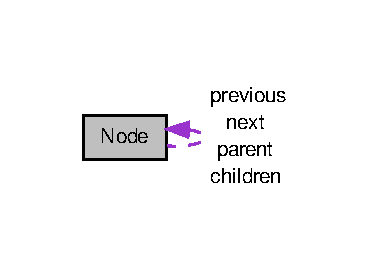
\includegraphics[width=178pt]{structNode__coll__graph}
\end{center}
\end{figure}
\subsection*{Data Fields}
\begin{DoxyCompactItemize}
\item 
enum \hyperlink{node_8h_a83ba1e84fa23f6619c3d29036b160919}{Node\-Tag} \hyperlink{structNode_aae55c9a8e76121d7f9c721c0239e6fb8}{tag}
\begin{DoxyCompactList}\small\item\em The tag of the \hyperlink{structNode}{Node}, specifying the type of the node. \end{DoxyCompactList}\item 
struct \hyperlink{structNode}{Node} $\ast$ \hyperlink{structNode_aa162dd1e0693188a22b1f13b9a2a0ef0}{next}
\begin{DoxyCompactList}\small\item\em Pointer to the next \hyperlink{structNode}{Node}. \end{DoxyCompactList}\item 
struct \hyperlink{structNode}{Node} $\ast$ \hyperlink{structNode_a9a9311efc5dc64017bf492a386b77b0d}{previous}
\begin{DoxyCompactList}\small\item\em Pointer to the previous \hyperlink{structNode}{Node}. \end{DoxyCompactList}\item 
struct \hyperlink{structNode}{Node} $\ast$ \hyperlink{structNode_a827ac726d02ddf6d00ba8a55cd296df2}{children}
\begin{DoxyCompactList}\small\item\em Pointer to the first child \hyperlink{structNode}{Node}. \end{DoxyCompactList}\item 
struct \hyperlink{structNode}{Node} $\ast$ \hyperlink{structNode_a7b739036012f282683e6452a0b1595af}{parent}
\begin{DoxyCompactList}\small\item\em Pointer to the previous \hyperlink{structNode}{Node}. \end{DoxyCompactList}\item 
double \hyperlink{structNode_ad7f9455e819b623c0e4a9480476eacfe}{ival}
\begin{DoxyCompactList}\small\item\em Value of the number represented by this \hyperlink{structNode}{Node}. \end{DoxyCompactList}\item 
char $\ast$ \hyperlink{structNode_a76c70ae7ac3d58ebe41da968fedb8093}{iname}
\begin{DoxyCompactList}\small\item\em The name of the identifier represented by this \hyperlink{structNode}{Node}. \end{DoxyCompactList}\item 
int \hyperlink{structNode_a28a2a20ee60bdfbd168e4f4bf20d8c82}{ignore}
\begin{DoxyCompactList}\small\item\em Property that will make parsers ignore the current assignment if set to 1. \end{DoxyCompactList}\end{DoxyCompactItemize}


\subsection{Detailed Description}
A two dimensional node/tree data. 

This data structure consists of nodes that specify their neighbours. Each node has a left neighbour, right neighbour, parent and children, resulting in a structure like this\-: \begin{DoxyVerb}node-1
  |-> node-1.1
  |-> node-1.2 
\end{DoxyVerb}
 Where node-\/1 has no neighbours, but two \hyperlink{structNode_a827ac726d02ddf6d00ba8a55cd296df2}{Node\-::children}\-: node-\/1.\-1 and node-\/1.\-2. node-\/1.\-1 is positioned \hyperlink{structNode_a9a9311efc5dc64017bf492a386b77b0d}{Node\-::previous} of node-\/1.\-2, whereas node-\/1.\-2 is the \hyperlink{structNode_aa162dd1e0693188a22b1f13b9a2a0ef0}{Node\-::next} node relative to node-\/1.\-1. Both node-\/1.\-1 and node-\/1.\-2 have node-\/1 as \hyperlink{structNode_a7b739036012f282683e6452a0b1595af}{Node\-::parent}.

Each node also has a \hyperlink{structNode_aae55c9a8e76121d7f9c721c0239e6fb8}{Node\-::tag}, defining the type of the node. Examples of tags are \hyperlink{node_8h_a83ba1e84fa23f6619c3d29036b160919ab61d4391af9740a542e317b9ce6a3d2e}{T\-P\-L\-U\-S} and \hyperlink{node_8h_a83ba1e84fa23f6619c3d29036b160919a2f6da8014bbb780265737f3edb98f928}{T\-M\-U\-L}, specifying a plus (+) or multiplication ($\ast$) operation respectively.

If the node specifies a number (i.\-e. the tag is \hyperlink{node_8h_a83ba1e84fa23f6619c3d29036b160919a71fff872f388505135681e9fad482e72}{T\-N\-U\-M}), \hyperlink{structNode_ad7f9455e819b623c0e4a9480476eacfe}{Node\-::ival} will hold the value of this number. Every number is interpreted as a double precision number, since Matlab does not really distinguishes between integers and floating point numbers either.

The \hyperlink{structNode_a76c70ae7ac3d58ebe41da968fedb8093}{Node\-::iname} property can be used in combination with the \hyperlink{node_8h_a83ba1e84fa23f6619c3d29036b160919afe64957b6fe1c660804c3d310000b5f0}{T\-V\-A\-R}, \hyperlink{node_8h_a83ba1e84fa23f6619c3d29036b160919a5b179cf7f0b8747fa3f686c8d7cdc2aa}{T\-A\-R\-R\-A\-Y\-I\-N\-D\-E\-X} or \hyperlink{node_8h_a83ba1e84fa23f6619c3d29036b160919aae1cac6fabc93853164889cdc0d77b1a}{T\-F\-O\-R} tags to specify the name of the identifier used.

The \hyperlink{structNode_a28a2a20ee60bdfbd168e4f4bf20d8c82}{Node\-::ignore} property can be used to ignore Matlab specific assignments that should not be translated to Fortran code.

\begin{DoxySeeAlso}{See Also}
\hyperlink{node_8h_a630e9a32f8dad634171441534eedd274}{copy\-Node}, \hyperlink{node_8h_a9404ea17c515d0d18c37bde7c31b5979}{remove\-Node}, \hyperlink{node_8h_a990974952aa48d789ee7dabf10070194}{create\-Operation}, \hyperlink{node_8h_aa603e9647cbbe4208a6de5546df7b9f7}{create\-Constant}, \hyperlink{node_8h_a25b6be3754d0bfe7f721c65986872f75}{create\-Variable}, \hyperlink{node_8h_ac59e12e2146890bd3656810716854c5f}{append\-Child}, \hyperlink{tree_8h_a4035da3929ae669ab801f4eff738bb6e}{print\-\_\-tree} 
\end{DoxySeeAlso}


\subsection{Field Documentation}
\hypertarget{structNode_a827ac726d02ddf6d00ba8a55cd296df2}{\index{Node@{Node}!children@{children}}
\index{children@{children}!Node@{Node}}
\subsubsection[{children}]{\setlength{\rightskip}{0pt plus 5cm}struct {\bf Node}$\ast$ children}}\label{structNode_a827ac726d02ddf6d00ba8a55cd296df2}


Pointer to the first child \hyperlink{structNode}{Node}. 

All other children can be accessed using the \hyperlink{structNode_aa162dd1e0693188a22b1f13b9a2a0ef0}{Node\-::next} properties of the children. Null when the \hyperlink{structNode}{Node} does not have children. \hypertarget{structNode_a28a2a20ee60bdfbd168e4f4bf20d8c82}{\index{Node@{Node}!ignore@{ignore}}
\index{ignore@{ignore}!Node@{Node}}
\subsubsection[{ignore}]{\setlength{\rightskip}{0pt plus 5cm}int ignore}}\label{structNode_a28a2a20ee60bdfbd168e4f4bf20d8c82}


Property that will make parsers ignore the current assignment if set to 1. 

\hypertarget{structNode_a76c70ae7ac3d58ebe41da968fedb8093}{\index{Node@{Node}!iname@{iname}}
\index{iname@{iname}!Node@{Node}}
\subsubsection[{iname}]{\setlength{\rightskip}{0pt plus 5cm}char$\ast$ iname}}\label{structNode_a76c70ae7ac3d58ebe41da968fedb8093}


The name of the identifier represented by this \hyperlink{structNode}{Node}. 

This property is only set when the tag of the \hyperlink{structNode}{Node} is either \hyperlink{node_8h_a83ba1e84fa23f6619c3d29036b160919afe64957b6fe1c660804c3d310000b5f0}{T\-V\-A\-R}, T\-A\-R\-R\-A\-Y\-I\-N\-D\-E\-X or \hyperlink{node_8h_a83ba1e84fa23f6619c3d29036b160919aae1cac6fabc93853164889cdc0d77b1a}{T\-F\-O\-R}. In the case of \hyperlink{node_8h_a83ba1e84fa23f6619c3d29036b160919afe64957b6fe1c660804c3d310000b5f0}{T\-V\-A\-R} and T\-A\-R\-R\-A\-Y\-I\-N\-D\-E\-X, this property specifies the name of the variable. When the tag is \hyperlink{node_8h_a83ba1e84fa23f6619c3d29036b160919aae1cac6fabc93853164889cdc0d77b1a}{T\-F\-O\-R}, this property specifies the name of the variable that is used by the for statement. \hypertarget{structNode_ad7f9455e819b623c0e4a9480476eacfe}{\index{Node@{Node}!ival@{ival}}
\index{ival@{ival}!Node@{Node}}
\subsubsection[{ival}]{\setlength{\rightskip}{0pt plus 5cm}double ival}}\label{structNode_ad7f9455e819b623c0e4a9480476eacfe}


Value of the number represented by this \hyperlink{structNode}{Node}. 

This property is only set when the tag of the \hyperlink{structNode}{Node} is \hyperlink{node_8h_a83ba1e84fa23f6619c3d29036b160919a71fff872f388505135681e9fad482e72}{T\-N\-U\-M}. \hypertarget{structNode_aa162dd1e0693188a22b1f13b9a2a0ef0}{\index{Node@{Node}!next@{next}}
\index{next@{next}!Node@{Node}}
\subsubsection[{next}]{\setlength{\rightskip}{0pt plus 5cm}struct {\bf Node}$\ast$ next}}\label{structNode_aa162dd1e0693188a22b1f13b9a2a0ef0}


Pointer to the next \hyperlink{structNode}{Node}. 

N\-U\-L\-L when the \hyperlink{structNode}{Node} does not have a next neighbour. \hypertarget{structNode_a7b739036012f282683e6452a0b1595af}{\index{Node@{Node}!parent@{parent}}
\index{parent@{parent}!Node@{Node}}
\subsubsection[{parent}]{\setlength{\rightskip}{0pt plus 5cm}struct {\bf Node}$\ast$ parent}}\label{structNode_a7b739036012f282683e6452a0b1595af}


Pointer to the previous \hyperlink{structNode}{Node}. 

N\-U\-L\-L when the \hyperlink{structNode}{Node} is the topmost \hyperlink{structNode}{Node}. \hypertarget{structNode_a9a9311efc5dc64017bf492a386b77b0d}{\index{Node@{Node}!previous@{previous}}
\index{previous@{previous}!Node@{Node}}
\subsubsection[{previous}]{\setlength{\rightskip}{0pt plus 5cm}struct {\bf Node}$\ast$ previous}}\label{structNode_a9a9311efc5dc64017bf492a386b77b0d}


Pointer to the previous \hyperlink{structNode}{Node}. 

N\-U\-L\-L when the \hyperlink{structNode}{Node} does not have a previous neighbour. \hypertarget{structNode_aae55c9a8e76121d7f9c721c0239e6fb8}{\index{Node@{Node}!tag@{tag}}
\index{tag@{tag}!Node@{Node}}
\subsubsection[{tag}]{\setlength{\rightskip}{0pt plus 5cm}enum {\bf Node\-Tag} tag}}\label{structNode_aae55c9a8e76121d7f9c721c0239e6fb8}


The tag of the \hyperlink{structNode}{Node}, specifying the type of the node. 



The documentation for this struct was generated from the following file\-:\begin{DoxyCompactItemize}
\item 
\hyperlink{node_8h}{node.\-h}\end{DoxyCompactItemize}

\hypertarget{structVariable}{\section{Variable Struct Reference}
\label{structVariable}\index{Variable@{Variable}}
}


Datatype of a variable.  




{\ttfamily \#include $<$tree.\-h$>$}



Collaboration diagram for Variable\-:\nopagebreak
\begin{figure}[H]
\begin{center}
\leavevmode
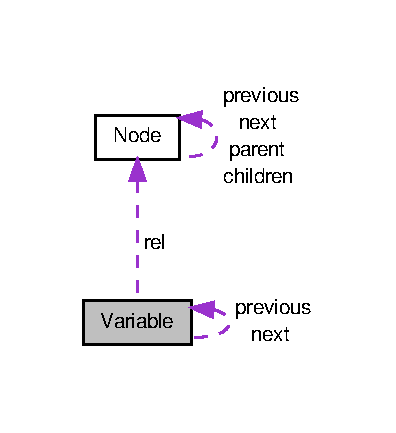
\includegraphics[width=190pt]{structVariable__coll__graph}
\end{center}
\end{figure}
\subsection*{Data Fields}
\begin{DoxyCompactItemize}
\item 
enum \hyperlink{tree_8h_ac62972ff1b21a037e56530cde67309ab}{Variable\-Type} \hyperlink{structVariable_a6d3af05ac5e896c45aeb8834fcbf84f4}{type}
\begin{DoxyCompactList}\small\item\em Type of the variable. \end{DoxyCompactList}\item 
struct \hyperlink{structVariable}{Variable} $\ast$ \hyperlink{structVariable_ac6387180163bef05cf8ea37a4fbd0682}{next}
\begin{DoxyCompactList}\small\item\em Pointer to the next variable in the linked list. \end{DoxyCompactList}\item 
struct \hyperlink{structVariable}{Variable} $\ast$ \hyperlink{structVariable_ad27df2f2e773678c5804cc233343aed1}{previous}
\begin{DoxyCompactList}\small\item\em Pointer to the previous variable in the linked list. \end{DoxyCompactList}\item 
char $\ast$ \hyperlink{structVariable_a76c70ae7ac3d58ebe41da968fedb8093}{iname}
\begin{DoxyCompactList}\small\item\em Name/identifier of the variable. \end{DoxyCompactList}\item 
struct \hyperlink{structNode}{Node} $\ast$ \hyperlink{structVariable_adf9b74cb9b4f3a80e8af89e50bd11975}{rel}
\begin{DoxyCompactList}\small\item\em The relation of the variable to the independent variable of the O\-D\-E system. \end{DoxyCompactList}\item 
int \hyperlink{structVariable_a627f44b64b5d8d3ae8cb6a675f164405}{zero}
\begin{DoxyCompactList}\small\item\em 1 when this variable is always zero, 0 otherwise. \end{DoxyCompactList}\end{DoxyCompactItemize}


\subsection{Detailed Description}
Datatype of a variable. 

This datatype can hold information about the type and name of the variable. It is also a linked list. 

\subsection{Field Documentation}
\hypertarget{structVariable_a76c70ae7ac3d58ebe41da968fedb8093}{\index{Variable@{Variable}!iname@{iname}}
\index{iname@{iname}!Variable@{Variable}}
\subsubsection[{iname}]{\setlength{\rightskip}{0pt plus 5cm}char$\ast$ iname}}\label{structVariable_a76c70ae7ac3d58ebe41da968fedb8093}


Name/identifier of the variable. 

\hypertarget{structVariable_ac6387180163bef05cf8ea37a4fbd0682}{\index{Variable@{Variable}!next@{next}}
\index{next@{next}!Variable@{Variable}}
\subsubsection[{next}]{\setlength{\rightskip}{0pt plus 5cm}struct {\bf Variable}$\ast$ next}}\label{structVariable_ac6387180163bef05cf8ea37a4fbd0682}


Pointer to the next variable in the linked list. 

\hypertarget{structVariable_ad27df2f2e773678c5804cc233343aed1}{\index{Variable@{Variable}!previous@{previous}}
\index{previous@{previous}!Variable@{Variable}}
\subsubsection[{previous}]{\setlength{\rightskip}{0pt plus 5cm}struct {\bf Variable}$\ast$ previous}}\label{structVariable_ad27df2f2e773678c5804cc233343aed1}


Pointer to the previous variable in the linked list. 

\hypertarget{structVariable_adf9b74cb9b4f3a80e8af89e50bd11975}{\index{Variable@{Variable}!rel@{rel}}
\index{rel@{rel}!Variable@{Variable}}
\subsubsection[{rel}]{\setlength{\rightskip}{0pt plus 5cm}struct {\bf Node}$\ast$ rel}}\label{structVariable_adf9b74cb9b4f3a80e8af89e50bd11975}


The relation of the variable to the independent variable of the O\-D\-E system. 

\hypertarget{structVariable_a6d3af05ac5e896c45aeb8834fcbf84f4}{\index{Variable@{Variable}!type@{type}}
\index{type@{type}!Variable@{Variable}}
\subsubsection[{type}]{\setlength{\rightskip}{0pt plus 5cm}enum {\bf Variable\-Type} type}}\label{structVariable_a6d3af05ac5e896c45aeb8834fcbf84f4}


Type of the variable. 

\hypertarget{structVariable_a627f44b64b5d8d3ae8cb6a675f164405}{\index{Variable@{Variable}!zero@{zero}}
\index{zero@{zero}!Variable@{Variable}}
\subsubsection[{zero}]{\setlength{\rightskip}{0pt plus 5cm}int zero}}\label{structVariable_a627f44b64b5d8d3ae8cb6a675f164405}


1 when this variable is always zero, 0 otherwise. 



The documentation for this struct was generated from the following file\-:\begin{DoxyCompactItemize}
\item 
\hyperlink{tree_8h}{tree.\-h}\end{DoxyCompactItemize}

\chapter{File Documentation}
\hypertarget{fortran_8c}{\section{fortran.\-c File Reference}
\label{fortran_8c}\index{fortran.\-c@{fortran.\-c}}
}
{\ttfamily \#include $<$stdio.\-h$>$}\\*
{\ttfamily \#include $<$stdlib.\-h$>$}\\*
{\ttfamily \#include $<$string.\-h$>$}\\*
{\ttfamily \#include \char`\"{}fortran.\-h\char`\"{}}\\*
{\ttfamily \#include \char`\"{}jacobian.\-h\char`\"{}}\\*
{\ttfamily \#include \char`\"{}tree.\-h\char`\"{}}\\*
{\ttfamily \#include \char`\"{}node.\-h\char`\"{}}\\*
Include dependency graph for fortran.\-c\-:\nopagebreak
\begin{figure}[H]
\begin{center}
\leavevmode
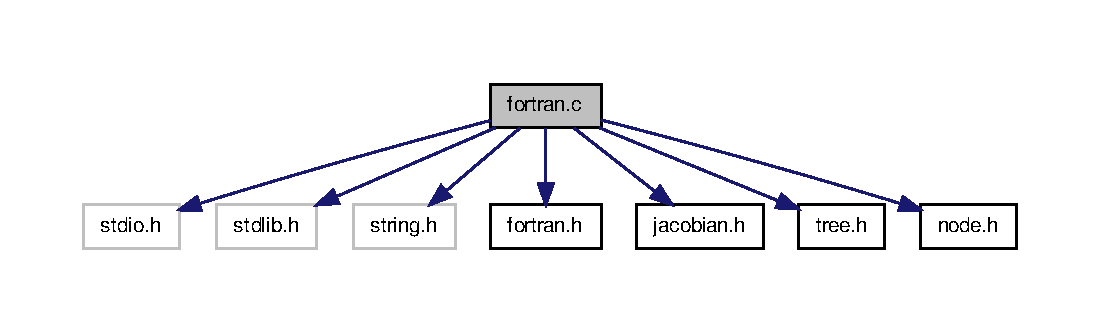
\includegraphics[width=350pt]{fortran_8c__incl}
\end{center}
\end{figure}
\subsection*{Macros}
\begin{DoxyCompactItemize}
\item 
\#define \hyperlink{fortran_8c_a369266c24eacffb87046522897a570d5}{\-\_\-\-G\-N\-U\-\_\-\-S\-O\-U\-R\-C\-E}
\end{DoxyCompactItemize}
\subsection*{Functions}
\begin{DoxyCompactItemize}
\item 
void \hyperlink{fortran_8c_a2222da9d792b8540ffba7e25fbf4e4a4}{function\-To\-Fortran} (struct \hyperlink{structNode}{Node} $\ast$t)
\begin{DoxyCompactList}\small\item\em Translate a O\-D\-E function to Fortran. \end{DoxyCompactList}\item 
void \hyperlink{fortran_8c_a6d57af6f238f091e9c62b9ed81f194a3}{print\-Fortran\-Function} (struct \hyperlink{structNode}{Node} $\ast$t, int jac)
\begin{DoxyCompactList}\small\item\em Translate a O\-D\-E or Jacobian function to Fortran. \end{DoxyCompactList}\item 
char $\ast$ \hyperlink{fortran_8c_a712ba008f0345618c5b1b87358a0206e}{to\-Fortran} (struct \hyperlink{structNode}{Node} $\ast$t)
\begin{DoxyCompactList}\small\item\em Recursively translate a Nodes to Fortran. \end{DoxyCompactList}\item 
char $\ast$ \hyperlink{fortran_8c_a02a98fd967252e6d807915856d09c77f}{F\-\_\-plus} (char $\ast$s1, char $\ast$s2)
\begin{DoxyCompactList}\small\item\em Generate Fortran code representing a plus (+) operation. \end{DoxyCompactList}\item 
char $\ast$ \hyperlink{fortran_8c_adc9b028cf89661eeb91182ab007da632}{F\-\_\-minus} (char $\ast$s1, char $\ast$s2)
\begin{DoxyCompactList}\small\item\em Generate Fortran code representing a minus (-\/) operation. \end{DoxyCompactList}\item 
char $\ast$ \hyperlink{fortran_8c_a0ca25a9453e2eeb469f1120368dd481f}{F\-\_\-negative} (char $\ast$s1)
\begin{DoxyCompactList}\small\item\em Generate Fortran code representing a negative sign (-\/) operation. \end{DoxyCompactList}\item 
char $\ast$ \hyperlink{fortran_8c_a1d67a9cba2734d4accc1f041aeab29dc}{F\-\_\-mul} (char $\ast$s1, char $\ast$s2)
\begin{DoxyCompactList}\small\item\em Generate Fortran code representing a multiplication ($\ast$) operation. \end{DoxyCompactList}\item 
char $\ast$ \hyperlink{fortran_8c_a0a05ea2fc6b0ca74871f60f1580fade0}{F\-\_\-div} (char $\ast$s1, char $\ast$s2)
\begin{DoxyCompactList}\small\item\em Generate Fortran code representing a division (/) operation. \end{DoxyCompactList}\item 
char $\ast$ \hyperlink{fortran_8c_ab1deef2cd69a27b35060de99428d6002}{F\-\_\-pow} (char $\ast$s1, char $\ast$s2)
\begin{DoxyCompactList}\small\item\em Generate Fortran code representing a power ($^\wedge$) operation. \end{DoxyCompactList}\item 
char $\ast$ \hyperlink{fortran_8c_ad039b3cb32f255dbab046b141de3b710}{F\-\_\-not} (char $\ast$s1)
\begin{DoxyCompactList}\small\item\em Generate Fortran code representing a N\-O\-T ($\sim$, !) operation. \end{DoxyCompactList}\item 
char $\ast$ \hyperlink{fortran_8c_a87a3641482ea51fff74931c9248ce245}{F\-\_\-or} (char $\ast$s1, char $\ast$s2)
\begin{DoxyCompactList}\small\item\em Generate Fortran code representing an O\-R ($|$$|$) operation. \end{DoxyCompactList}\item 
char $\ast$ \hyperlink{fortran_8c_a0cd8a485e5575fe231bd15bb724c904f}{F\-\_\-and} (char $\ast$s1, char $\ast$s2)
\begin{DoxyCompactList}\small\item\em Generate Fortran code representing an A\-N\-D (\&\&) operation. \end{DoxyCompactList}\item 
char $\ast$ \hyperlink{fortran_8c_a46ec6c338eb4bc765f191f1c4c3a4b53}{F\-\_\-eq\-\_\-op} (char $\ast$s1, char $\ast$s2)
\begin{DoxyCompactList}\small\item\em Generate Fortran code representing a E\-Q\-U\-A\-L (==) operation. \end{DoxyCompactList}\item 
char $\ast$ \hyperlink{fortran_8c_afaf4bf6f26417c1e1abb46f4a67b3d90}{F\-\_\-ne\-\_\-op} (char $\ast$s1, char $\ast$s2)
\begin{DoxyCompactList}\small\item\em Generate Fortran code representing a N\-O\-T E\-Q\-U\-A\-L ($\sim$=, !=) operation. \end{DoxyCompactList}\item 
char $\ast$ \hyperlink{fortran_8c_a97a8bc56d7ed7fee3bff400d1fd58ea3}{F\-\_\-gt\-\_\-op} (char $\ast$s1, char $\ast$s2)
\begin{DoxyCompactList}\small\item\em Generate Fortran code representing a G\-R\-E\-A\-T\-E\-R T\-H\-A\-N ($>$) operation. \end{DoxyCompactList}\item 
char $\ast$ \hyperlink{fortran_8c_ae69df0da134bdabf8e931d0f18f9a9de}{F\-\_\-ge\-\_\-op} (char $\ast$s1, char $\ast$s2)
\begin{DoxyCompactList}\small\item\em Generate Fortran code representing a G\-R\-E\-A\-T\-E\-R O\-R E\-Q\-U\-A\-L ($>$=) operation. \end{DoxyCompactList}\item 
char $\ast$ \hyperlink{fortran_8c_a168e6ceafab728511a2832d50e48942a}{F\-\_\-lt\-\_\-op} (char $\ast$s1, char $\ast$s2)
\begin{DoxyCompactList}\small\item\em Generate Fortran code representing a L\-E\-S\-S\-E\-R T\-H\-A\-N ($<$) operation. \end{DoxyCompactList}\item 
char $\ast$ \hyperlink{fortran_8c_a9b9a6759bf60f4ee7f53eb2af65acf05}{F\-\_\-le\-\_\-op} (char $\ast$s1, char $\ast$s2)
\begin{DoxyCompactList}\small\item\em Generate Fortran code representing a L\-E\-S\-S\-E\-R O\-R E\-Q\-U\-A\-L ($<$=) operation. \end{DoxyCompactList}\item 
char $\ast$ \hyperlink{fortran_8c_a3a9a87b9a8262532d796ae4904caac49}{F\-\_\-assign} (char $\ast$s1, char $\ast$s2)
\begin{DoxyCompactList}\small\item\em Generate Fortran code representing an assign (=) statement. \end{DoxyCompactList}\item 
char $\ast$ \hyperlink{fortran_8c_abafedd063906b6369ffadd0d9ec36f9e}{F\-\_\-for} (char $\ast$s1, char $\ast$s2, char $\ast$s3)
\begin{DoxyCompactList}\small\item\em Generate Fortran code representing a for statement. \end{DoxyCompactList}\item 
char $\ast$ \hyperlink{fortran_8c_aa6f504e52bf6b28f12fcb6f052642d04}{F\-\_\-range} (char $\ast$s1, char $\ast$s2, char $\ast$s3)
\begin{DoxyCompactList}\small\item\em Generate Fortran code representing a range (\-:) operation. \end{DoxyCompactList}\item 
char $\ast$ \hyperlink{fortran_8c_a6fc4168f0113431f451b2fbc8a23cd39}{F\-\_\-while} (char $\ast$s1, char $\ast$s2)
\begin{DoxyCompactList}\small\item\em Generate Fortran code representing a while statement. \end{DoxyCompactList}\item 
char $\ast$ \hyperlink{fortran_8c_ad35c68cadde4047a250fc7f3722cd4ba}{F\-\_\-if} (char $\ast$s1, char $\ast$s2)
\item 
char $\ast$ \hyperlink{fortran_8c_a9d12d2fadabc5cb43dcfd3da0a379a27}{F\-\_\-ifelse} (char $\ast$s1, char $\ast$s2, char $\ast$s3)
\item 
char $\ast$ \hyperlink{fortran_8c_aa40f8274e7e8d72e7bf45b8ba657b487}{F\-\_\-ifelseif} (char $\ast$s1, char $\ast$s2, char $\ast$s3)
\item 
char $\ast$ \hyperlink{fortran_8c_ae4f68d273f9c36127d05c8ce3036599e}{F\-\_\-elseif} (char $\ast$s1, char $\ast$s2)
\item 
char $\ast$ \hyperlink{fortran_8c_a3c18e2e40028988c33e5513716e00395}{F\-\_\-ifelseifelse} (char $\ast$s1, char $\ast$s2, char $\ast$s3, char $\ast$s4)
\item 
char $\ast$ \hyperlink{fortran_8c_abcfc636d10b338ba9603adc5080f8268}{F\-\_\-arrayindex} (char $\ast$s1, char $\ast$s2)
\begin{DoxyCompactList}\small\item\em Generate Fortran code representing an array indexing (a\mbox{[}b\mbox{]}) operation. \end{DoxyCompactList}\item 
char $\ast$ \hyperlink{fortran_8c_ae7130ea548b657055bbd08670caa7361}{F\-\_\-indexrange} (char $\ast$s1, char $\ast$s2)
\begin{DoxyCompactList}\small\item\em Generate Fortran code representing a range (\-:) operation. \end{DoxyCompactList}\item 
char $\ast$ \hyperlink{fortran_8c_ab230e89691dc4f8dff8d85472c20fd8a}{F\-\_\-zeros} (char $\ast$s1, char $\ast$s2, int allocate)
\item 
char $\ast$ \hyperlink{fortran_8c_a4193d629b89c1551beb365d1c0a4bc13}{F\-\_\-combine} (char $\ast$s1, char $\ast$s2)
\begin{DoxyCompactList}\small\item\em Generate Fortran code representing the subsequent execution of two statements. \end{DoxyCompactList}\item 
char $\ast$ \hyperlink{fortran_8c_a9a1c3a7f211f7d42c6dedcdaed68067e}{line} (int label, char $\ast$content)
\begin{DoxyCompactList}\small\item\em Fit a string into the Fortran fixed format. \end{DoxyCompactList}\end{DoxyCompactItemize}


\subsection{Macro Definition Documentation}
\hypertarget{fortran_8c_a369266c24eacffb87046522897a570d5}{\index{fortran.\-c@{fortran.\-c}!\-\_\-\-G\-N\-U\-\_\-\-S\-O\-U\-R\-C\-E@{\-\_\-\-G\-N\-U\-\_\-\-S\-O\-U\-R\-C\-E}}
\index{\-\_\-\-G\-N\-U\-\_\-\-S\-O\-U\-R\-C\-E@{\-\_\-\-G\-N\-U\-\_\-\-S\-O\-U\-R\-C\-E}!fortran.c@{fortran.\-c}}
\subsubsection[{\-\_\-\-G\-N\-U\-\_\-\-S\-O\-U\-R\-C\-E}]{\setlength{\rightskip}{0pt plus 5cm}\#define \-\_\-\-G\-N\-U\-\_\-\-S\-O\-U\-R\-C\-E}}\label{fortran_8c_a369266c24eacffb87046522897a570d5}


\subsection{Function Documentation}
\hypertarget{fortran_8c_a0cd8a485e5575fe231bd15bb724c904f}{\index{fortran.\-c@{fortran.\-c}!F\-\_\-and@{F\-\_\-and}}
\index{F\-\_\-and@{F\-\_\-and}!fortran.c@{fortran.\-c}}
\subsubsection[{F\-\_\-and}]{\setlength{\rightskip}{0pt plus 5cm}char$\ast$ F\-\_\-and (
\begin{DoxyParamCaption}
\item[{char $\ast$}]{s1, }
\item[{char $\ast$}]{s2}
\end{DoxyParamCaption}
)}}\label{fortran_8c_a0cd8a485e5575fe231bd15bb724c904f}


Generate Fortran code representing an A\-N\-D (\&\&) operation. 

Generate Fortran code that applies an A\-N\-D (\&\&) operation on the code segments represented by {\itshape s1} and {\itshape s2} (s1 \&\& s2). 
\begin{DoxyParams}{Parameters}
{\em s1} & First code segment. \\
\hline
{\em s2} & Second code segment. \\
\hline
\end{DoxyParams}
\begin{DoxyReturn}{Returns}
The Fortran code. 
\end{DoxyReturn}
\hypertarget{fortran_8c_abcfc636d10b338ba9603adc5080f8268}{\index{fortran.\-c@{fortran.\-c}!F\-\_\-arrayindex@{F\-\_\-arrayindex}}
\index{F\-\_\-arrayindex@{F\-\_\-arrayindex}!fortran.c@{fortran.\-c}}
\subsubsection[{F\-\_\-arrayindex}]{\setlength{\rightskip}{0pt plus 5cm}char$\ast$ F\-\_\-arrayindex (
\begin{DoxyParamCaption}
\item[{char $\ast$}]{s1, }
\item[{char $\ast$}]{s2}
\end{DoxyParamCaption}
)}}\label{fortran_8c_abcfc636d10b338ba9603adc5080f8268}


Generate Fortran code representing an array indexing (a\mbox{[}b\mbox{]}) operation. 

Generate Fortran code that applies an array indexing (a\mbox{[}b\mbox{]}) operation on the code segments represented by {\itshape s1} and {\itshape s2} (s1\mbox{[}s2\mbox{]}). 
\begin{DoxyParams}{Parameters}
{\em s1} & First code segment. \\
\hline
{\em s2} & Second code segment. \\
\hline
\end{DoxyParams}
\begin{DoxyReturn}{Returns}
The Fortran code. 
\end{DoxyReturn}
\hypertarget{fortran_8c_a3a9a87b9a8262532d796ae4904caac49}{\index{fortran.\-c@{fortran.\-c}!F\-\_\-assign@{F\-\_\-assign}}
\index{F\-\_\-assign@{F\-\_\-assign}!fortran.c@{fortran.\-c}}
\subsubsection[{F\-\_\-assign}]{\setlength{\rightskip}{0pt plus 5cm}char$\ast$ F\-\_\-assign (
\begin{DoxyParamCaption}
\item[{char $\ast$}]{s1, }
\item[{char $\ast$}]{s2}
\end{DoxyParamCaption}
)}}\label{fortran_8c_a3a9a87b9a8262532d796ae4904caac49}


Generate Fortran code representing an assign (=) statement. 

Generate Fortran code that applies an assign (=) statement on the code segments represented by {\itshape s1} and {\itshape s2} (s1 = s2). 
\begin{DoxyParams}{Parameters}
{\em s1} & First code segment. \\
\hline
{\em s2} & Second code segment. \\
\hline
\end{DoxyParams}
\begin{DoxyReturn}{Returns}
The Fortran code. 
\end{DoxyReturn}
\hypertarget{fortran_8c_a4193d629b89c1551beb365d1c0a4bc13}{\index{fortran.\-c@{fortran.\-c}!F\-\_\-combine@{F\-\_\-combine}}
\index{F\-\_\-combine@{F\-\_\-combine}!fortran.c@{fortran.\-c}}
\subsubsection[{F\-\_\-combine}]{\setlength{\rightskip}{0pt plus 5cm}char$\ast$ F\-\_\-combine (
\begin{DoxyParamCaption}
\item[{char $\ast$}]{s1, }
\item[{char $\ast$}]{s2}
\end{DoxyParamCaption}
)}}\label{fortran_8c_a4193d629b89c1551beb365d1c0a4bc13}


Generate Fortran code representing the subsequent execution of two statements. 

Generate Fortran code that subsequently executes {\itshape s1} and {\itshape s2} (s1;s2). 
\begin{DoxyParams}{Parameters}
{\em s1} & First code segment. \\
\hline
{\em s2} & Second code segment. \\
\hline
\end{DoxyParams}
\begin{DoxyReturn}{Returns}
The Fortran code. 
\end{DoxyReturn}
\hypertarget{fortran_8c_a0a05ea2fc6b0ca74871f60f1580fade0}{\index{fortran.\-c@{fortran.\-c}!F\-\_\-div@{F\-\_\-div}}
\index{F\-\_\-div@{F\-\_\-div}!fortran.c@{fortran.\-c}}
\subsubsection[{F\-\_\-div}]{\setlength{\rightskip}{0pt plus 5cm}char$\ast$ F\-\_\-div (
\begin{DoxyParamCaption}
\item[{char $\ast$}]{s1, }
\item[{char $\ast$}]{s2}
\end{DoxyParamCaption}
)}}\label{fortran_8c_a0a05ea2fc6b0ca74871f60f1580fade0}


Generate Fortran code representing a division (/) operation. 

Generate Fortran code that applies a division (/) operation on the code segments represented by {\itshape s1} and {\itshape s2} (s1 / s2). 
\begin{DoxyParams}{Parameters}
{\em s1} & First code segment. \\
\hline
{\em s2} & Second code segment. \\
\hline
\end{DoxyParams}
\begin{DoxyReturn}{Returns}
The Fortran code. 
\end{DoxyReturn}
\hypertarget{fortran_8c_ae4f68d273f9c36127d05c8ce3036599e}{\index{fortran.\-c@{fortran.\-c}!F\-\_\-elseif@{F\-\_\-elseif}}
\index{F\-\_\-elseif@{F\-\_\-elseif}!fortran.c@{fortran.\-c}}
\subsubsection[{F\-\_\-elseif}]{\setlength{\rightskip}{0pt plus 5cm}char$\ast$ F\-\_\-elseif (
\begin{DoxyParamCaption}
\item[{char $\ast$}]{s1, }
\item[{char $\ast$}]{s2}
\end{DoxyParamCaption}
)}}\label{fortran_8c_ae4f68d273f9c36127d05c8ce3036599e}
\hypertarget{fortran_8c_a46ec6c338eb4bc765f191f1c4c3a4b53}{\index{fortran.\-c@{fortran.\-c}!F\-\_\-eq\-\_\-op@{F\-\_\-eq\-\_\-op}}
\index{F\-\_\-eq\-\_\-op@{F\-\_\-eq\-\_\-op}!fortran.c@{fortran.\-c}}
\subsubsection[{F\-\_\-eq\-\_\-op}]{\setlength{\rightskip}{0pt plus 5cm}char$\ast$ F\-\_\-eq\-\_\-op (
\begin{DoxyParamCaption}
\item[{char $\ast$}]{s1, }
\item[{char $\ast$}]{s2}
\end{DoxyParamCaption}
)}}\label{fortran_8c_a46ec6c338eb4bc765f191f1c4c3a4b53}


Generate Fortran code representing a E\-Q\-U\-A\-L (==) operation. 

Generate Fortran code that applies a E\-Q\-U\-A\-L (==) operation on the code segments represented by {\itshape s1} and {\itshape s2} (s1 == s2). 
\begin{DoxyParams}{Parameters}
{\em s1} & First code segment. \\
\hline
{\em s2} & Second code segment. \\
\hline
\end{DoxyParams}
\begin{DoxyReturn}{Returns}
The Fortran code. 
\end{DoxyReturn}
\hypertarget{fortran_8c_abafedd063906b6369ffadd0d9ec36f9e}{\index{fortran.\-c@{fortran.\-c}!F\-\_\-for@{F\-\_\-for}}
\index{F\-\_\-for@{F\-\_\-for}!fortran.c@{fortran.\-c}}
\subsubsection[{F\-\_\-for}]{\setlength{\rightskip}{0pt plus 5cm}char$\ast$ F\-\_\-for (
\begin{DoxyParamCaption}
\item[{char $\ast$}]{s1, }
\item[{char $\ast$}]{s2, }
\item[{char $\ast$}]{s3}
\end{DoxyParamCaption}
)}}\label{fortran_8c_abafedd063906b6369ffadd0d9ec36f9e}


Generate Fortran code representing a for statement. 

Generate Fortran code that applies a for statement on the code segments represented by {\itshape s1}, {\itshape s2} and {\itshape s3} (do {\itshape label} s1 = s2; s3; {\itshape label} continue). 
\begin{DoxyParams}{Parameters}
{\em s1} & First code segment. \\
\hline
{\em s2} & Second code segment. \\
\hline
{\em s3} & Third code segment. \\
\hline
\end{DoxyParams}
\begin{DoxyReturn}{Returns}
The Fortran code. 
\end{DoxyReturn}
\hypertarget{fortran_8c_ae69df0da134bdabf8e931d0f18f9a9de}{\index{fortran.\-c@{fortran.\-c}!F\-\_\-ge\-\_\-op@{F\-\_\-ge\-\_\-op}}
\index{F\-\_\-ge\-\_\-op@{F\-\_\-ge\-\_\-op}!fortran.c@{fortran.\-c}}
\subsubsection[{F\-\_\-ge\-\_\-op}]{\setlength{\rightskip}{0pt plus 5cm}char$\ast$ F\-\_\-ge\-\_\-op (
\begin{DoxyParamCaption}
\item[{char $\ast$}]{s1, }
\item[{char $\ast$}]{s2}
\end{DoxyParamCaption}
)}}\label{fortran_8c_ae69df0da134bdabf8e931d0f18f9a9de}


Generate Fortran code representing a G\-R\-E\-A\-T\-E\-R O\-R E\-Q\-U\-A\-L ($>$=) operation. 

Generate Fortran code that applies a G\-R\-E\-A\-T\-E\-R O\-R E\-Q\-U\-A\-L ($>$=) operation on the code segments represented by {\itshape s1} and {\itshape s2} (s1 $>$= s2). 
\begin{DoxyParams}{Parameters}
{\em s1} & First code segment. \\
\hline
{\em s2} & Second code segment. \\
\hline
\end{DoxyParams}
\begin{DoxyReturn}{Returns}
The Fortran code. 
\end{DoxyReturn}
\hypertarget{fortran_8c_a97a8bc56d7ed7fee3bff400d1fd58ea3}{\index{fortran.\-c@{fortran.\-c}!F\-\_\-gt\-\_\-op@{F\-\_\-gt\-\_\-op}}
\index{F\-\_\-gt\-\_\-op@{F\-\_\-gt\-\_\-op}!fortran.c@{fortran.\-c}}
\subsubsection[{F\-\_\-gt\-\_\-op}]{\setlength{\rightskip}{0pt plus 5cm}char$\ast$ F\-\_\-gt\-\_\-op (
\begin{DoxyParamCaption}
\item[{char $\ast$}]{s1, }
\item[{char $\ast$}]{s2}
\end{DoxyParamCaption}
)}}\label{fortran_8c_a97a8bc56d7ed7fee3bff400d1fd58ea3}


Generate Fortran code representing a G\-R\-E\-A\-T\-E\-R T\-H\-A\-N ($>$) operation. 

Generate Fortran code that applies a G\-R\-E\-A\-T\-E\-R T\-H\-A\-N ($>$) operation on the code segments represented by {\itshape s1} and {\itshape s2} (s1 $>$ s2). 
\begin{DoxyParams}{Parameters}
{\em s1} & First code segment. \\
\hline
{\em s2} & Second code segment. \\
\hline
\end{DoxyParams}
\begin{DoxyReturn}{Returns}
The Fortran code. 
\end{DoxyReturn}
\hypertarget{fortran_8c_ad35c68cadde4047a250fc7f3722cd4ba}{\index{fortran.\-c@{fortran.\-c}!F\-\_\-if@{F\-\_\-if}}
\index{F\-\_\-if@{F\-\_\-if}!fortran.c@{fortran.\-c}}
\subsubsection[{F\-\_\-if}]{\setlength{\rightskip}{0pt plus 5cm}char$\ast$ F\-\_\-if (
\begin{DoxyParamCaption}
\item[{char $\ast$}]{s1, }
\item[{char $\ast$}]{s2}
\end{DoxyParamCaption}
)}}\label{fortran_8c_ad35c68cadde4047a250fc7f3722cd4ba}
\hypertarget{fortran_8c_a9d12d2fadabc5cb43dcfd3da0a379a27}{\index{fortran.\-c@{fortran.\-c}!F\-\_\-ifelse@{F\-\_\-ifelse}}
\index{F\-\_\-ifelse@{F\-\_\-ifelse}!fortran.c@{fortran.\-c}}
\subsubsection[{F\-\_\-ifelse}]{\setlength{\rightskip}{0pt plus 5cm}char$\ast$ F\-\_\-ifelse (
\begin{DoxyParamCaption}
\item[{char $\ast$}]{s1, }
\item[{char $\ast$}]{s2, }
\item[{char $\ast$}]{s3}
\end{DoxyParamCaption}
)}}\label{fortran_8c_a9d12d2fadabc5cb43dcfd3da0a379a27}
\hypertarget{fortran_8c_aa40f8274e7e8d72e7bf45b8ba657b487}{\index{fortran.\-c@{fortran.\-c}!F\-\_\-ifelseif@{F\-\_\-ifelseif}}
\index{F\-\_\-ifelseif@{F\-\_\-ifelseif}!fortran.c@{fortran.\-c}}
\subsubsection[{F\-\_\-ifelseif}]{\setlength{\rightskip}{0pt plus 5cm}char$\ast$ F\-\_\-ifelseif (
\begin{DoxyParamCaption}
\item[{char $\ast$}]{s1, }
\item[{char $\ast$}]{s2, }
\item[{char $\ast$}]{s3}
\end{DoxyParamCaption}
)}}\label{fortran_8c_aa40f8274e7e8d72e7bf45b8ba657b487}
\hypertarget{fortran_8c_a3c18e2e40028988c33e5513716e00395}{\index{fortran.\-c@{fortran.\-c}!F\-\_\-ifelseifelse@{F\-\_\-ifelseifelse}}
\index{F\-\_\-ifelseifelse@{F\-\_\-ifelseifelse}!fortran.c@{fortran.\-c}}
\subsubsection[{F\-\_\-ifelseifelse}]{\setlength{\rightskip}{0pt plus 5cm}char$\ast$ F\-\_\-ifelseifelse (
\begin{DoxyParamCaption}
\item[{char $\ast$}]{s1, }
\item[{char $\ast$}]{s2, }
\item[{char $\ast$}]{s3, }
\item[{char $\ast$}]{s4}
\end{DoxyParamCaption}
)}}\label{fortran_8c_a3c18e2e40028988c33e5513716e00395}
\hypertarget{fortran_8c_ae7130ea548b657055bbd08670caa7361}{\index{fortran.\-c@{fortran.\-c}!F\-\_\-indexrange@{F\-\_\-indexrange}}
\index{F\-\_\-indexrange@{F\-\_\-indexrange}!fortran.c@{fortran.\-c}}
\subsubsection[{F\-\_\-indexrange}]{\setlength{\rightskip}{0pt plus 5cm}char$\ast$ F\-\_\-indexrange (
\begin{DoxyParamCaption}
\item[{char $\ast$}]{s1, }
\item[{char $\ast$}]{s2}
\end{DoxyParamCaption}
)}}\label{fortran_8c_ae7130ea548b657055bbd08670caa7361}


Generate Fortran code representing a range (\-:) operation. 

Generate Fortran code that applies a range (\-:) operation on the code segments represented by {\itshape s1} and {\itshape s2} preparing it for use in an array indexing expression (s1\-:s2). 
\begin{DoxyParams}{Parameters}
{\em s1} & First code segment. \\
\hline
{\em s2} & Second code segment. \\
\hline
\end{DoxyParams}
\begin{DoxyReturn}{Returns}
The Fortran code. 
\end{DoxyReturn}
\hypertarget{fortran_8c_a9b9a6759bf60f4ee7f53eb2af65acf05}{\index{fortran.\-c@{fortran.\-c}!F\-\_\-le\-\_\-op@{F\-\_\-le\-\_\-op}}
\index{F\-\_\-le\-\_\-op@{F\-\_\-le\-\_\-op}!fortran.c@{fortran.\-c}}
\subsubsection[{F\-\_\-le\-\_\-op}]{\setlength{\rightskip}{0pt plus 5cm}char$\ast$ F\-\_\-le\-\_\-op (
\begin{DoxyParamCaption}
\item[{char $\ast$}]{s1, }
\item[{char $\ast$}]{s2}
\end{DoxyParamCaption}
)}}\label{fortran_8c_a9b9a6759bf60f4ee7f53eb2af65acf05}


Generate Fortran code representing a L\-E\-S\-S\-E\-R O\-R E\-Q\-U\-A\-L ($<$=) operation. 

Generate Fortran code that applies a L\-E\-S\-S\-E\-R O\-R E\-Q\-U\-A\-L ($<$=) operation on the code segments represented by {\itshape s1} and {\itshape s2} (s1 $<$= s2). 
\begin{DoxyParams}{Parameters}
{\em s1} & First code segment. \\
\hline
{\em s2} & Second code segment. \\
\hline
\end{DoxyParams}
\begin{DoxyReturn}{Returns}
The Fortran code. 
\end{DoxyReturn}
\hypertarget{fortran_8c_a168e6ceafab728511a2832d50e48942a}{\index{fortran.\-c@{fortran.\-c}!F\-\_\-lt\-\_\-op@{F\-\_\-lt\-\_\-op}}
\index{F\-\_\-lt\-\_\-op@{F\-\_\-lt\-\_\-op}!fortran.c@{fortran.\-c}}
\subsubsection[{F\-\_\-lt\-\_\-op}]{\setlength{\rightskip}{0pt plus 5cm}char$\ast$ F\-\_\-lt\-\_\-op (
\begin{DoxyParamCaption}
\item[{char $\ast$}]{s1, }
\item[{char $\ast$}]{s2}
\end{DoxyParamCaption}
)}}\label{fortran_8c_a168e6ceafab728511a2832d50e48942a}


Generate Fortran code representing a L\-E\-S\-S\-E\-R T\-H\-A\-N ($<$) operation. 

Generate Fortran code that applies a L\-E\-S\-S\-E\-R T\-H\-A\-N ($<$) operation on the code segments represented by {\itshape s1} and {\itshape s2} (s1 $<$= s2). 
\begin{DoxyParams}{Parameters}
{\em s1} & First code segment. \\
\hline
{\em s2} & Second code segment. \\
\hline
\end{DoxyParams}
\begin{DoxyReturn}{Returns}
The Fortran code. 
\end{DoxyReturn}
\hypertarget{fortran_8c_adc9b028cf89661eeb91182ab007da632}{\index{fortran.\-c@{fortran.\-c}!F\-\_\-minus@{F\-\_\-minus}}
\index{F\-\_\-minus@{F\-\_\-minus}!fortran.c@{fortran.\-c}}
\subsubsection[{F\-\_\-minus}]{\setlength{\rightskip}{0pt plus 5cm}char$\ast$ F\-\_\-minus (
\begin{DoxyParamCaption}
\item[{char $\ast$}]{s1, }
\item[{char $\ast$}]{s2}
\end{DoxyParamCaption}
)}}\label{fortran_8c_adc9b028cf89661eeb91182ab007da632}


Generate Fortran code representing a minus (-\/) operation. 

Generate Fortran code that applies a minus (-\/) operation on the code segments represented by {\itshape s1} and {\itshape s2} (s1 -\/ s2). 
\begin{DoxyParams}{Parameters}
{\em s1} & First code segment. \\
\hline
{\em s2} & Second code segment. \\
\hline
\end{DoxyParams}
\begin{DoxyReturn}{Returns}
The Fortran code. 
\end{DoxyReturn}
\hypertarget{fortran_8c_a1d67a9cba2734d4accc1f041aeab29dc}{\index{fortran.\-c@{fortran.\-c}!F\-\_\-mul@{F\-\_\-mul}}
\index{F\-\_\-mul@{F\-\_\-mul}!fortran.c@{fortran.\-c}}
\subsubsection[{F\-\_\-mul}]{\setlength{\rightskip}{0pt plus 5cm}char$\ast$ F\-\_\-mul (
\begin{DoxyParamCaption}
\item[{char $\ast$}]{s1, }
\item[{char $\ast$}]{s2}
\end{DoxyParamCaption}
)}}\label{fortran_8c_a1d67a9cba2734d4accc1f041aeab29dc}


Generate Fortran code representing a multiplication ($\ast$) operation. 

Generate Fortran code that applies a multiplication ($\ast$) operation on the code segments represented by {\itshape s1} and {\itshape s2} (s1 $\ast$ s2). 
\begin{DoxyParams}{Parameters}
{\em s1} & First code segment. \\
\hline
{\em s2} & Second code segment. \\
\hline
\end{DoxyParams}
\begin{DoxyReturn}{Returns}
The Fortran code. 
\end{DoxyReturn}
\hypertarget{fortran_8c_afaf4bf6f26417c1e1abb46f4a67b3d90}{\index{fortran.\-c@{fortran.\-c}!F\-\_\-ne\-\_\-op@{F\-\_\-ne\-\_\-op}}
\index{F\-\_\-ne\-\_\-op@{F\-\_\-ne\-\_\-op}!fortran.c@{fortran.\-c}}
\subsubsection[{F\-\_\-ne\-\_\-op}]{\setlength{\rightskip}{0pt plus 5cm}char$\ast$ F\-\_\-ne\-\_\-op (
\begin{DoxyParamCaption}
\item[{char $\ast$}]{s1, }
\item[{char $\ast$}]{s2}
\end{DoxyParamCaption}
)}}\label{fortran_8c_afaf4bf6f26417c1e1abb46f4a67b3d90}


Generate Fortran code representing a N\-O\-T E\-Q\-U\-A\-L ($\sim$=, !=) operation. 

Generate Fortran code that applies a N\-O\-T E\-Q\-U\-A\-L ($\sim$=, !=) operation on the code segments represented by {\itshape s1} and {\itshape s2} (s1 != s2). 
\begin{DoxyParams}{Parameters}
{\em s1} & First code segment. \\
\hline
{\em s2} & Second code segment. \\
\hline
\end{DoxyParams}
\begin{DoxyReturn}{Returns}
The Fortran code. 
\end{DoxyReturn}
\hypertarget{fortran_8c_a0ca25a9453e2eeb469f1120368dd481f}{\index{fortran.\-c@{fortran.\-c}!F\-\_\-negative@{F\-\_\-negative}}
\index{F\-\_\-negative@{F\-\_\-negative}!fortran.c@{fortran.\-c}}
\subsubsection[{F\-\_\-negative}]{\setlength{\rightskip}{0pt plus 5cm}char$\ast$ F\-\_\-negative (
\begin{DoxyParamCaption}
\item[{char $\ast$}]{s1}
\end{DoxyParamCaption}
)}}\label{fortran_8c_a0ca25a9453e2eeb469f1120368dd481f}


Generate Fortran code representing a negative sign (-\/) operation. 

Generate Fortran code that applies a negative sign (-\/) operation on the code segment represented by {\itshape s1} (-\/s1). 
\begin{DoxyParams}{Parameters}
{\em s1} & Code segment. \\
\hline
\end{DoxyParams}
\begin{DoxyReturn}{Returns}
The Fortran code. 
\end{DoxyReturn}
\hypertarget{fortran_8c_ad039b3cb32f255dbab046b141de3b710}{\index{fortran.\-c@{fortran.\-c}!F\-\_\-not@{F\-\_\-not}}
\index{F\-\_\-not@{F\-\_\-not}!fortran.c@{fortran.\-c}}
\subsubsection[{F\-\_\-not}]{\setlength{\rightskip}{0pt plus 5cm}char$\ast$ F\-\_\-not (
\begin{DoxyParamCaption}
\item[{char $\ast$}]{s1}
\end{DoxyParamCaption}
)}}\label{fortran_8c_ad039b3cb32f255dbab046b141de3b710}


Generate Fortran code representing a N\-O\-T ($\sim$, !) operation. 

Generate Fortran code that applies a N\-O\-T ($\sim$, !) operation on the code segment represented by {\itshape s1} ($\sim$s1, !s1). 
\begin{DoxyParams}{Parameters}
{\em s1} & Code segment. \\
\hline
\end{DoxyParams}
\begin{DoxyReturn}{Returns}
The Fortran code. 
\end{DoxyReturn}
\hypertarget{fortran_8c_a87a3641482ea51fff74931c9248ce245}{\index{fortran.\-c@{fortran.\-c}!F\-\_\-or@{F\-\_\-or}}
\index{F\-\_\-or@{F\-\_\-or}!fortran.c@{fortran.\-c}}
\subsubsection[{F\-\_\-or}]{\setlength{\rightskip}{0pt plus 5cm}char$\ast$ F\-\_\-or (
\begin{DoxyParamCaption}
\item[{char $\ast$}]{s1, }
\item[{char $\ast$}]{s2}
\end{DoxyParamCaption}
)}}\label{fortran_8c_a87a3641482ea51fff74931c9248ce245}


Generate Fortran code representing an O\-R ($|$$|$) operation. 

Generate Fortran code that applies an O\-R ($|$$|$) operation on the code segments represented by {\itshape s1} and {\itshape s2} (s1 \&\& s2). 
\begin{DoxyParams}{Parameters}
{\em s1} & First code segment. \\
\hline
{\em s2} & Second code segment. \\
\hline
\end{DoxyParams}
\begin{DoxyReturn}{Returns}
The Fortran code. 
\end{DoxyReturn}
\hypertarget{fortran_8c_a02a98fd967252e6d807915856d09c77f}{\index{fortran.\-c@{fortran.\-c}!F\-\_\-plus@{F\-\_\-plus}}
\index{F\-\_\-plus@{F\-\_\-plus}!fortran.c@{fortran.\-c}}
\subsubsection[{F\-\_\-plus}]{\setlength{\rightskip}{0pt plus 5cm}char$\ast$ F\-\_\-plus (
\begin{DoxyParamCaption}
\item[{char $\ast$}]{s1, }
\item[{char $\ast$}]{s2}
\end{DoxyParamCaption}
)}}\label{fortran_8c_a02a98fd967252e6d807915856d09c77f}


Generate Fortran code representing a plus (+) operation. 

Generate Fortran code that applies a plus (+) operation on the code segments represented by {\itshape s1} and {\itshape s2} (s1 + s2). 
\begin{DoxyParams}{Parameters}
{\em s1} & First code segment. \\
\hline
{\em s2} & Second code segment. \\
\hline
\end{DoxyParams}
\begin{DoxyReturn}{Returns}
The Fortran code. 
\end{DoxyReturn}
\hypertarget{fortran_8c_ab1deef2cd69a27b35060de99428d6002}{\index{fortran.\-c@{fortran.\-c}!F\-\_\-pow@{F\-\_\-pow}}
\index{F\-\_\-pow@{F\-\_\-pow}!fortran.c@{fortran.\-c}}
\subsubsection[{F\-\_\-pow}]{\setlength{\rightskip}{0pt plus 5cm}char$\ast$ F\-\_\-pow (
\begin{DoxyParamCaption}
\item[{char $\ast$}]{s1, }
\item[{char $\ast$}]{s2}
\end{DoxyParamCaption}
)}}\label{fortran_8c_ab1deef2cd69a27b35060de99428d6002}


Generate Fortran code representing a power ($^\wedge$) operation. 

Generate Fortran code that applies a power ($^\wedge$) operation on the code segments represented by {\itshape s1} and {\itshape s2} (s1$^\wedge$s2). 
\begin{DoxyParams}{Parameters}
{\em s1} & First code segment. \\
\hline
{\em s2} & Second code segment. \\
\hline
\end{DoxyParams}
\begin{DoxyReturn}{Returns}
The Fortran code. 
\end{DoxyReturn}
\hypertarget{fortran_8c_aa6f504e52bf6b28f12fcb6f052642d04}{\index{fortran.\-c@{fortran.\-c}!F\-\_\-range@{F\-\_\-range}}
\index{F\-\_\-range@{F\-\_\-range}!fortran.c@{fortran.\-c}}
\subsubsection[{F\-\_\-range}]{\setlength{\rightskip}{0pt plus 5cm}char$\ast$ F\-\_\-range (
\begin{DoxyParamCaption}
\item[{char $\ast$}]{s1, }
\item[{char $\ast$}]{s2, }
\item[{char $\ast$}]{s3}
\end{DoxyParamCaption}
)}}\label{fortran_8c_aa6f504e52bf6b28f12fcb6f052642d04}


Generate Fortran code representing a range (\-:) operation. 

Generate Fortran code that applies a range (\-:) operation on the code segments represented by {\itshape s1}, {\itshape s2} and {\itshape s3}, preparing it for use in a for/do loop. 
\begin{DoxyParams}{Parameters}
{\em s1} & First code segment. \\
\hline
{\em s2} & Second code segment. \\
\hline
{\em s3} & Second code segment. \\
\hline
\end{DoxyParams}
\begin{DoxyReturn}{Returns}
The Fortran code. 
\end{DoxyReturn}
\hypertarget{fortran_8c_a6fc4168f0113431f451b2fbc8a23cd39}{\index{fortran.\-c@{fortran.\-c}!F\-\_\-while@{F\-\_\-while}}
\index{F\-\_\-while@{F\-\_\-while}!fortran.c@{fortran.\-c}}
\subsubsection[{F\-\_\-while}]{\setlength{\rightskip}{0pt plus 5cm}char$\ast$ F\-\_\-while (
\begin{DoxyParamCaption}
\item[{char $\ast$}]{s1, }
\item[{char $\ast$}]{s2}
\end{DoxyParamCaption}
)}}\label{fortran_8c_a6fc4168f0113431f451b2fbc8a23cd39}


Generate Fortran code representing a while statement. 

Generate Fortran code that applies a while statement on the code segments represented by {\itshape s1} and {\itshape s2} (while (s1); s2; end while). 
\begin{DoxyParams}{Parameters}
{\em s1} & First code segment. \\
\hline
{\em s2} & Second code segment. \\
\hline
\end{DoxyParams}
\begin{DoxyReturn}{Returns}
The Fortran code. 
\end{DoxyReturn}
\hypertarget{fortran_8c_ab230e89691dc4f8dff8d85472c20fd8a}{\index{fortran.\-c@{fortran.\-c}!F\-\_\-zeros@{F\-\_\-zeros}}
\index{F\-\_\-zeros@{F\-\_\-zeros}!fortran.c@{fortran.\-c}}
\subsubsection[{F\-\_\-zeros}]{\setlength{\rightskip}{0pt plus 5cm}char$\ast$ F\-\_\-zeros (
\begin{DoxyParamCaption}
\item[{char $\ast$}]{s1, }
\item[{char $\ast$}]{s2, }
\item[{int}]{allocate}
\end{DoxyParamCaption}
)}}\label{fortran_8c_ab230e89691dc4f8dff8d85472c20fd8a}
\hypertarget{fortran_8c_a2222da9d792b8540ffba7e25fbf4e4a4}{\index{fortran.\-c@{fortran.\-c}!function\-To\-Fortran@{function\-To\-Fortran}}
\index{function\-To\-Fortran@{function\-To\-Fortran}!fortran.c@{fortran.\-c}}
\subsubsection[{function\-To\-Fortran}]{\setlength{\rightskip}{0pt plus 5cm}void function\-To\-Fortran (
\begin{DoxyParamCaption}
\item[{struct {\bf Node} $\ast$}]{t}
\end{DoxyParamCaption}
)}}\label{fortran_8c_a2222da9d792b8540ffba7e25fbf4e4a4}


Translate a O\-D\-E function to Fortran. 

Recursively translate the O\-D\-E function represented by {\itshape t} to Fortran and print the generated code to the output stream \hyperlink{tree_8h_a1277960b5f2b37137fe9b0b5a1ea0beb}{out}. 
\begin{DoxyParams}{Parameters}
{\em t} & O\-D\-E function to translate. \\
\hline
\end{DoxyParams}
\hypertarget{fortran_8c_a9a1c3a7f211f7d42c6dedcdaed68067e}{\index{fortran.\-c@{fortran.\-c}!line@{line}}
\index{line@{line}!fortran.c@{fortran.\-c}}
\subsubsection[{line}]{\setlength{\rightskip}{0pt plus 5cm}char$\ast$ line (
\begin{DoxyParamCaption}
\item[{int}]{label, }
\item[{char $\ast$}]{content}
\end{DoxyParamCaption}
)}}\label{fortran_8c_a9a1c3a7f211f7d42c6dedcdaed68067e}


Fit a string into the Fortran fixed format. 

Generates a Fortran fixed format output by distributing the {\itshape content} over multiple lines if lines would exceed the 72 characters allowed by this format. Furthermore the function takes care of the first six control characters. A label will be added if {\itshape label} is not equal to zero. 
\begin{DoxyParams}{Parameters}
{\em label} & Label to add to the line. 0 for no label. \\
\hline
{\em content} & Actual code that should be fit into the format. \\
\hline
\end{DoxyParams}
\begin{DoxyReturn}{Returns}
The fixed form of the code provided. 
\end{DoxyReturn}
\hypertarget{fortran_8c_a6d57af6f238f091e9c62b9ed81f194a3}{\index{fortran.\-c@{fortran.\-c}!print\-Fortran\-Function@{print\-Fortran\-Function}}
\index{print\-Fortran\-Function@{print\-Fortran\-Function}!fortran.c@{fortran.\-c}}
\subsubsection[{print\-Fortran\-Function}]{\setlength{\rightskip}{0pt plus 5cm}void print\-Fortran\-Function (
\begin{DoxyParamCaption}
\item[{struct {\bf Node} $\ast$}]{t, }
\item[{int}]{jac}
\end{DoxyParamCaption}
)}}\label{fortran_8c_a6d57af6f238f091e9c62b9ed81f194a3}


Translate a O\-D\-E or Jacobian function to Fortran. 

Recursively translate the O\-D\-E or Jacobian function represented by {\itshape t} to Fortran and print the generated code to the output stream \hyperlink{tree_8h_a1277960b5f2b37137fe9b0b5a1ea0beb}{out}. {\itshape jac} should be 0 for O\-D\-E functions and 1 for Jacobian functions. 
\begin{DoxyParams}{Parameters}
{\em t} & \hyperlink{structFunction}{Function} to translate. \\
\hline
{\em jac} & Whether the function is a O\-D\-E (0) or Jacobian (1) function. \\
\hline
\end{DoxyParams}
\hypertarget{fortran_8c_a712ba008f0345618c5b1b87358a0206e}{\index{fortran.\-c@{fortran.\-c}!to\-Fortran@{to\-Fortran}}
\index{to\-Fortran@{to\-Fortran}!fortran.c@{fortran.\-c}}
\subsubsection[{to\-Fortran}]{\setlength{\rightskip}{0pt plus 5cm}char$\ast$ to\-Fortran (
\begin{DoxyParamCaption}
\item[{struct {\bf Node} $\ast$}]{t}
\end{DoxyParamCaption}
)}}\label{fortran_8c_a712ba008f0345618c5b1b87358a0206e}


Recursively translate a Nodes to Fortran. 

Translate \hyperlink{structNode}{Node} {\itshape t} to fixed format Fortran 95 code and do the same for its children. 
\begin{DoxyParams}{Parameters}
{\em t} & \hyperlink{structNode}{Node} to translate. \\
\hline
\end{DoxyParams}
\begin{DoxyReturn}{Returns}
String of Fortran code. 
\end{DoxyReturn}

\hypertarget{fortran_8h}{\section{fortran.\-h File Reference}
\label{fortran_8h}\index{fortran.\-h@{fortran.\-h}}
}
This graph shows which files directly or indirectly include this file\-:\nopagebreak
\begin{figure}[H]
\begin{center}
\leavevmode
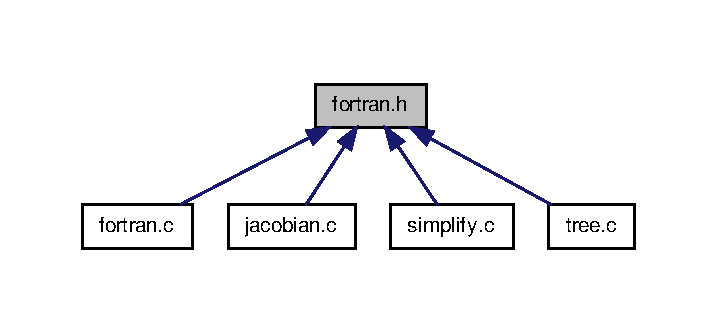
\includegraphics[width=344pt]{fortran_8h__dep__incl}
\end{center}
\end{figure}
\subsection*{Functions}
\begin{DoxyCompactItemize}
\item 
char $\ast$ \hyperlink{fortran_8h_a712ba008f0345618c5b1b87358a0206e}{to\-Fortran} (struct \hyperlink{structNode}{Node} $\ast$t)
\begin{DoxyCompactList}\small\item\em Recursively translate a Nodes to Fortran. \end{DoxyCompactList}\item 
void \hyperlink{fortran_8h_a2222da9d792b8540ffba7e25fbf4e4a4}{function\-To\-Fortran} (struct \hyperlink{structNode}{Node} $\ast$t)
\begin{DoxyCompactList}\small\item\em Translate a O\-D\-E function to Fortran. \end{DoxyCompactList}\item 
void \hyperlink{fortran_8h_a6d57af6f238f091e9c62b9ed81f194a3}{print\-Fortran\-Function} (struct \hyperlink{structNode}{Node} $\ast$t, int jac)
\begin{DoxyCompactList}\small\item\em Translate a O\-D\-E or Jacobian function to Fortran. \end{DoxyCompactList}\item 
char $\ast$ \hyperlink{fortran_8h_a9a1c3a7f211f7d42c6dedcdaed68067e}{line} (int label, char $\ast$content)
\begin{DoxyCompactList}\small\item\em Fit a string into the Fortran fixed format. \end{DoxyCompactList}\item 
char $\ast$ \hyperlink{fortran_8h_a02a98fd967252e6d807915856d09c77f}{F\-\_\-plus} (char $\ast$s1, char $\ast$s2)
\begin{DoxyCompactList}\small\item\em Generate Fortran code representing a plus (+) operation. \end{DoxyCompactList}\item 
char $\ast$ \hyperlink{fortran_8h_adc9b028cf89661eeb91182ab007da632}{F\-\_\-minus} (char $\ast$s1, char $\ast$s2)
\begin{DoxyCompactList}\small\item\em Generate Fortran code representing a minus (-\/) operation. \end{DoxyCompactList}\item 
char $\ast$ \hyperlink{fortran_8h_a0ca25a9453e2eeb469f1120368dd481f}{F\-\_\-negative} (char $\ast$s1)
\begin{DoxyCompactList}\small\item\em Generate Fortran code representing a negative sign (-\/) operation. \end{DoxyCompactList}\item 
char $\ast$ \hyperlink{fortran_8h_a1d67a9cba2734d4accc1f041aeab29dc}{F\-\_\-mul} (char $\ast$s1, char $\ast$s2)
\begin{DoxyCompactList}\small\item\em Generate Fortran code representing a multiplication ($\ast$) operation. \end{DoxyCompactList}\item 
char $\ast$ \hyperlink{fortran_8h_a0a05ea2fc6b0ca74871f60f1580fade0}{F\-\_\-div} (char $\ast$s1, char $\ast$s2)
\begin{DoxyCompactList}\small\item\em Generate Fortran code representing a division (/) operation. \end{DoxyCompactList}\item 
char $\ast$ \hyperlink{fortran_8h_ab1deef2cd69a27b35060de99428d6002}{F\-\_\-pow} (char $\ast$s1, char $\ast$s2)
\begin{DoxyCompactList}\small\item\em Generate Fortran code representing a power ($^\wedge$) operation. \end{DoxyCompactList}\item 
char $\ast$ \hyperlink{fortran_8h_ad039b3cb32f255dbab046b141de3b710}{F\-\_\-not} (char $\ast$s1)
\begin{DoxyCompactList}\small\item\em Generate Fortran code representing a N\-O\-T ($\sim$, !) operation. \end{DoxyCompactList}\item 
char $\ast$ \hyperlink{fortran_8h_a46ec6c338eb4bc765f191f1c4c3a4b53}{F\-\_\-eq\-\_\-op} (char $\ast$s1, char $\ast$s2)
\begin{DoxyCompactList}\small\item\em Generate Fortran code representing a E\-Q\-U\-A\-L (==) operation. \end{DoxyCompactList}\item 
char $\ast$ \hyperlink{fortran_8h_afaf4bf6f26417c1e1abb46f4a67b3d90}{F\-\_\-ne\-\_\-op} (char $\ast$s1, char $\ast$s2)
\begin{DoxyCompactList}\small\item\em Generate Fortran code representing a N\-O\-T E\-Q\-U\-A\-L ($\sim$=, !=) operation. \end{DoxyCompactList}\item 
char $\ast$ \hyperlink{fortran_8h_a97a8bc56d7ed7fee3bff400d1fd58ea3}{F\-\_\-gt\-\_\-op} (char $\ast$s1, char $\ast$s2)
\begin{DoxyCompactList}\small\item\em Generate Fortran code representing a G\-R\-E\-A\-T\-E\-R T\-H\-A\-N ($>$) operation. \end{DoxyCompactList}\item 
char $\ast$ \hyperlink{fortran_8h_ae69df0da134bdabf8e931d0f18f9a9de}{F\-\_\-ge\-\_\-op} (char $\ast$s1, char $\ast$s2)
\begin{DoxyCompactList}\small\item\em Generate Fortran code representing a G\-R\-E\-A\-T\-E\-R O\-R E\-Q\-U\-A\-L ($>$=) operation. \end{DoxyCompactList}\item 
char $\ast$ \hyperlink{fortran_8h_a168e6ceafab728511a2832d50e48942a}{F\-\_\-lt\-\_\-op} (char $\ast$s1, char $\ast$s2)
\begin{DoxyCompactList}\small\item\em Generate Fortran code representing a L\-E\-S\-S\-E\-R T\-H\-A\-N ($<$) operation. \end{DoxyCompactList}\item 
char $\ast$ \hyperlink{fortran_8h_a9b9a6759bf60f4ee7f53eb2af65acf05}{F\-\_\-le\-\_\-op} (char $\ast$s1, char $\ast$s2)
\begin{DoxyCompactList}\small\item\em Generate Fortran code representing a L\-E\-S\-S\-E\-R O\-R E\-Q\-U\-A\-L ($<$=) operation. \end{DoxyCompactList}\item 
char $\ast$ \hyperlink{fortran_8h_a3a9a87b9a8262532d796ae4904caac49}{F\-\_\-assign} (char $\ast$s1, char $\ast$s2)
\begin{DoxyCompactList}\small\item\em Generate Fortran code representing an assign (=) statement. \end{DoxyCompactList}\item 
char $\ast$ \hyperlink{fortran_8h_abafedd063906b6369ffadd0d9ec36f9e}{F\-\_\-for} (char $\ast$s1, char $\ast$s2, char $\ast$s3)
\begin{DoxyCompactList}\small\item\em Generate Fortran code representing a for statement. \end{DoxyCompactList}\item 
char $\ast$ \hyperlink{fortran_8h_aa6f504e52bf6b28f12fcb6f052642d04}{F\-\_\-range} (char $\ast$s1, char $\ast$s2, char $\ast$s3)
\begin{DoxyCompactList}\small\item\em Generate Fortran code representing a range (\-:) operation. \end{DoxyCompactList}\item 
char $\ast$ \hyperlink{fortran_8h_a6fc4168f0113431f451b2fbc8a23cd39}{F\-\_\-while} (char $\ast$s1, char $\ast$s2)
\begin{DoxyCompactList}\small\item\em Generate Fortran code representing a while statement. \end{DoxyCompactList}\item 
char $\ast$ \hyperlink{fortran_8h_a0cd8a485e5575fe231bd15bb724c904f}{F\-\_\-and} (char $\ast$s1, char $\ast$s2)
\begin{DoxyCompactList}\small\item\em Generate Fortran code representing an A\-N\-D (\&\&) operation. \end{DoxyCompactList}\item 
char $\ast$ \hyperlink{fortran_8h_a87a3641482ea51fff74931c9248ce245}{F\-\_\-or} (char $\ast$s1, char $\ast$s2)
\begin{DoxyCompactList}\small\item\em Generate Fortran code representing an O\-R ($|$$|$) operation. \end{DoxyCompactList}\item 
char $\ast$ \hyperlink{fortran_8h_ad35c68cadde4047a250fc7f3722cd4ba}{F\-\_\-if} (char $\ast$s1, char $\ast$s2)
\item 
char $\ast$ \hyperlink{fortran_8h_a9d12d2fadabc5cb43dcfd3da0a379a27}{F\-\_\-ifelse} (char $\ast$s1, char $\ast$s2, char $\ast$s3)
\item 
char $\ast$ \hyperlink{fortran_8h_aa40f8274e7e8d72e7bf45b8ba657b487}{F\-\_\-ifelseif} (char $\ast$s1, char $\ast$s2, char $\ast$s3)
\item 
char $\ast$ \hyperlink{fortran_8h_ae4f68d273f9c36127d05c8ce3036599e}{F\-\_\-elseif} (char $\ast$s1, char $\ast$s2)
\item 
char $\ast$ \hyperlink{fortran_8h_a3c18e2e40028988c33e5513716e00395}{F\-\_\-ifelseifelse} (char $\ast$s1, char $\ast$s2, char $\ast$s3, char $\ast$s4)
\item 
char $\ast$ \hyperlink{fortran_8h_abcfc636d10b338ba9603adc5080f8268}{F\-\_\-arrayindex} (char $\ast$s1, char $\ast$s2)
\begin{DoxyCompactList}\small\item\em Generate Fortran code representing an array indexing (a\mbox{[}b\mbox{]}) operation. \end{DoxyCompactList}\item 
char $\ast$ \hyperlink{fortran_8h_ae7130ea548b657055bbd08670caa7361}{F\-\_\-indexrange} (char $\ast$s1, char $\ast$s2)
\begin{DoxyCompactList}\small\item\em Generate Fortran code representing a range (\-:) operation. \end{DoxyCompactList}\item 
char $\ast$ \hyperlink{fortran_8h_ab230e89691dc4f8dff8d85472c20fd8a}{F\-\_\-zeros} (char $\ast$s1, char $\ast$s2, int allocate)
\item 
char $\ast$ \hyperlink{fortran_8h_a4193d629b89c1551beb365d1c0a4bc13}{F\-\_\-combine} (char $\ast$s1, char $\ast$s2)
\begin{DoxyCompactList}\small\item\em Generate Fortran code representing the subsequent execution of two statements. \end{DoxyCompactList}\end{DoxyCompactItemize}


\subsection{Function Documentation}
\hypertarget{fortran_8h_a0cd8a485e5575fe231bd15bb724c904f}{\index{fortran.\-h@{fortran.\-h}!F\-\_\-and@{F\-\_\-and}}
\index{F\-\_\-and@{F\-\_\-and}!fortran.h@{fortran.\-h}}
\subsubsection[{F\-\_\-and}]{\setlength{\rightskip}{0pt plus 5cm}char$\ast$ F\-\_\-and (
\begin{DoxyParamCaption}
\item[{char $\ast$}]{s1, }
\item[{char $\ast$}]{s2}
\end{DoxyParamCaption}
)}}\label{fortran_8h_a0cd8a485e5575fe231bd15bb724c904f}


Generate Fortran code representing an A\-N\-D (\&\&) operation. 

Generate Fortran code that applies an A\-N\-D (\&\&) operation on the code segments represented by {\itshape s1} and {\itshape s2} (s1 \&\& s2). 
\begin{DoxyParams}{Parameters}
{\em s1} & First code segment. \\
\hline
{\em s2} & Second code segment. \\
\hline
\end{DoxyParams}
\begin{DoxyReturn}{Returns}
The Fortran code. 
\end{DoxyReturn}
\hypertarget{fortran_8h_abcfc636d10b338ba9603adc5080f8268}{\index{fortran.\-h@{fortran.\-h}!F\-\_\-arrayindex@{F\-\_\-arrayindex}}
\index{F\-\_\-arrayindex@{F\-\_\-arrayindex}!fortran.h@{fortran.\-h}}
\subsubsection[{F\-\_\-arrayindex}]{\setlength{\rightskip}{0pt plus 5cm}char$\ast$ F\-\_\-arrayindex (
\begin{DoxyParamCaption}
\item[{char $\ast$}]{s1, }
\item[{char $\ast$}]{s2}
\end{DoxyParamCaption}
)}}\label{fortran_8h_abcfc636d10b338ba9603adc5080f8268}


Generate Fortran code representing an array indexing (a\mbox{[}b\mbox{]}) operation. 

Generate Fortran code that applies an array indexing (a\mbox{[}b\mbox{]}) operation on the code segments represented by {\itshape s1} and {\itshape s2} (s1\mbox{[}s2\mbox{]}). 
\begin{DoxyParams}{Parameters}
{\em s1} & First code segment. \\
\hline
{\em s2} & Second code segment. \\
\hline
\end{DoxyParams}
\begin{DoxyReturn}{Returns}
The Fortran code. 
\end{DoxyReturn}
\hypertarget{fortran_8h_a3a9a87b9a8262532d796ae4904caac49}{\index{fortran.\-h@{fortran.\-h}!F\-\_\-assign@{F\-\_\-assign}}
\index{F\-\_\-assign@{F\-\_\-assign}!fortran.h@{fortran.\-h}}
\subsubsection[{F\-\_\-assign}]{\setlength{\rightskip}{0pt plus 5cm}char$\ast$ F\-\_\-assign (
\begin{DoxyParamCaption}
\item[{char $\ast$}]{s1, }
\item[{char $\ast$}]{s2}
\end{DoxyParamCaption}
)}}\label{fortran_8h_a3a9a87b9a8262532d796ae4904caac49}


Generate Fortran code representing an assign (=) statement. 

Generate Fortran code that applies an assign (=) statement on the code segments represented by {\itshape s1} and {\itshape s2} (s1 = s2). 
\begin{DoxyParams}{Parameters}
{\em s1} & First code segment. \\
\hline
{\em s2} & Second code segment. \\
\hline
\end{DoxyParams}
\begin{DoxyReturn}{Returns}
The Fortran code. 
\end{DoxyReturn}
\hypertarget{fortran_8h_a4193d629b89c1551beb365d1c0a4bc13}{\index{fortran.\-h@{fortran.\-h}!F\-\_\-combine@{F\-\_\-combine}}
\index{F\-\_\-combine@{F\-\_\-combine}!fortran.h@{fortran.\-h}}
\subsubsection[{F\-\_\-combine}]{\setlength{\rightskip}{0pt plus 5cm}char$\ast$ F\-\_\-combine (
\begin{DoxyParamCaption}
\item[{char $\ast$}]{s1, }
\item[{char $\ast$}]{s2}
\end{DoxyParamCaption}
)}}\label{fortran_8h_a4193d629b89c1551beb365d1c0a4bc13}


Generate Fortran code representing the subsequent execution of two statements. 

Generate Fortran code that subsequently executes {\itshape s1} and {\itshape s2} (s1;s2). 
\begin{DoxyParams}{Parameters}
{\em s1} & First code segment. \\
\hline
{\em s2} & Second code segment. \\
\hline
\end{DoxyParams}
\begin{DoxyReturn}{Returns}
The Fortran code. 
\end{DoxyReturn}
\hypertarget{fortran_8h_a0a05ea2fc6b0ca74871f60f1580fade0}{\index{fortran.\-h@{fortran.\-h}!F\-\_\-div@{F\-\_\-div}}
\index{F\-\_\-div@{F\-\_\-div}!fortran.h@{fortran.\-h}}
\subsubsection[{F\-\_\-div}]{\setlength{\rightskip}{0pt plus 5cm}char$\ast$ F\-\_\-div (
\begin{DoxyParamCaption}
\item[{char $\ast$}]{s1, }
\item[{char $\ast$}]{s2}
\end{DoxyParamCaption}
)}}\label{fortran_8h_a0a05ea2fc6b0ca74871f60f1580fade0}


Generate Fortran code representing a division (/) operation. 

Generate Fortran code that applies a division (/) operation on the code segments represented by {\itshape s1} and {\itshape s2} (s1 / s2). 
\begin{DoxyParams}{Parameters}
{\em s1} & First code segment. \\
\hline
{\em s2} & Second code segment. \\
\hline
\end{DoxyParams}
\begin{DoxyReturn}{Returns}
The Fortran code. 
\end{DoxyReturn}
\hypertarget{fortran_8h_ae4f68d273f9c36127d05c8ce3036599e}{\index{fortran.\-h@{fortran.\-h}!F\-\_\-elseif@{F\-\_\-elseif}}
\index{F\-\_\-elseif@{F\-\_\-elseif}!fortran.h@{fortran.\-h}}
\subsubsection[{F\-\_\-elseif}]{\setlength{\rightskip}{0pt plus 5cm}char$\ast$ F\-\_\-elseif (
\begin{DoxyParamCaption}
\item[{char $\ast$}]{s1, }
\item[{char $\ast$}]{s2}
\end{DoxyParamCaption}
)}}\label{fortran_8h_ae4f68d273f9c36127d05c8ce3036599e}
\hypertarget{fortran_8h_a46ec6c338eb4bc765f191f1c4c3a4b53}{\index{fortran.\-h@{fortran.\-h}!F\-\_\-eq\-\_\-op@{F\-\_\-eq\-\_\-op}}
\index{F\-\_\-eq\-\_\-op@{F\-\_\-eq\-\_\-op}!fortran.h@{fortran.\-h}}
\subsubsection[{F\-\_\-eq\-\_\-op}]{\setlength{\rightskip}{0pt plus 5cm}char$\ast$ F\-\_\-eq\-\_\-op (
\begin{DoxyParamCaption}
\item[{char $\ast$}]{s1, }
\item[{char $\ast$}]{s2}
\end{DoxyParamCaption}
)}}\label{fortran_8h_a46ec6c338eb4bc765f191f1c4c3a4b53}


Generate Fortran code representing a E\-Q\-U\-A\-L (==) operation. 

Generate Fortran code that applies a E\-Q\-U\-A\-L (==) operation on the code segments represented by {\itshape s1} and {\itshape s2} (s1 == s2). 
\begin{DoxyParams}{Parameters}
{\em s1} & First code segment. \\
\hline
{\em s2} & Second code segment. \\
\hline
\end{DoxyParams}
\begin{DoxyReturn}{Returns}
The Fortran code. 
\end{DoxyReturn}
\hypertarget{fortran_8h_abafedd063906b6369ffadd0d9ec36f9e}{\index{fortran.\-h@{fortran.\-h}!F\-\_\-for@{F\-\_\-for}}
\index{F\-\_\-for@{F\-\_\-for}!fortran.h@{fortran.\-h}}
\subsubsection[{F\-\_\-for}]{\setlength{\rightskip}{0pt plus 5cm}char$\ast$ F\-\_\-for (
\begin{DoxyParamCaption}
\item[{char $\ast$}]{s1, }
\item[{char $\ast$}]{s2, }
\item[{char $\ast$}]{s3}
\end{DoxyParamCaption}
)}}\label{fortran_8h_abafedd063906b6369ffadd0d9ec36f9e}


Generate Fortran code representing a for statement. 

Generate Fortran code that applies a for statement on the code segments represented by {\itshape s1}, {\itshape s2} and {\itshape s3} (do {\itshape label} s1 = s2; s3; {\itshape label} continue). 
\begin{DoxyParams}{Parameters}
{\em s1} & First code segment. \\
\hline
{\em s2} & Second code segment. \\
\hline
{\em s3} & Third code segment. \\
\hline
\end{DoxyParams}
\begin{DoxyReturn}{Returns}
The Fortran code. 
\end{DoxyReturn}
\hypertarget{fortran_8h_ae69df0da134bdabf8e931d0f18f9a9de}{\index{fortran.\-h@{fortran.\-h}!F\-\_\-ge\-\_\-op@{F\-\_\-ge\-\_\-op}}
\index{F\-\_\-ge\-\_\-op@{F\-\_\-ge\-\_\-op}!fortran.h@{fortran.\-h}}
\subsubsection[{F\-\_\-ge\-\_\-op}]{\setlength{\rightskip}{0pt plus 5cm}char$\ast$ F\-\_\-ge\-\_\-op (
\begin{DoxyParamCaption}
\item[{char $\ast$}]{s1, }
\item[{char $\ast$}]{s2}
\end{DoxyParamCaption}
)}}\label{fortran_8h_ae69df0da134bdabf8e931d0f18f9a9de}


Generate Fortran code representing a G\-R\-E\-A\-T\-E\-R O\-R E\-Q\-U\-A\-L ($>$=) operation. 

Generate Fortran code that applies a G\-R\-E\-A\-T\-E\-R O\-R E\-Q\-U\-A\-L ($>$=) operation on the code segments represented by {\itshape s1} and {\itshape s2} (s1 $>$= s2). 
\begin{DoxyParams}{Parameters}
{\em s1} & First code segment. \\
\hline
{\em s2} & Second code segment. \\
\hline
\end{DoxyParams}
\begin{DoxyReturn}{Returns}
The Fortran code. 
\end{DoxyReturn}
\hypertarget{fortran_8h_a97a8bc56d7ed7fee3bff400d1fd58ea3}{\index{fortran.\-h@{fortran.\-h}!F\-\_\-gt\-\_\-op@{F\-\_\-gt\-\_\-op}}
\index{F\-\_\-gt\-\_\-op@{F\-\_\-gt\-\_\-op}!fortran.h@{fortran.\-h}}
\subsubsection[{F\-\_\-gt\-\_\-op}]{\setlength{\rightskip}{0pt plus 5cm}char$\ast$ F\-\_\-gt\-\_\-op (
\begin{DoxyParamCaption}
\item[{char $\ast$}]{s1, }
\item[{char $\ast$}]{s2}
\end{DoxyParamCaption}
)}}\label{fortran_8h_a97a8bc56d7ed7fee3bff400d1fd58ea3}


Generate Fortran code representing a G\-R\-E\-A\-T\-E\-R T\-H\-A\-N ($>$) operation. 

Generate Fortran code that applies a G\-R\-E\-A\-T\-E\-R T\-H\-A\-N ($>$) operation on the code segments represented by {\itshape s1} and {\itshape s2} (s1 $>$ s2). 
\begin{DoxyParams}{Parameters}
{\em s1} & First code segment. \\
\hline
{\em s2} & Second code segment. \\
\hline
\end{DoxyParams}
\begin{DoxyReturn}{Returns}
The Fortran code. 
\end{DoxyReturn}
\hypertarget{fortran_8h_ad35c68cadde4047a250fc7f3722cd4ba}{\index{fortran.\-h@{fortran.\-h}!F\-\_\-if@{F\-\_\-if}}
\index{F\-\_\-if@{F\-\_\-if}!fortran.h@{fortran.\-h}}
\subsubsection[{F\-\_\-if}]{\setlength{\rightskip}{0pt plus 5cm}char$\ast$ F\-\_\-if (
\begin{DoxyParamCaption}
\item[{char $\ast$}]{s1, }
\item[{char $\ast$}]{s2}
\end{DoxyParamCaption}
)}}\label{fortran_8h_ad35c68cadde4047a250fc7f3722cd4ba}
\hypertarget{fortran_8h_a9d12d2fadabc5cb43dcfd3da0a379a27}{\index{fortran.\-h@{fortran.\-h}!F\-\_\-ifelse@{F\-\_\-ifelse}}
\index{F\-\_\-ifelse@{F\-\_\-ifelse}!fortran.h@{fortran.\-h}}
\subsubsection[{F\-\_\-ifelse}]{\setlength{\rightskip}{0pt plus 5cm}char$\ast$ F\-\_\-ifelse (
\begin{DoxyParamCaption}
\item[{char $\ast$}]{s1, }
\item[{char $\ast$}]{s2, }
\item[{char $\ast$}]{s3}
\end{DoxyParamCaption}
)}}\label{fortran_8h_a9d12d2fadabc5cb43dcfd3da0a379a27}
\hypertarget{fortran_8h_aa40f8274e7e8d72e7bf45b8ba657b487}{\index{fortran.\-h@{fortran.\-h}!F\-\_\-ifelseif@{F\-\_\-ifelseif}}
\index{F\-\_\-ifelseif@{F\-\_\-ifelseif}!fortran.h@{fortran.\-h}}
\subsubsection[{F\-\_\-ifelseif}]{\setlength{\rightskip}{0pt plus 5cm}char$\ast$ F\-\_\-ifelseif (
\begin{DoxyParamCaption}
\item[{char $\ast$}]{s1, }
\item[{char $\ast$}]{s2, }
\item[{char $\ast$}]{s3}
\end{DoxyParamCaption}
)}}\label{fortran_8h_aa40f8274e7e8d72e7bf45b8ba657b487}
\hypertarget{fortran_8h_a3c18e2e40028988c33e5513716e00395}{\index{fortran.\-h@{fortran.\-h}!F\-\_\-ifelseifelse@{F\-\_\-ifelseifelse}}
\index{F\-\_\-ifelseifelse@{F\-\_\-ifelseifelse}!fortran.h@{fortran.\-h}}
\subsubsection[{F\-\_\-ifelseifelse}]{\setlength{\rightskip}{0pt plus 5cm}char$\ast$ F\-\_\-ifelseifelse (
\begin{DoxyParamCaption}
\item[{char $\ast$}]{s1, }
\item[{char $\ast$}]{s2, }
\item[{char $\ast$}]{s3, }
\item[{char $\ast$}]{s4}
\end{DoxyParamCaption}
)}}\label{fortran_8h_a3c18e2e40028988c33e5513716e00395}
\hypertarget{fortran_8h_ae7130ea548b657055bbd08670caa7361}{\index{fortran.\-h@{fortran.\-h}!F\-\_\-indexrange@{F\-\_\-indexrange}}
\index{F\-\_\-indexrange@{F\-\_\-indexrange}!fortran.h@{fortran.\-h}}
\subsubsection[{F\-\_\-indexrange}]{\setlength{\rightskip}{0pt plus 5cm}char$\ast$ F\-\_\-indexrange (
\begin{DoxyParamCaption}
\item[{char $\ast$}]{s1, }
\item[{char $\ast$}]{s2}
\end{DoxyParamCaption}
)}}\label{fortran_8h_ae7130ea548b657055bbd08670caa7361}


Generate Fortran code representing a range (\-:) operation. 

Generate Fortran code that applies a range (\-:) operation on the code segments represented by {\itshape s1} and {\itshape s2} preparing it for use in an array indexing expression (s1\-:s2). 
\begin{DoxyParams}{Parameters}
{\em s1} & First code segment. \\
\hline
{\em s2} & Second code segment. \\
\hline
\end{DoxyParams}
\begin{DoxyReturn}{Returns}
The Fortran code. 
\end{DoxyReturn}
\hypertarget{fortran_8h_a9b9a6759bf60f4ee7f53eb2af65acf05}{\index{fortran.\-h@{fortran.\-h}!F\-\_\-le\-\_\-op@{F\-\_\-le\-\_\-op}}
\index{F\-\_\-le\-\_\-op@{F\-\_\-le\-\_\-op}!fortran.h@{fortran.\-h}}
\subsubsection[{F\-\_\-le\-\_\-op}]{\setlength{\rightskip}{0pt plus 5cm}char$\ast$ F\-\_\-le\-\_\-op (
\begin{DoxyParamCaption}
\item[{char $\ast$}]{s1, }
\item[{char $\ast$}]{s2}
\end{DoxyParamCaption}
)}}\label{fortran_8h_a9b9a6759bf60f4ee7f53eb2af65acf05}


Generate Fortran code representing a L\-E\-S\-S\-E\-R O\-R E\-Q\-U\-A\-L ($<$=) operation. 

Generate Fortran code that applies a L\-E\-S\-S\-E\-R O\-R E\-Q\-U\-A\-L ($<$=) operation on the code segments represented by {\itshape s1} and {\itshape s2} (s1 $<$= s2). 
\begin{DoxyParams}{Parameters}
{\em s1} & First code segment. \\
\hline
{\em s2} & Second code segment. \\
\hline
\end{DoxyParams}
\begin{DoxyReturn}{Returns}
The Fortran code. 
\end{DoxyReturn}
\hypertarget{fortran_8h_a168e6ceafab728511a2832d50e48942a}{\index{fortran.\-h@{fortran.\-h}!F\-\_\-lt\-\_\-op@{F\-\_\-lt\-\_\-op}}
\index{F\-\_\-lt\-\_\-op@{F\-\_\-lt\-\_\-op}!fortran.h@{fortran.\-h}}
\subsubsection[{F\-\_\-lt\-\_\-op}]{\setlength{\rightskip}{0pt plus 5cm}char$\ast$ F\-\_\-lt\-\_\-op (
\begin{DoxyParamCaption}
\item[{char $\ast$}]{s1, }
\item[{char $\ast$}]{s2}
\end{DoxyParamCaption}
)}}\label{fortran_8h_a168e6ceafab728511a2832d50e48942a}


Generate Fortran code representing a L\-E\-S\-S\-E\-R T\-H\-A\-N ($<$) operation. 

Generate Fortran code that applies a L\-E\-S\-S\-E\-R T\-H\-A\-N ($<$) operation on the code segments represented by {\itshape s1} and {\itshape s2} (s1 $<$= s2). 
\begin{DoxyParams}{Parameters}
{\em s1} & First code segment. \\
\hline
{\em s2} & Second code segment. \\
\hline
\end{DoxyParams}
\begin{DoxyReturn}{Returns}
The Fortran code. 
\end{DoxyReturn}
\hypertarget{fortran_8h_adc9b028cf89661eeb91182ab007da632}{\index{fortran.\-h@{fortran.\-h}!F\-\_\-minus@{F\-\_\-minus}}
\index{F\-\_\-minus@{F\-\_\-minus}!fortran.h@{fortran.\-h}}
\subsubsection[{F\-\_\-minus}]{\setlength{\rightskip}{0pt plus 5cm}char$\ast$ F\-\_\-minus (
\begin{DoxyParamCaption}
\item[{char $\ast$}]{s1, }
\item[{char $\ast$}]{s2}
\end{DoxyParamCaption}
)}}\label{fortran_8h_adc9b028cf89661eeb91182ab007da632}


Generate Fortran code representing a minus (-\/) operation. 

Generate Fortran code that applies a minus (-\/) operation on the code segments represented by {\itshape s1} and {\itshape s2} (s1 -\/ s2). 
\begin{DoxyParams}{Parameters}
{\em s1} & First code segment. \\
\hline
{\em s2} & Second code segment. \\
\hline
\end{DoxyParams}
\begin{DoxyReturn}{Returns}
The Fortran code. 
\end{DoxyReturn}
\hypertarget{fortran_8h_a1d67a9cba2734d4accc1f041aeab29dc}{\index{fortran.\-h@{fortran.\-h}!F\-\_\-mul@{F\-\_\-mul}}
\index{F\-\_\-mul@{F\-\_\-mul}!fortran.h@{fortran.\-h}}
\subsubsection[{F\-\_\-mul}]{\setlength{\rightskip}{0pt plus 5cm}char$\ast$ F\-\_\-mul (
\begin{DoxyParamCaption}
\item[{char $\ast$}]{s1, }
\item[{char $\ast$}]{s2}
\end{DoxyParamCaption}
)}}\label{fortran_8h_a1d67a9cba2734d4accc1f041aeab29dc}


Generate Fortran code representing a multiplication ($\ast$) operation. 

Generate Fortran code that applies a multiplication ($\ast$) operation on the code segments represented by {\itshape s1} and {\itshape s2} (s1 $\ast$ s2). 
\begin{DoxyParams}{Parameters}
{\em s1} & First code segment. \\
\hline
{\em s2} & Second code segment. \\
\hline
\end{DoxyParams}
\begin{DoxyReturn}{Returns}
The Fortran code. 
\end{DoxyReturn}
\hypertarget{fortran_8h_afaf4bf6f26417c1e1abb46f4a67b3d90}{\index{fortran.\-h@{fortran.\-h}!F\-\_\-ne\-\_\-op@{F\-\_\-ne\-\_\-op}}
\index{F\-\_\-ne\-\_\-op@{F\-\_\-ne\-\_\-op}!fortran.h@{fortran.\-h}}
\subsubsection[{F\-\_\-ne\-\_\-op}]{\setlength{\rightskip}{0pt plus 5cm}char$\ast$ F\-\_\-ne\-\_\-op (
\begin{DoxyParamCaption}
\item[{char $\ast$}]{s1, }
\item[{char $\ast$}]{s2}
\end{DoxyParamCaption}
)}}\label{fortran_8h_afaf4bf6f26417c1e1abb46f4a67b3d90}


Generate Fortran code representing a N\-O\-T E\-Q\-U\-A\-L ($\sim$=, !=) operation. 

Generate Fortran code that applies a N\-O\-T E\-Q\-U\-A\-L ($\sim$=, !=) operation on the code segments represented by {\itshape s1} and {\itshape s2} (s1 != s2). 
\begin{DoxyParams}{Parameters}
{\em s1} & First code segment. \\
\hline
{\em s2} & Second code segment. \\
\hline
\end{DoxyParams}
\begin{DoxyReturn}{Returns}
The Fortran code. 
\end{DoxyReturn}
\hypertarget{fortran_8h_a0ca25a9453e2eeb469f1120368dd481f}{\index{fortran.\-h@{fortran.\-h}!F\-\_\-negative@{F\-\_\-negative}}
\index{F\-\_\-negative@{F\-\_\-negative}!fortran.h@{fortran.\-h}}
\subsubsection[{F\-\_\-negative}]{\setlength{\rightskip}{0pt plus 5cm}char$\ast$ F\-\_\-negative (
\begin{DoxyParamCaption}
\item[{char $\ast$}]{s1}
\end{DoxyParamCaption}
)}}\label{fortran_8h_a0ca25a9453e2eeb469f1120368dd481f}


Generate Fortran code representing a negative sign (-\/) operation. 

Generate Fortran code that applies a negative sign (-\/) operation on the code segment represented by {\itshape s1} (-\/s1). 
\begin{DoxyParams}{Parameters}
{\em s1} & Code segment. \\
\hline
\end{DoxyParams}
\begin{DoxyReturn}{Returns}
The Fortran code. 
\end{DoxyReturn}
\hypertarget{fortran_8h_ad039b3cb32f255dbab046b141de3b710}{\index{fortran.\-h@{fortran.\-h}!F\-\_\-not@{F\-\_\-not}}
\index{F\-\_\-not@{F\-\_\-not}!fortran.h@{fortran.\-h}}
\subsubsection[{F\-\_\-not}]{\setlength{\rightskip}{0pt plus 5cm}char$\ast$ F\-\_\-not (
\begin{DoxyParamCaption}
\item[{char $\ast$}]{s1}
\end{DoxyParamCaption}
)}}\label{fortran_8h_ad039b3cb32f255dbab046b141de3b710}


Generate Fortran code representing a N\-O\-T ($\sim$, !) operation. 

Generate Fortran code that applies a N\-O\-T ($\sim$, !) operation on the code segment represented by {\itshape s1} ($\sim$s1, !s1). 
\begin{DoxyParams}{Parameters}
{\em s1} & Code segment. \\
\hline
\end{DoxyParams}
\begin{DoxyReturn}{Returns}
The Fortran code. 
\end{DoxyReturn}
\hypertarget{fortran_8h_a87a3641482ea51fff74931c9248ce245}{\index{fortran.\-h@{fortran.\-h}!F\-\_\-or@{F\-\_\-or}}
\index{F\-\_\-or@{F\-\_\-or}!fortran.h@{fortran.\-h}}
\subsubsection[{F\-\_\-or}]{\setlength{\rightskip}{0pt plus 5cm}char$\ast$ F\-\_\-or (
\begin{DoxyParamCaption}
\item[{char $\ast$}]{s1, }
\item[{char $\ast$}]{s2}
\end{DoxyParamCaption}
)}}\label{fortran_8h_a87a3641482ea51fff74931c9248ce245}


Generate Fortran code representing an O\-R ($|$$|$) operation. 

Generate Fortran code that applies an O\-R ($|$$|$) operation on the code segments represented by {\itshape s1} and {\itshape s2} (s1 \&\& s2). 
\begin{DoxyParams}{Parameters}
{\em s1} & First code segment. \\
\hline
{\em s2} & Second code segment. \\
\hline
\end{DoxyParams}
\begin{DoxyReturn}{Returns}
The Fortran code. 
\end{DoxyReturn}
\hypertarget{fortran_8h_a02a98fd967252e6d807915856d09c77f}{\index{fortran.\-h@{fortran.\-h}!F\-\_\-plus@{F\-\_\-plus}}
\index{F\-\_\-plus@{F\-\_\-plus}!fortran.h@{fortran.\-h}}
\subsubsection[{F\-\_\-plus}]{\setlength{\rightskip}{0pt plus 5cm}char$\ast$ F\-\_\-plus (
\begin{DoxyParamCaption}
\item[{char $\ast$}]{s1, }
\item[{char $\ast$}]{s2}
\end{DoxyParamCaption}
)}}\label{fortran_8h_a02a98fd967252e6d807915856d09c77f}


Generate Fortran code representing a plus (+) operation. 

Generate Fortran code that applies a plus (+) operation on the code segments represented by {\itshape s1} and {\itshape s2} (s1 + s2). 
\begin{DoxyParams}{Parameters}
{\em s1} & First code segment. \\
\hline
{\em s2} & Second code segment. \\
\hline
\end{DoxyParams}
\begin{DoxyReturn}{Returns}
The Fortran code. 
\end{DoxyReturn}
\hypertarget{fortran_8h_ab1deef2cd69a27b35060de99428d6002}{\index{fortran.\-h@{fortran.\-h}!F\-\_\-pow@{F\-\_\-pow}}
\index{F\-\_\-pow@{F\-\_\-pow}!fortran.h@{fortran.\-h}}
\subsubsection[{F\-\_\-pow}]{\setlength{\rightskip}{0pt plus 5cm}char$\ast$ F\-\_\-pow (
\begin{DoxyParamCaption}
\item[{char $\ast$}]{s1, }
\item[{char $\ast$}]{s2}
\end{DoxyParamCaption}
)}}\label{fortran_8h_ab1deef2cd69a27b35060de99428d6002}


Generate Fortran code representing a power ($^\wedge$) operation. 

Generate Fortran code that applies a power ($^\wedge$) operation on the code segments represented by {\itshape s1} and {\itshape s2} (s1$^\wedge$s2). 
\begin{DoxyParams}{Parameters}
{\em s1} & First code segment. \\
\hline
{\em s2} & Second code segment. \\
\hline
\end{DoxyParams}
\begin{DoxyReturn}{Returns}
The Fortran code. 
\end{DoxyReturn}
\hypertarget{fortran_8h_aa6f504e52bf6b28f12fcb6f052642d04}{\index{fortran.\-h@{fortran.\-h}!F\-\_\-range@{F\-\_\-range}}
\index{F\-\_\-range@{F\-\_\-range}!fortran.h@{fortran.\-h}}
\subsubsection[{F\-\_\-range}]{\setlength{\rightskip}{0pt plus 5cm}char$\ast$ F\-\_\-range (
\begin{DoxyParamCaption}
\item[{char $\ast$}]{s1, }
\item[{char $\ast$}]{s2, }
\item[{char $\ast$}]{s3}
\end{DoxyParamCaption}
)}}\label{fortran_8h_aa6f504e52bf6b28f12fcb6f052642d04}


Generate Fortran code representing a range (\-:) operation. 

Generate Fortran code that applies a range (\-:) operation on the code segments represented by {\itshape s1}, {\itshape s2} and {\itshape s3}, preparing it for use in a for/do loop. 
\begin{DoxyParams}{Parameters}
{\em s1} & First code segment. \\
\hline
{\em s2} & Second code segment. \\
\hline
{\em s3} & Second code segment. \\
\hline
\end{DoxyParams}
\begin{DoxyReturn}{Returns}
The Fortran code. 
\end{DoxyReturn}
\hypertarget{fortran_8h_a6fc4168f0113431f451b2fbc8a23cd39}{\index{fortran.\-h@{fortran.\-h}!F\-\_\-while@{F\-\_\-while}}
\index{F\-\_\-while@{F\-\_\-while}!fortran.h@{fortran.\-h}}
\subsubsection[{F\-\_\-while}]{\setlength{\rightskip}{0pt plus 5cm}char$\ast$ F\-\_\-while (
\begin{DoxyParamCaption}
\item[{char $\ast$}]{s1, }
\item[{char $\ast$}]{s2}
\end{DoxyParamCaption}
)}}\label{fortran_8h_a6fc4168f0113431f451b2fbc8a23cd39}


Generate Fortran code representing a while statement. 

Generate Fortran code that applies a while statement on the code segments represented by {\itshape s1} and {\itshape s2} (while (s1); s2; end while). 
\begin{DoxyParams}{Parameters}
{\em s1} & First code segment. \\
\hline
{\em s2} & Second code segment. \\
\hline
\end{DoxyParams}
\begin{DoxyReturn}{Returns}
The Fortran code. 
\end{DoxyReturn}
\hypertarget{fortran_8h_ab230e89691dc4f8dff8d85472c20fd8a}{\index{fortran.\-h@{fortran.\-h}!F\-\_\-zeros@{F\-\_\-zeros}}
\index{F\-\_\-zeros@{F\-\_\-zeros}!fortran.h@{fortran.\-h}}
\subsubsection[{F\-\_\-zeros}]{\setlength{\rightskip}{0pt plus 5cm}char$\ast$ F\-\_\-zeros (
\begin{DoxyParamCaption}
\item[{char $\ast$}]{s1, }
\item[{char $\ast$}]{s2, }
\item[{int}]{allocate}
\end{DoxyParamCaption}
)}}\label{fortran_8h_ab230e89691dc4f8dff8d85472c20fd8a}
\hypertarget{fortran_8h_a2222da9d792b8540ffba7e25fbf4e4a4}{\index{fortran.\-h@{fortran.\-h}!function\-To\-Fortran@{function\-To\-Fortran}}
\index{function\-To\-Fortran@{function\-To\-Fortran}!fortran.h@{fortran.\-h}}
\subsubsection[{function\-To\-Fortran}]{\setlength{\rightskip}{0pt plus 5cm}void function\-To\-Fortran (
\begin{DoxyParamCaption}
\item[{struct {\bf Node} $\ast$}]{t}
\end{DoxyParamCaption}
)}}\label{fortran_8h_a2222da9d792b8540ffba7e25fbf4e4a4}


Translate a O\-D\-E function to Fortran. 

Recursively translate the O\-D\-E function represented by {\itshape t} to Fortran and print the generated code to the output stream \hyperlink{tree_8h_a1277960b5f2b37137fe9b0b5a1ea0beb}{out}. 
\begin{DoxyParams}{Parameters}
{\em t} & O\-D\-E function to translate. \\
\hline
\end{DoxyParams}
\hypertarget{fortran_8h_a9a1c3a7f211f7d42c6dedcdaed68067e}{\index{fortran.\-h@{fortran.\-h}!line@{line}}
\index{line@{line}!fortran.h@{fortran.\-h}}
\subsubsection[{line}]{\setlength{\rightskip}{0pt plus 5cm}char$\ast$ line (
\begin{DoxyParamCaption}
\item[{int}]{label, }
\item[{char $\ast$}]{content}
\end{DoxyParamCaption}
)}}\label{fortran_8h_a9a1c3a7f211f7d42c6dedcdaed68067e}


Fit a string into the Fortran fixed format. 

Generates a Fortran fixed format output by distributing the {\itshape content} over multiple lines if lines would exceed the 72 characters allowed by this format. Furthermore the function takes care of the first six control characters. A label will be added if {\itshape label} is not equal to zero. 
\begin{DoxyParams}{Parameters}
{\em label} & Label to add to the line. 0 for no label. \\
\hline
{\em content} & Actual code that should be fit into the format. \\
\hline
\end{DoxyParams}
\begin{DoxyReturn}{Returns}
The fixed form of the code provided. 
\end{DoxyReturn}
\hypertarget{fortran_8h_a6d57af6f238f091e9c62b9ed81f194a3}{\index{fortran.\-h@{fortran.\-h}!print\-Fortran\-Function@{print\-Fortran\-Function}}
\index{print\-Fortran\-Function@{print\-Fortran\-Function}!fortran.h@{fortran.\-h}}
\subsubsection[{print\-Fortran\-Function}]{\setlength{\rightskip}{0pt plus 5cm}void print\-Fortran\-Function (
\begin{DoxyParamCaption}
\item[{struct {\bf Node} $\ast$}]{t, }
\item[{int}]{jac}
\end{DoxyParamCaption}
)}}\label{fortran_8h_a6d57af6f238f091e9c62b9ed81f194a3}


Translate a O\-D\-E or Jacobian function to Fortran. 

Recursively translate the O\-D\-E or Jacobian function represented by {\itshape t} to Fortran and print the generated code to the output stream \hyperlink{tree_8h_a1277960b5f2b37137fe9b0b5a1ea0beb}{out}. {\itshape jac} should be 0 for O\-D\-E functions and 1 for Jacobian functions. 
\begin{DoxyParams}{Parameters}
{\em t} & \hyperlink{structFunction}{Function} to translate. \\
\hline
{\em jac} & Whether the function is a O\-D\-E (0) or Jacobian (1) function. \\
\hline
\end{DoxyParams}
\hypertarget{fortran_8h_a712ba008f0345618c5b1b87358a0206e}{\index{fortran.\-h@{fortran.\-h}!to\-Fortran@{to\-Fortran}}
\index{to\-Fortran@{to\-Fortran}!fortran.h@{fortran.\-h}}
\subsubsection[{to\-Fortran}]{\setlength{\rightskip}{0pt plus 5cm}char$\ast$ to\-Fortran (
\begin{DoxyParamCaption}
\item[{struct {\bf Node} $\ast$}]{t}
\end{DoxyParamCaption}
)}}\label{fortran_8h_a712ba008f0345618c5b1b87358a0206e}


Recursively translate a Nodes to Fortran. 

Translate \hyperlink{structNode}{Node} {\itshape t} to fixed format Fortran 95 code and do the same for its children. 
\begin{DoxyParams}{Parameters}
{\em t} & \hyperlink{structNode}{Node} to translate. \\
\hline
\end{DoxyParams}
\begin{DoxyReturn}{Returns}
String of Fortran code. 
\end{DoxyReturn}

\hypertarget{jacobian_8c}{\section{jacobian.\-c File Reference}
\label{jacobian_8c}\index{jacobian.\-c@{jacobian.\-c}}
}
{\ttfamily \#include $<$stdio.\-h$>$}\\*
{\ttfamily \#include $<$stdlib.\-h$>$}\\*
{\ttfamily \#include $<$string.\-h$>$}\\*
{\ttfamily \#include \char`\"{}jacobian.\-h\char`\"{}}\\*
{\ttfamily \#include \char`\"{}simplify.\-h\char`\"{}}\\*
{\ttfamily \#include \char`\"{}fortran.\-h\char`\"{}}\\*
{\ttfamily \#include \char`\"{}tree.\-h\char`\"{}}\\*
{\ttfamily \#include \char`\"{}node.\-h\char`\"{}}\\*
Include dependency graph for jacobian.\-c\-:\nopagebreak
\begin{figure}[H]
\begin{center}
\leavevmode
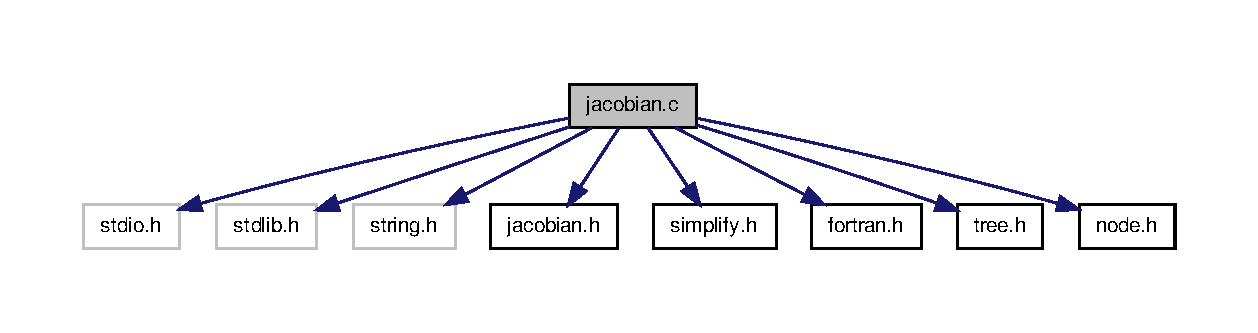
\includegraphics[width=350pt]{jacobian_8c__incl}
\end{center}
\end{figure}
\subsection*{Macros}
\begin{DoxyCompactItemize}
\item 
\#define \hyperlink{jacobian_8c_a369266c24eacffb87046522897a570d5}{\-\_\-\-G\-N\-U\-\_\-\-S\-O\-U\-R\-C\-E}
\end{DoxyCompactItemize}
\subsection*{Functions}
\begin{DoxyCompactItemize}
\item 
char $\ast$ \hyperlink{jacobian_8c_a21d0cae9ba0f71cac6989332790340a4}{D} (char $\ast$name)
\item 
void \hyperlink{jacobian_8c_a63b2497734bd2aea0c2648ee592913ae}{function\-To\-Jacobian} (struct \hyperlink{structNode}{Node} $\ast$t)
\item 
struct \hyperlink{structNode}{Node} $\ast$ \hyperlink{jacobian_8c_a679e6863209bf428a60f209b8ac64b2f}{derivative} (struct \hyperlink{structNode}{Node} $\ast$n, struct \hyperlink{structNode}{Node} $\ast$j)
\item 
struct \hyperlink{structNode}{Node} $\ast$ \hyperlink{jacobian_8c_a9a73fec39d6f63181e0718e5af7a4580}{D\-\_\-zeros} (char $\ast$iden, struct \hyperlink{structNode}{Node} $\ast$n)
\item 
struct \hyperlink{structNode}{Node} $\ast$ \hyperlink{jacobian_8c_a7709640e1a5d9fdbe4b02d07e1389848}{D\-\_\-plus} (struct \hyperlink{structNode}{Node} $\ast$n1, struct \hyperlink{structNode}{Node} $\ast$n2, struct \hyperlink{structNode}{Node} $\ast$j)
\item 
struct \hyperlink{structNode}{Node} $\ast$ \hyperlink{jacobian_8c_a18e1538e30dfe1e4d675c9ae7e090912}{D\-\_\-minus} (struct \hyperlink{structNode}{Node} $\ast$n1, struct \hyperlink{structNode}{Node} $\ast$n2, struct \hyperlink{structNode}{Node} $\ast$j)
\item 
struct \hyperlink{structNode}{Node} $\ast$ \hyperlink{jacobian_8c_aabf319e76dcbd7f0f8135daea08130fb}{D\-\_\-negative} (struct \hyperlink{structNode}{Node} $\ast$n1, struct \hyperlink{structNode}{Node} $\ast$j)
\item 
struct \hyperlink{structNode}{Node} $\ast$ \hyperlink{jacobian_8c_a563b2d2ddf25802728e25a796247e051}{D\-\_\-mul} (struct \hyperlink{structNode}{Node} $\ast$n1, struct \hyperlink{structNode}{Node} $\ast$n2, struct \hyperlink{structNode}{Node} $\ast$j)
\item 
struct \hyperlink{structNode}{Node} $\ast$ \hyperlink{jacobian_8c_a7a5c37c4ee6200ad5b2ed80f44594f7d}{D\-\_\-div} (struct \hyperlink{structNode}{Node} $\ast$n1, struct \hyperlink{structNode}{Node} $\ast$n2, struct \hyperlink{structNode}{Node} $\ast$j)
\item 
struct \hyperlink{structNode}{Node} $\ast$ \hyperlink{jacobian_8c_ac69adbac2f1488631e322c8541d15c74}{D\-\_\-pow} (struct \hyperlink{structNode}{Node} $\ast$n1, struct \hyperlink{structNode}{Node} $\ast$n2, struct \hyperlink{structNode}{Node} $\ast$j)
\item 
struct \hyperlink{structNode}{Node} $\ast$ \hyperlink{jacobian_8c_adcb98e7d3dc6a9f4a69b2444a02ffc51}{D\-\_\-var} (struct \hyperlink{structNode}{Node} $\ast$n)
\item 
struct \hyperlink{structNode}{Node} $\ast$ \hyperlink{jacobian_8c_af7f82a4a6c2a7751ae8b1ddfeda4c7e7}{D\-\_\-assign} (struct \hyperlink{structNode}{Node} $\ast$n1, struct \hyperlink{structNode}{Node} $\ast$n2)
\item 
struct \hyperlink{structNode}{Node} $\ast$ \hyperlink{jacobian_8c_a39e38e4c1369d762f09f15c5e4e727a1}{D\-\_\-if} (struct \hyperlink{structNode}{Node} $\ast$n1, struct \hyperlink{structNode}{Node} $\ast$n2, struct \hyperlink{structNode}{Node} $\ast$j)
\item 
struct \hyperlink{structNode}{Node} $\ast$ \hyperlink{jacobian_8c_a66841a427a1ef221a92813ab9980933c}{D\-\_\-ifelse} (struct \hyperlink{structNode}{Node} $\ast$n1, struct \hyperlink{structNode}{Node} $\ast$n2, struct \hyperlink{structNode}{Node} $\ast$n3, struct \hyperlink{structNode}{Node} $\ast$j)
\item 
struct \hyperlink{structNode}{Node} $\ast$ \hyperlink{jacobian_8c_a5d2292d7cc66b8ab6bf756608e0e2b7a}{D\-\_\-arrayindex} (char $\ast$iden, struct \hyperlink{structNode}{Node} $\ast$n)
\item 
struct \hyperlink{structNode}{Node} $\ast$ \hyperlink{jacobian_8c_aa5e579b47c173b8044d76eaefe0f0ecf}{D\-\_\-for} (char $\ast$iden, struct \hyperlink{structNode}{Node} $\ast$n1, struct \hyperlink{structNode}{Node} $\ast$n2)
\end{DoxyCompactItemize}


\subsection{Macro Definition Documentation}
\hypertarget{jacobian_8c_a369266c24eacffb87046522897a570d5}{\index{jacobian.\-c@{jacobian.\-c}!\-\_\-\-G\-N\-U\-\_\-\-S\-O\-U\-R\-C\-E@{\-\_\-\-G\-N\-U\-\_\-\-S\-O\-U\-R\-C\-E}}
\index{\-\_\-\-G\-N\-U\-\_\-\-S\-O\-U\-R\-C\-E@{\-\_\-\-G\-N\-U\-\_\-\-S\-O\-U\-R\-C\-E}!jacobian.c@{jacobian.\-c}}
\subsubsection[{\-\_\-\-G\-N\-U\-\_\-\-S\-O\-U\-R\-C\-E}]{\setlength{\rightskip}{0pt plus 5cm}\#define \-\_\-\-G\-N\-U\-\_\-\-S\-O\-U\-R\-C\-E}}\label{jacobian_8c_a369266c24eacffb87046522897a570d5}


\subsection{Function Documentation}
\hypertarget{jacobian_8c_a21d0cae9ba0f71cac6989332790340a4}{\index{jacobian.\-c@{jacobian.\-c}!D@{D}}
\index{D@{D}!jacobian.c@{jacobian.\-c}}
\subsubsection[{D}]{\setlength{\rightskip}{0pt plus 5cm}char$\ast$ D (
\begin{DoxyParamCaption}
\item[{char $\ast$}]{name}
\end{DoxyParamCaption}
)}}\label{jacobian_8c_a21d0cae9ba0f71cac6989332790340a4}
\hypertarget{jacobian_8c_a5d2292d7cc66b8ab6bf756608e0e2b7a}{\index{jacobian.\-c@{jacobian.\-c}!D\-\_\-arrayindex@{D\-\_\-arrayindex}}
\index{D\-\_\-arrayindex@{D\-\_\-arrayindex}!jacobian.c@{jacobian.\-c}}
\subsubsection[{D\-\_\-arrayindex}]{\setlength{\rightskip}{0pt plus 5cm}struct {\bf Node}$\ast$ D\-\_\-arrayindex (
\begin{DoxyParamCaption}
\item[{char $\ast$}]{iden, }
\item[{struct {\bf Node} $\ast$}]{n}
\end{DoxyParamCaption}
)}}\label{jacobian_8c_a5d2292d7cc66b8ab6bf756608e0e2b7a}
\hypertarget{jacobian_8c_af7f82a4a6c2a7751ae8b1ddfeda4c7e7}{\index{jacobian.\-c@{jacobian.\-c}!D\-\_\-assign@{D\-\_\-assign}}
\index{D\-\_\-assign@{D\-\_\-assign}!jacobian.c@{jacobian.\-c}}
\subsubsection[{D\-\_\-assign}]{\setlength{\rightskip}{0pt plus 5cm}struct {\bf Node}$\ast$ D\-\_\-assign (
\begin{DoxyParamCaption}
\item[{struct {\bf Node} $\ast$}]{n1, }
\item[{struct {\bf Node} $\ast$}]{n2}
\end{DoxyParamCaption}
)}}\label{jacobian_8c_af7f82a4a6c2a7751ae8b1ddfeda4c7e7}
\hypertarget{jacobian_8c_a7a5c37c4ee6200ad5b2ed80f44594f7d}{\index{jacobian.\-c@{jacobian.\-c}!D\-\_\-div@{D\-\_\-div}}
\index{D\-\_\-div@{D\-\_\-div}!jacobian.c@{jacobian.\-c}}
\subsubsection[{D\-\_\-div}]{\setlength{\rightskip}{0pt plus 5cm}struct {\bf Node}$\ast$ D\-\_\-div (
\begin{DoxyParamCaption}
\item[{struct {\bf Node} $\ast$}]{n1, }
\item[{struct {\bf Node} $\ast$}]{n2, }
\item[{struct {\bf Node} $\ast$}]{j}
\end{DoxyParamCaption}
)}}\label{jacobian_8c_a7a5c37c4ee6200ad5b2ed80f44594f7d}
\hypertarget{jacobian_8c_aa5e579b47c173b8044d76eaefe0f0ecf}{\index{jacobian.\-c@{jacobian.\-c}!D\-\_\-for@{D\-\_\-for}}
\index{D\-\_\-for@{D\-\_\-for}!jacobian.c@{jacobian.\-c}}
\subsubsection[{D\-\_\-for}]{\setlength{\rightskip}{0pt plus 5cm}struct {\bf Node}$\ast$ D\-\_\-for (
\begin{DoxyParamCaption}
\item[{char $\ast$}]{iden, }
\item[{struct {\bf Node} $\ast$}]{n1, }
\item[{struct {\bf Node} $\ast$}]{n2}
\end{DoxyParamCaption}
)}}\label{jacobian_8c_aa5e579b47c173b8044d76eaefe0f0ecf}
\hypertarget{jacobian_8c_a39e38e4c1369d762f09f15c5e4e727a1}{\index{jacobian.\-c@{jacobian.\-c}!D\-\_\-if@{D\-\_\-if}}
\index{D\-\_\-if@{D\-\_\-if}!jacobian.c@{jacobian.\-c}}
\subsubsection[{D\-\_\-if}]{\setlength{\rightskip}{0pt plus 5cm}struct {\bf Node}$\ast$ D\-\_\-if (
\begin{DoxyParamCaption}
\item[{struct {\bf Node} $\ast$}]{n1, }
\item[{struct {\bf Node} $\ast$}]{n2, }
\item[{struct {\bf Node} $\ast$}]{j}
\end{DoxyParamCaption}
)}}\label{jacobian_8c_a39e38e4c1369d762f09f15c5e4e727a1}
\hypertarget{jacobian_8c_a66841a427a1ef221a92813ab9980933c}{\index{jacobian.\-c@{jacobian.\-c}!D\-\_\-ifelse@{D\-\_\-ifelse}}
\index{D\-\_\-ifelse@{D\-\_\-ifelse}!jacobian.c@{jacobian.\-c}}
\subsubsection[{D\-\_\-ifelse}]{\setlength{\rightskip}{0pt plus 5cm}struct {\bf Node}$\ast$ D\-\_\-ifelse (
\begin{DoxyParamCaption}
\item[{struct {\bf Node} $\ast$}]{n1, }
\item[{struct {\bf Node} $\ast$}]{n2, }
\item[{struct {\bf Node} $\ast$}]{n3, }
\item[{struct {\bf Node} $\ast$}]{j}
\end{DoxyParamCaption}
)}}\label{jacobian_8c_a66841a427a1ef221a92813ab9980933c}
\hypertarget{jacobian_8c_a18e1538e30dfe1e4d675c9ae7e090912}{\index{jacobian.\-c@{jacobian.\-c}!D\-\_\-minus@{D\-\_\-minus}}
\index{D\-\_\-minus@{D\-\_\-minus}!jacobian.c@{jacobian.\-c}}
\subsubsection[{D\-\_\-minus}]{\setlength{\rightskip}{0pt plus 5cm}struct {\bf Node}$\ast$ D\-\_\-minus (
\begin{DoxyParamCaption}
\item[{struct {\bf Node} $\ast$}]{n1, }
\item[{struct {\bf Node} $\ast$}]{n2, }
\item[{struct {\bf Node} $\ast$}]{j}
\end{DoxyParamCaption}
)}}\label{jacobian_8c_a18e1538e30dfe1e4d675c9ae7e090912}
\hypertarget{jacobian_8c_a563b2d2ddf25802728e25a796247e051}{\index{jacobian.\-c@{jacobian.\-c}!D\-\_\-mul@{D\-\_\-mul}}
\index{D\-\_\-mul@{D\-\_\-mul}!jacobian.c@{jacobian.\-c}}
\subsubsection[{D\-\_\-mul}]{\setlength{\rightskip}{0pt plus 5cm}struct {\bf Node}$\ast$ D\-\_\-mul (
\begin{DoxyParamCaption}
\item[{struct {\bf Node} $\ast$}]{n1, }
\item[{struct {\bf Node} $\ast$}]{n2, }
\item[{struct {\bf Node} $\ast$}]{j}
\end{DoxyParamCaption}
)}}\label{jacobian_8c_a563b2d2ddf25802728e25a796247e051}
\hypertarget{jacobian_8c_aabf319e76dcbd7f0f8135daea08130fb}{\index{jacobian.\-c@{jacobian.\-c}!D\-\_\-negative@{D\-\_\-negative}}
\index{D\-\_\-negative@{D\-\_\-negative}!jacobian.c@{jacobian.\-c}}
\subsubsection[{D\-\_\-negative}]{\setlength{\rightskip}{0pt plus 5cm}struct {\bf Node}$\ast$ D\-\_\-negative (
\begin{DoxyParamCaption}
\item[{struct {\bf Node} $\ast$}]{n1, }
\item[{struct {\bf Node} $\ast$}]{j}
\end{DoxyParamCaption}
)}}\label{jacobian_8c_aabf319e76dcbd7f0f8135daea08130fb}
\hypertarget{jacobian_8c_a7709640e1a5d9fdbe4b02d07e1389848}{\index{jacobian.\-c@{jacobian.\-c}!D\-\_\-plus@{D\-\_\-plus}}
\index{D\-\_\-plus@{D\-\_\-plus}!jacobian.c@{jacobian.\-c}}
\subsubsection[{D\-\_\-plus}]{\setlength{\rightskip}{0pt plus 5cm}struct {\bf Node}$\ast$ D\-\_\-plus (
\begin{DoxyParamCaption}
\item[{struct {\bf Node} $\ast$}]{n1, }
\item[{struct {\bf Node} $\ast$}]{n2, }
\item[{struct {\bf Node} $\ast$}]{j}
\end{DoxyParamCaption}
)}}\label{jacobian_8c_a7709640e1a5d9fdbe4b02d07e1389848}
\hypertarget{jacobian_8c_ac69adbac2f1488631e322c8541d15c74}{\index{jacobian.\-c@{jacobian.\-c}!D\-\_\-pow@{D\-\_\-pow}}
\index{D\-\_\-pow@{D\-\_\-pow}!jacobian.c@{jacobian.\-c}}
\subsubsection[{D\-\_\-pow}]{\setlength{\rightskip}{0pt plus 5cm}struct {\bf Node}$\ast$ D\-\_\-pow (
\begin{DoxyParamCaption}
\item[{struct {\bf Node} $\ast$}]{n1, }
\item[{struct {\bf Node} $\ast$}]{n2, }
\item[{struct {\bf Node} $\ast$}]{j}
\end{DoxyParamCaption}
)}}\label{jacobian_8c_ac69adbac2f1488631e322c8541d15c74}
\hypertarget{jacobian_8c_adcb98e7d3dc6a9f4a69b2444a02ffc51}{\index{jacobian.\-c@{jacobian.\-c}!D\-\_\-var@{D\-\_\-var}}
\index{D\-\_\-var@{D\-\_\-var}!jacobian.c@{jacobian.\-c}}
\subsubsection[{D\-\_\-var}]{\setlength{\rightskip}{0pt plus 5cm}struct {\bf Node}$\ast$ D\-\_\-var (
\begin{DoxyParamCaption}
\item[{struct {\bf Node} $\ast$}]{n}
\end{DoxyParamCaption}
)}}\label{jacobian_8c_adcb98e7d3dc6a9f4a69b2444a02ffc51}
\hypertarget{jacobian_8c_a9a73fec39d6f63181e0718e5af7a4580}{\index{jacobian.\-c@{jacobian.\-c}!D\-\_\-zeros@{D\-\_\-zeros}}
\index{D\-\_\-zeros@{D\-\_\-zeros}!jacobian.c@{jacobian.\-c}}
\subsubsection[{D\-\_\-zeros}]{\setlength{\rightskip}{0pt plus 5cm}struct {\bf Node}$\ast$ D\-\_\-zeros (
\begin{DoxyParamCaption}
\item[{char $\ast$}]{iden, }
\item[{struct {\bf Node} $\ast$}]{n}
\end{DoxyParamCaption}
)}}\label{jacobian_8c_a9a73fec39d6f63181e0718e5af7a4580}
\hypertarget{jacobian_8c_a679e6863209bf428a60f209b8ac64b2f}{\index{jacobian.\-c@{jacobian.\-c}!derivative@{derivative}}
\index{derivative@{derivative}!jacobian.c@{jacobian.\-c}}
\subsubsection[{derivative}]{\setlength{\rightskip}{0pt plus 5cm}struct {\bf Node}$\ast$ derivative (
\begin{DoxyParamCaption}
\item[{struct {\bf Node} $\ast$}]{n, }
\item[{struct {\bf Node} $\ast$}]{j}
\end{DoxyParamCaption}
)}}\label{jacobian_8c_a679e6863209bf428a60f209b8ac64b2f}
\hypertarget{jacobian_8c_a63b2497734bd2aea0c2648ee592913ae}{\index{jacobian.\-c@{jacobian.\-c}!function\-To\-Jacobian@{function\-To\-Jacobian}}
\index{function\-To\-Jacobian@{function\-To\-Jacobian}!jacobian.c@{jacobian.\-c}}
\subsubsection[{function\-To\-Jacobian}]{\setlength{\rightskip}{0pt plus 5cm}void function\-To\-Jacobian (
\begin{DoxyParamCaption}
\item[{struct {\bf Node} $\ast$}]{t}
\end{DoxyParamCaption}
)}}\label{jacobian_8c_a63b2497734bd2aea0c2648ee592913ae}

\hypertarget{jacobian_8h}{\section{jacobian.\-h File Reference}
\label{jacobian_8h}\index{jacobian.\-h@{jacobian.\-h}}
}
This graph shows which files directly or indirectly include this file\-:\nopagebreak
\begin{figure}[H]
\begin{center}
\leavevmode
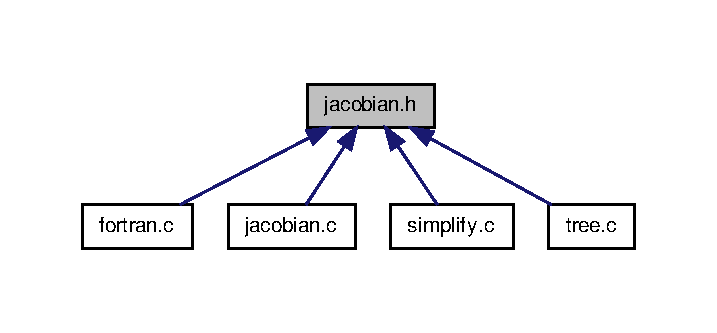
\includegraphics[width=344pt]{jacobian_8h__dep__incl}
\end{center}
\end{figure}
\subsection*{Functions}
\begin{DoxyCompactItemize}
\item 
void \hyperlink{jacobian_8h_a63b2497734bd2aea0c2648ee592913ae}{function\-To\-Jacobian} (struct \hyperlink{structNode}{Node} $\ast$t)
\item 
struct \hyperlink{structNode}{Node} $\ast$ \hyperlink{jacobian_8h_a679e6863209bf428a60f209b8ac64b2f}{derivative} (struct \hyperlink{structNode}{Node} $\ast$n, struct \hyperlink{structNode}{Node} $\ast$j)
\item 
char $\ast$ \hyperlink{jacobian_8h_a21d0cae9ba0f71cac6989332790340a4}{D} (char $\ast$name)
\item 
struct \hyperlink{structNode}{Node} $\ast$ \hyperlink{jacobian_8h_a7709640e1a5d9fdbe4b02d07e1389848}{D\-\_\-plus} (struct \hyperlink{structNode}{Node} $\ast$n1, struct \hyperlink{structNode}{Node} $\ast$n2, struct \hyperlink{structNode}{Node} $\ast$j)
\item 
struct \hyperlink{structNode}{Node} $\ast$ \hyperlink{jacobian_8h_a18e1538e30dfe1e4d675c9ae7e090912}{D\-\_\-minus} (struct \hyperlink{structNode}{Node} $\ast$n1, struct \hyperlink{structNode}{Node} $\ast$n2, struct \hyperlink{structNode}{Node} $\ast$j)
\item 
struct \hyperlink{structNode}{Node} $\ast$ \hyperlink{jacobian_8h_aabf319e76dcbd7f0f8135daea08130fb}{D\-\_\-negative} (struct \hyperlink{structNode}{Node} $\ast$n1, struct \hyperlink{structNode}{Node} $\ast$j)
\item 
struct \hyperlink{structNode}{Node} $\ast$ \hyperlink{jacobian_8h_a563b2d2ddf25802728e25a796247e051}{D\-\_\-mul} (struct \hyperlink{structNode}{Node} $\ast$n1, struct \hyperlink{structNode}{Node} $\ast$n2, struct \hyperlink{structNode}{Node} $\ast$j)
\item 
struct \hyperlink{structNode}{Node} $\ast$ \hyperlink{jacobian_8h_a7a5c37c4ee6200ad5b2ed80f44594f7d}{D\-\_\-div} (struct \hyperlink{structNode}{Node} $\ast$n1, struct \hyperlink{structNode}{Node} $\ast$n2, struct \hyperlink{structNode}{Node} $\ast$j)
\item 
struct \hyperlink{structNode}{Node} $\ast$ \hyperlink{jacobian_8h_ac69adbac2f1488631e322c8541d15c74}{D\-\_\-pow} (struct \hyperlink{structNode}{Node} $\ast$n1, struct \hyperlink{structNode}{Node} $\ast$n2, struct \hyperlink{structNode}{Node} $\ast$j)
\item 
struct \hyperlink{structNode}{Node} $\ast$ \hyperlink{jacobian_8h_adcb98e7d3dc6a9f4a69b2444a02ffc51}{D\-\_\-var} (struct \hyperlink{structNode}{Node} $\ast$n)
\item 
struct \hyperlink{structNode}{Node} $\ast$ \hyperlink{jacobian_8h_af7f82a4a6c2a7751ae8b1ddfeda4c7e7}{D\-\_\-assign} (struct \hyperlink{structNode}{Node} $\ast$n1, struct \hyperlink{structNode}{Node} $\ast$n2)
\item 
struct \hyperlink{structNode}{Node} $\ast$ \hyperlink{jacobian_8h_a39e38e4c1369d762f09f15c5e4e727a1}{D\-\_\-if} (struct \hyperlink{structNode}{Node} $\ast$n1, struct \hyperlink{structNode}{Node} $\ast$n2, struct \hyperlink{structNode}{Node} $\ast$j)
\item 
struct \hyperlink{structNode}{Node} $\ast$ \hyperlink{jacobian_8h_a66841a427a1ef221a92813ab9980933c}{D\-\_\-ifelse} (struct \hyperlink{structNode}{Node} $\ast$n1, struct \hyperlink{structNode}{Node} $\ast$n2, struct \hyperlink{structNode}{Node} $\ast$n3, struct \hyperlink{structNode}{Node} $\ast$j)
\item 
struct \hyperlink{structNode}{Node} $\ast$ \hyperlink{jacobian_8h_aa5e579b47c173b8044d76eaefe0f0ecf}{D\-\_\-for} (char $\ast$iden, struct \hyperlink{structNode}{Node} $\ast$n1, struct \hyperlink{structNode}{Node} $\ast$n2)
\item 
struct \hyperlink{structNode}{Node} $\ast$ \hyperlink{jacobian_8h_a9a73fec39d6f63181e0718e5af7a4580}{D\-\_\-zeros} (char $\ast$iden, struct \hyperlink{structNode}{Node} $\ast$n)
\item 
struct \hyperlink{structNode}{Node} $\ast$ \hyperlink{jacobian_8h_a5d2292d7cc66b8ab6bf756608e0e2b7a}{D\-\_\-arrayindex} (char $\ast$iden, struct \hyperlink{structNode}{Node} $\ast$n)
\item 
int \hyperlink{jacobian_8h_a840291bc02cba5474a4cb46a9b9566fe}{main} (void)
\end{DoxyCompactItemize}


\subsection{Function Documentation}
\hypertarget{jacobian_8h_a21d0cae9ba0f71cac6989332790340a4}{\index{jacobian.\-h@{jacobian.\-h}!D@{D}}
\index{D@{D}!jacobian.h@{jacobian.\-h}}
\subsubsection[{D}]{\setlength{\rightskip}{0pt plus 5cm}char$\ast$ D (
\begin{DoxyParamCaption}
\item[{char $\ast$}]{name}
\end{DoxyParamCaption}
)}}\label{jacobian_8h_a21d0cae9ba0f71cac6989332790340a4}
\hypertarget{jacobian_8h_a5d2292d7cc66b8ab6bf756608e0e2b7a}{\index{jacobian.\-h@{jacobian.\-h}!D\-\_\-arrayindex@{D\-\_\-arrayindex}}
\index{D\-\_\-arrayindex@{D\-\_\-arrayindex}!jacobian.h@{jacobian.\-h}}
\subsubsection[{D\-\_\-arrayindex}]{\setlength{\rightskip}{0pt plus 5cm}struct {\bf Node}$\ast$ D\-\_\-arrayindex (
\begin{DoxyParamCaption}
\item[{char $\ast$}]{iden, }
\item[{struct {\bf Node} $\ast$}]{n}
\end{DoxyParamCaption}
)}}\label{jacobian_8h_a5d2292d7cc66b8ab6bf756608e0e2b7a}
\hypertarget{jacobian_8h_af7f82a4a6c2a7751ae8b1ddfeda4c7e7}{\index{jacobian.\-h@{jacobian.\-h}!D\-\_\-assign@{D\-\_\-assign}}
\index{D\-\_\-assign@{D\-\_\-assign}!jacobian.h@{jacobian.\-h}}
\subsubsection[{D\-\_\-assign}]{\setlength{\rightskip}{0pt plus 5cm}struct {\bf Node}$\ast$ D\-\_\-assign (
\begin{DoxyParamCaption}
\item[{struct {\bf Node} $\ast$}]{n1, }
\item[{struct {\bf Node} $\ast$}]{n2}
\end{DoxyParamCaption}
)}}\label{jacobian_8h_af7f82a4a6c2a7751ae8b1ddfeda4c7e7}
\hypertarget{jacobian_8h_a7a5c37c4ee6200ad5b2ed80f44594f7d}{\index{jacobian.\-h@{jacobian.\-h}!D\-\_\-div@{D\-\_\-div}}
\index{D\-\_\-div@{D\-\_\-div}!jacobian.h@{jacobian.\-h}}
\subsubsection[{D\-\_\-div}]{\setlength{\rightskip}{0pt plus 5cm}struct {\bf Node}$\ast$ D\-\_\-div (
\begin{DoxyParamCaption}
\item[{struct {\bf Node} $\ast$}]{n1, }
\item[{struct {\bf Node} $\ast$}]{n2, }
\item[{struct {\bf Node} $\ast$}]{j}
\end{DoxyParamCaption}
)}}\label{jacobian_8h_a7a5c37c4ee6200ad5b2ed80f44594f7d}
\hypertarget{jacobian_8h_aa5e579b47c173b8044d76eaefe0f0ecf}{\index{jacobian.\-h@{jacobian.\-h}!D\-\_\-for@{D\-\_\-for}}
\index{D\-\_\-for@{D\-\_\-for}!jacobian.h@{jacobian.\-h}}
\subsubsection[{D\-\_\-for}]{\setlength{\rightskip}{0pt plus 5cm}struct {\bf Node}$\ast$ D\-\_\-for (
\begin{DoxyParamCaption}
\item[{char $\ast$}]{iden, }
\item[{struct {\bf Node} $\ast$}]{n1, }
\item[{struct {\bf Node} $\ast$}]{n2}
\end{DoxyParamCaption}
)}}\label{jacobian_8h_aa5e579b47c173b8044d76eaefe0f0ecf}
\hypertarget{jacobian_8h_a39e38e4c1369d762f09f15c5e4e727a1}{\index{jacobian.\-h@{jacobian.\-h}!D\-\_\-if@{D\-\_\-if}}
\index{D\-\_\-if@{D\-\_\-if}!jacobian.h@{jacobian.\-h}}
\subsubsection[{D\-\_\-if}]{\setlength{\rightskip}{0pt plus 5cm}struct {\bf Node}$\ast$ D\-\_\-if (
\begin{DoxyParamCaption}
\item[{struct {\bf Node} $\ast$}]{n1, }
\item[{struct {\bf Node} $\ast$}]{n2, }
\item[{struct {\bf Node} $\ast$}]{j}
\end{DoxyParamCaption}
)}}\label{jacobian_8h_a39e38e4c1369d762f09f15c5e4e727a1}
\hypertarget{jacobian_8h_a66841a427a1ef221a92813ab9980933c}{\index{jacobian.\-h@{jacobian.\-h}!D\-\_\-ifelse@{D\-\_\-ifelse}}
\index{D\-\_\-ifelse@{D\-\_\-ifelse}!jacobian.h@{jacobian.\-h}}
\subsubsection[{D\-\_\-ifelse}]{\setlength{\rightskip}{0pt plus 5cm}struct {\bf Node}$\ast$ D\-\_\-ifelse (
\begin{DoxyParamCaption}
\item[{struct {\bf Node} $\ast$}]{n1, }
\item[{struct {\bf Node} $\ast$}]{n2, }
\item[{struct {\bf Node} $\ast$}]{n3, }
\item[{struct {\bf Node} $\ast$}]{j}
\end{DoxyParamCaption}
)}}\label{jacobian_8h_a66841a427a1ef221a92813ab9980933c}
\hypertarget{jacobian_8h_a18e1538e30dfe1e4d675c9ae7e090912}{\index{jacobian.\-h@{jacobian.\-h}!D\-\_\-minus@{D\-\_\-minus}}
\index{D\-\_\-minus@{D\-\_\-minus}!jacobian.h@{jacobian.\-h}}
\subsubsection[{D\-\_\-minus}]{\setlength{\rightskip}{0pt plus 5cm}struct {\bf Node}$\ast$ D\-\_\-minus (
\begin{DoxyParamCaption}
\item[{struct {\bf Node} $\ast$}]{n1, }
\item[{struct {\bf Node} $\ast$}]{n2, }
\item[{struct {\bf Node} $\ast$}]{j}
\end{DoxyParamCaption}
)}}\label{jacobian_8h_a18e1538e30dfe1e4d675c9ae7e090912}
\hypertarget{jacobian_8h_a563b2d2ddf25802728e25a796247e051}{\index{jacobian.\-h@{jacobian.\-h}!D\-\_\-mul@{D\-\_\-mul}}
\index{D\-\_\-mul@{D\-\_\-mul}!jacobian.h@{jacobian.\-h}}
\subsubsection[{D\-\_\-mul}]{\setlength{\rightskip}{0pt plus 5cm}struct {\bf Node}$\ast$ D\-\_\-mul (
\begin{DoxyParamCaption}
\item[{struct {\bf Node} $\ast$}]{n1, }
\item[{struct {\bf Node} $\ast$}]{n2, }
\item[{struct {\bf Node} $\ast$}]{j}
\end{DoxyParamCaption}
)}}\label{jacobian_8h_a563b2d2ddf25802728e25a796247e051}
\hypertarget{jacobian_8h_aabf319e76dcbd7f0f8135daea08130fb}{\index{jacobian.\-h@{jacobian.\-h}!D\-\_\-negative@{D\-\_\-negative}}
\index{D\-\_\-negative@{D\-\_\-negative}!jacobian.h@{jacobian.\-h}}
\subsubsection[{D\-\_\-negative}]{\setlength{\rightskip}{0pt plus 5cm}struct {\bf Node}$\ast$ D\-\_\-negative (
\begin{DoxyParamCaption}
\item[{struct {\bf Node} $\ast$}]{n1, }
\item[{struct {\bf Node} $\ast$}]{j}
\end{DoxyParamCaption}
)}}\label{jacobian_8h_aabf319e76dcbd7f0f8135daea08130fb}
\hypertarget{jacobian_8h_a7709640e1a5d9fdbe4b02d07e1389848}{\index{jacobian.\-h@{jacobian.\-h}!D\-\_\-plus@{D\-\_\-plus}}
\index{D\-\_\-plus@{D\-\_\-plus}!jacobian.h@{jacobian.\-h}}
\subsubsection[{D\-\_\-plus}]{\setlength{\rightskip}{0pt plus 5cm}struct {\bf Node}$\ast$ D\-\_\-plus (
\begin{DoxyParamCaption}
\item[{struct {\bf Node} $\ast$}]{n1, }
\item[{struct {\bf Node} $\ast$}]{n2, }
\item[{struct {\bf Node} $\ast$}]{j}
\end{DoxyParamCaption}
)}}\label{jacobian_8h_a7709640e1a5d9fdbe4b02d07e1389848}
\hypertarget{jacobian_8h_ac69adbac2f1488631e322c8541d15c74}{\index{jacobian.\-h@{jacobian.\-h}!D\-\_\-pow@{D\-\_\-pow}}
\index{D\-\_\-pow@{D\-\_\-pow}!jacobian.h@{jacobian.\-h}}
\subsubsection[{D\-\_\-pow}]{\setlength{\rightskip}{0pt plus 5cm}struct {\bf Node}$\ast$ D\-\_\-pow (
\begin{DoxyParamCaption}
\item[{struct {\bf Node} $\ast$}]{n1, }
\item[{struct {\bf Node} $\ast$}]{n2, }
\item[{struct {\bf Node} $\ast$}]{j}
\end{DoxyParamCaption}
)}}\label{jacobian_8h_ac69adbac2f1488631e322c8541d15c74}
\hypertarget{jacobian_8h_adcb98e7d3dc6a9f4a69b2444a02ffc51}{\index{jacobian.\-h@{jacobian.\-h}!D\-\_\-var@{D\-\_\-var}}
\index{D\-\_\-var@{D\-\_\-var}!jacobian.h@{jacobian.\-h}}
\subsubsection[{D\-\_\-var}]{\setlength{\rightskip}{0pt plus 5cm}struct {\bf Node}$\ast$ D\-\_\-var (
\begin{DoxyParamCaption}
\item[{struct {\bf Node} $\ast$}]{n}
\end{DoxyParamCaption}
)}}\label{jacobian_8h_adcb98e7d3dc6a9f4a69b2444a02ffc51}
\hypertarget{jacobian_8h_a9a73fec39d6f63181e0718e5af7a4580}{\index{jacobian.\-h@{jacobian.\-h}!D\-\_\-zeros@{D\-\_\-zeros}}
\index{D\-\_\-zeros@{D\-\_\-zeros}!jacobian.h@{jacobian.\-h}}
\subsubsection[{D\-\_\-zeros}]{\setlength{\rightskip}{0pt plus 5cm}struct {\bf Node}$\ast$ D\-\_\-zeros (
\begin{DoxyParamCaption}
\item[{char $\ast$}]{iden, }
\item[{struct {\bf Node} $\ast$}]{n}
\end{DoxyParamCaption}
)}}\label{jacobian_8h_a9a73fec39d6f63181e0718e5af7a4580}
\hypertarget{jacobian_8h_a679e6863209bf428a60f209b8ac64b2f}{\index{jacobian.\-h@{jacobian.\-h}!derivative@{derivative}}
\index{derivative@{derivative}!jacobian.h@{jacobian.\-h}}
\subsubsection[{derivative}]{\setlength{\rightskip}{0pt plus 5cm}struct {\bf Node}$\ast$ derivative (
\begin{DoxyParamCaption}
\item[{struct {\bf Node} $\ast$}]{n, }
\item[{struct {\bf Node} $\ast$}]{j}
\end{DoxyParamCaption}
)}}\label{jacobian_8h_a679e6863209bf428a60f209b8ac64b2f}
\hypertarget{jacobian_8h_a63b2497734bd2aea0c2648ee592913ae}{\index{jacobian.\-h@{jacobian.\-h}!function\-To\-Jacobian@{function\-To\-Jacobian}}
\index{function\-To\-Jacobian@{function\-To\-Jacobian}!jacobian.h@{jacobian.\-h}}
\subsubsection[{function\-To\-Jacobian}]{\setlength{\rightskip}{0pt plus 5cm}void function\-To\-Jacobian (
\begin{DoxyParamCaption}
\item[{struct {\bf Node} $\ast$}]{t}
\end{DoxyParamCaption}
)}}\label{jacobian_8h_a63b2497734bd2aea0c2648ee592913ae}
\hypertarget{jacobian_8h_a840291bc02cba5474a4cb46a9b9566fe}{\index{jacobian.\-h@{jacobian.\-h}!main@{main}}
\index{main@{main}!jacobian.h@{jacobian.\-h}}
\subsubsection[{main}]{\setlength{\rightskip}{0pt plus 5cm}int main (
\begin{DoxyParamCaption}
\item[{void}]{}
\end{DoxyParamCaption}
)}}\label{jacobian_8h_a840291bc02cba5474a4cb46a9b9566fe}

\hypertarget{node_8c}{\section{node.\-c File Reference}
\label{node_8c}\index{node.\-c@{node.\-c}}
}
{\ttfamily \#include $<$stdio.\-h$>$}\\*
{\ttfamily \#include $<$stdlib.\-h$>$}\\*
{\ttfamily \#include $<$string.\-h$>$}\\*
{\ttfamily \#include \char`\"{}node.\-h\char`\"{}}\\*
{\ttfamily \#include \char`\"{}tree.\-h\char`\"{}}\\*
Include dependency graph for node.\-c\-:\nopagebreak
\begin{figure}[H]
\begin{center}
\leavevmode
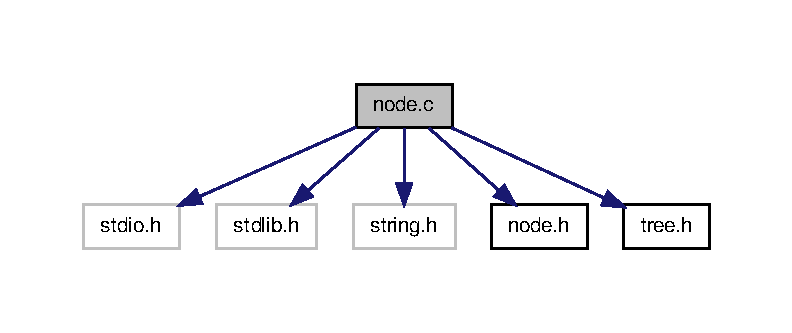
\includegraphics[width=350pt]{node_8c__incl}
\end{center}
\end{figure}
\subsection*{Functions}
\begin{DoxyCompactItemize}
\item 
struct \hyperlink{structNode}{Node} $\ast$ \hyperlink{node_8c_a8021c7e05df0eb5a301433b6a83a5751}{last} (struct \hyperlink{structNode}{Node} $\ast$t)
\begin{DoxyCompactList}\small\item\em Find the last \hyperlink{structNode}{Node} on the same level as the specified \hyperlink{structNode}{Node}. \end{DoxyCompactList}\item 
struct \hyperlink{structNode}{Node} $\ast$ \hyperlink{node_8c_a990974952aa48d789ee7dabf10070194}{create\-Operation} (enum \hyperlink{node_8h_a83ba1e84fa23f6619c3d29036b160919}{Node\-Tag} op)
\begin{DoxyCompactList}\small\item\em Create a \hyperlink{structNode}{Node} of the specified operation type. \end{DoxyCompactList}\item 
void \hyperlink{node_8c_ac59e12e2146890bd3656810716854c5f}{append\-Child} (struct \hyperlink{structNode}{Node} $\ast$parent, struct \hyperlink{structNode}{Node} $\ast$child)
\begin{DoxyCompactList}\small\item\em Append a child \hyperlink{structNode}{Node} to a parent \hyperlink{structNode}{Node}. \end{DoxyCompactList}\item 
void \hyperlink{node_8c_ad1f8d800997fdede9718ede6b9b2d741}{set\-Identifier} (struct \hyperlink{structNode}{Node} $\ast$node, char $\ast$identifier)
\begin{DoxyCompactList}\small\item\em Set the identifier of a \hyperlink{structNode}{Node}. \end{DoxyCompactList}\item 
struct \hyperlink{structNode}{Node} $\ast$ \hyperlink{node_8c_aa603e9647cbbe4208a6de5546df7b9f7}{create\-Constant} (double num)
\begin{DoxyCompactList}\small\item\em Create a \hyperlink{structNode}{Node} representing a constant number. \end{DoxyCompactList}\item 
struct \hyperlink{structNode}{Node} $\ast$ \hyperlink{node_8c_a25b6be3754d0bfe7f721c65986872f75}{create\-Variable} (char $\ast$varname)
\begin{DoxyCompactList}\small\item\em Create a \hyperlink{structNode}{Node} representing a variable. \end{DoxyCompactList}\item 
struct \hyperlink{structNode}{Node} $\ast$ \hyperlink{node_8c_a36f4e62840cea8119a80005c7093c1a2}{append\-Statement} (struct \hyperlink{structNode}{Node} $\ast$prevnodes, struct \hyperlink{structNode}{Node} $\ast$newnode)
\begin{DoxyCompactList}\small\item\em Append a statement to a list of statements. \end{DoxyCompactList}\item 
struct \hyperlink{structNode}{Node} $\ast$ \hyperlink{node_8c_a630e9a32f8dad634171441534eedd274}{copy\-Node} (struct \hyperlink{structNode}{Node} $\ast$n)
\begin{DoxyCompactList}\small\item\em Copies the data of a \hyperlink{structNode}{Node} to a new \hyperlink{structNode}{Node} instance. \end{DoxyCompactList}\item 
struct \hyperlink{structNode}{Node} $\ast$ \hyperlink{node_8c_ab62128f06e9ecf1ba999035e44e20125}{find\-Variable} (struct \hyperlink{structNode}{Node} $\ast$n)
\item 
int \hyperlink{node_8c_af424017909286f07f58ff8bcc1cb16ca}{compare\-Nodes} (struct \hyperlink{structNode}{Node} $\ast$n1, struct \hyperlink{structNode}{Node} $\ast$n2)
\begin{DoxyCompactList}\small\item\em Compare two Nodes and their children to check whether they are equivalent. \end{DoxyCompactList}\item 
void \hyperlink{node_8c_a9404ea17c515d0d18c37bde7c31b5979}{remove\-Node} (struct \hyperlink{structNode}{Node} $\ast$n)
\begin{DoxyCompactList}\small\item\em Remove an \hyperlink{structNode}{Node} instance and free the memory it used. \end{DoxyCompactList}\end{DoxyCompactItemize}


\subsection{Function Documentation}
\hypertarget{node_8c_ac59e12e2146890bd3656810716854c5f}{\index{node.\-c@{node.\-c}!append\-Child@{append\-Child}}
\index{append\-Child@{append\-Child}!node.c@{node.\-c}}
\subsubsection[{append\-Child}]{\setlength{\rightskip}{0pt plus 5cm}void append\-Child (
\begin{DoxyParamCaption}
\item[{struct {\bf Node} $\ast$}]{parent, }
\item[{struct {\bf Node} $\ast$}]{child}
\end{DoxyParamCaption}
)}}\label{node_8c_ac59e12e2146890bd3656810716854c5f}


Append a child \hyperlink{structNode}{Node} to a parent \hyperlink{structNode}{Node}. 

Append the \hyperlink{structNode}{Node} {\itshape child} to the list of children of \hyperlink{structNode}{Node} {\itshape parent} and sets {\itshape parent} as the parent \hyperlink{structNode}{Node} of {\itshape child}. 
\begin{DoxyParams}{Parameters}
{\em parent} & \hyperlink{structNode}{Node} where the {\itshape child} \hyperlink{structNode}{Node} is to be appended to. \\
\hline
{\em child} & \hyperlink{structNode}{Node} to be appended to the children of {\itshape parent}. \\
\hline
\end{DoxyParams}
\hypertarget{node_8c_a36f4e62840cea8119a80005c7093c1a2}{\index{node.\-c@{node.\-c}!append\-Statement@{append\-Statement}}
\index{append\-Statement@{append\-Statement}!node.c@{node.\-c}}
\subsubsection[{append\-Statement}]{\setlength{\rightskip}{0pt plus 5cm}struct {\bf Node}$\ast$ append\-Statement (
\begin{DoxyParamCaption}
\item[{struct {\bf Node} $\ast$}]{prevnodes, }
\item[{struct {\bf Node} $\ast$}]{newnode}
\end{DoxyParamCaption}
)}}\label{node_8c_a36f4e62840cea8119a80005c7093c1a2}


Append a statement to a list of statements. 

Appends the statement {\itshape newnode} to the list of statements {\itshape prevnodes}. {\itshape prevnodes} does not have to point at the last \hyperlink{structNode}{Node} of that level. This function will find the last \hyperlink{structNode}{Node} of the same level and append the {\itshape newnode} there. 
\begin{DoxyParams}{Parameters}
{\em prevnodes} & Pointer to a \hyperlink{structNode}{Node} on which level the \hyperlink{structNode}{Node} {\itshape newnode} should be added. \\
\hline
{\em newnode} & \hyperlink{structNode}{Node} to add to the linked list. \\
\hline
\end{DoxyParams}
\begin{DoxyReturn}{Returns}
Pointer to a \hyperlink{structNode}{Node} of the level where {\itshape newnode} was added. 
\end{DoxyReturn}
\hypertarget{node_8c_af424017909286f07f58ff8bcc1cb16ca}{\index{node.\-c@{node.\-c}!compare\-Nodes@{compare\-Nodes}}
\index{compare\-Nodes@{compare\-Nodes}!node.c@{node.\-c}}
\subsubsection[{compare\-Nodes}]{\setlength{\rightskip}{0pt plus 5cm}int compare\-Nodes (
\begin{DoxyParamCaption}
\item[{struct {\bf Node} $\ast$}]{n1, }
\item[{struct {\bf Node} $\ast$}]{n2}
\end{DoxyParamCaption}
)}}\label{node_8c_af424017909286f07f58ff8bcc1cb16ca}


Compare two Nodes and their children to check whether they are equivalent. 

Compare the Nodes {\itshape n1} and {\itshape n2} and their children to check whether they are equivalent. All properties of the \hyperlink{structNode}{Node} struct are compared, just like the complete structure the Nodes represent. 
\begin{DoxyParams}{Parameters}
{\em n1} & First \hyperlink{structNode}{Node}. \\
\hline
{\em n2} & Second \hyperlink{structNode}{Node}. \\
\hline
\end{DoxyParams}
\begin{DoxyReturn}{Returns}
1 when the first and second \hyperlink{structNode}{Node} are equivalent, 0 otherwise. 
\end{DoxyReturn}
\hypertarget{node_8c_a630e9a32f8dad634171441534eedd274}{\index{node.\-c@{node.\-c}!copy\-Node@{copy\-Node}}
\index{copy\-Node@{copy\-Node}!node.c@{node.\-c}}
\subsubsection[{copy\-Node}]{\setlength{\rightskip}{0pt plus 5cm}struct {\bf Node}$\ast$ copy\-Node (
\begin{DoxyParamCaption}
\item[{struct {\bf Node} $\ast$}]{n}
\end{DoxyParamCaption}
)}}\label{node_8c_a630e9a32f8dad634171441534eedd274}


Copies the data of a \hyperlink{structNode}{Node} to a new \hyperlink{structNode}{Node} instance. 

Copy the contents of \hyperlink{structNode}{Node} {\itshape n} to a new \hyperlink{structNode}{Node} and recursively does the same to all children. The neighbours of \hyperlink{structNode}{Node} {\itshape n} will not be copied. 
\begin{DoxyParams}{Parameters}
{\em n} & \hyperlink{structNode}{Node} to copy. \\
\hline
\end{DoxyParams}
\begin{DoxyReturn}{Returns}
Pointer to the new \hyperlink{structNode}{Node} with the same data as {\itshape n}. 
\end{DoxyReturn}
\hypertarget{node_8c_aa603e9647cbbe4208a6de5546df7b9f7}{\index{node.\-c@{node.\-c}!create\-Constant@{create\-Constant}}
\index{create\-Constant@{create\-Constant}!node.c@{node.\-c}}
\subsubsection[{create\-Constant}]{\setlength{\rightskip}{0pt plus 5cm}struct {\bf Node}$\ast$ create\-Constant (
\begin{DoxyParamCaption}
\item[{double}]{num}
\end{DoxyParamCaption}
)}}\label{node_8c_aa603e9647cbbe4208a6de5546df7b9f7}


Create a \hyperlink{structNode}{Node} representing a constant number. 

Create a \hyperlink{structNode}{Node} representing the number {\itshape num}. 
\begin{DoxyParams}{Parameters}
{\em num} & The value of the constant. \\
\hline
\end{DoxyParams}
\begin{DoxyReturn}{Returns}
Pointer to the created \hyperlink{structNode}{Node} instance. 
\end{DoxyReturn}
\hypertarget{node_8c_a990974952aa48d789ee7dabf10070194}{\index{node.\-c@{node.\-c}!create\-Operation@{create\-Operation}}
\index{create\-Operation@{create\-Operation}!node.c@{node.\-c}}
\subsubsection[{create\-Operation}]{\setlength{\rightskip}{0pt plus 5cm}struct {\bf Node}$\ast$ create\-Operation (
\begin{DoxyParamCaption}
\item[{enum {\bf Node\-Tag}}]{op}
\end{DoxyParamCaption}
)}}\label{node_8c_a990974952aa48d789ee7dabf10070194}


Create a \hyperlink{structNode}{Node} of the specified operation type. 

Create a \hyperlink{structNode}{Node} of the specified operation, whilst setting all other properties to zero or N\-U\-L\-L. 
\begin{DoxyParams}{Parameters}
{\em op} & Operation type of the \hyperlink{structNode}{Node} to be created. \\
\hline
\end{DoxyParams}
\begin{DoxyReturn}{Returns}
The created \hyperlink{structNode}{Node} instance. 
\end{DoxyReturn}
\hypertarget{node_8c_a25b6be3754d0bfe7f721c65986872f75}{\index{node.\-c@{node.\-c}!create\-Variable@{create\-Variable}}
\index{create\-Variable@{create\-Variable}!node.c@{node.\-c}}
\subsubsection[{create\-Variable}]{\setlength{\rightskip}{0pt plus 5cm}struct {\bf Node}$\ast$ create\-Variable (
\begin{DoxyParamCaption}
\item[{char $\ast$}]{varname}
\end{DoxyParamCaption}
)}}\label{node_8c_a25b6be3754d0bfe7f721c65986872f75}


Create a \hyperlink{structNode}{Node} representing a variable. 

Create a \hyperlink{structNode}{Node} representing a variable with the name {\itshape varname}. 
\begin{DoxyParams}{Parameters}
{\em varname} & The name of the variable. \\
\hline
\end{DoxyParams}
\begin{DoxyReturn}{Returns}
Pointer to the created \hyperlink{structNode}{Node} instance. 
\end{DoxyReturn}
\hypertarget{node_8c_ab62128f06e9ecf1ba999035e44e20125}{\index{node.\-c@{node.\-c}!find\-Variable@{find\-Variable}}
\index{find\-Variable@{find\-Variable}!node.c@{node.\-c}}
\subsubsection[{find\-Variable}]{\setlength{\rightskip}{0pt plus 5cm}struct {\bf Node}$\ast$ find\-Variable (
\begin{DoxyParamCaption}
\item[{struct {\bf Node} $\ast$}]{n}
\end{DoxyParamCaption}
)}}\label{node_8c_ab62128f06e9ecf1ba999035e44e20125}
\begin{DoxyRefDesc}{Todo}
\item[\hyperlink{todo__todo000001}{Todo}]Describe this function \end{DoxyRefDesc}
\hypertarget{node_8c_a8021c7e05df0eb5a301433b6a83a5751}{\index{node.\-c@{node.\-c}!last@{last}}
\index{last@{last}!node.c@{node.\-c}}
\subsubsection[{last}]{\setlength{\rightskip}{0pt plus 5cm}struct {\bf Node}$\ast$ last (
\begin{DoxyParamCaption}
\item[{struct {\bf Node} $\ast$}]{t}
\end{DoxyParamCaption}
)}}\label{node_8c_a8021c7e05df0eb5a301433b6a83a5751}


Find the last \hyperlink{structNode}{Node} on the same level as the specified \hyperlink{structNode}{Node}. 

Search the last \hyperlink{structNode}{Node} on the same level as \hyperlink{structNode}{Node} {\itshape t}. 
\begin{DoxyParams}{Parameters}
{\em t} & \hyperlink{structNode}{Node} of which to find the last neighbour/peer. \\
\hline
\end{DoxyParams}
\begin{DoxyReturn}{Returns}
The last \hyperlink{structNode}{Node} on the same level as \hyperlink{structNode}{Node} {\itshape t}. 
\end{DoxyReturn}
\hypertarget{node_8c_a9404ea17c515d0d18c37bde7c31b5979}{\index{node.\-c@{node.\-c}!remove\-Node@{remove\-Node}}
\index{remove\-Node@{remove\-Node}!node.c@{node.\-c}}
\subsubsection[{remove\-Node}]{\setlength{\rightskip}{0pt plus 5cm}void remove\-Node (
\begin{DoxyParamCaption}
\item[{struct {\bf Node} $\ast$}]{n}
\end{DoxyParamCaption}
)}}\label{node_8c_a9404ea17c515d0d18c37bde7c31b5979}


Remove an \hyperlink{structNode}{Node} instance and free the memory it used. 

Removes \hyperlink{structNode}{Node} {\itshape n} and all its children. 
\begin{DoxyParams}{Parameters}
{\em n} & \hyperlink{structNode}{Node} to remove. \\
\hline
\end{DoxyParams}
\hypertarget{node_8c_ad1f8d800997fdede9718ede6b9b2d741}{\index{node.\-c@{node.\-c}!set\-Identifier@{set\-Identifier}}
\index{set\-Identifier@{set\-Identifier}!node.c@{node.\-c}}
\subsubsection[{set\-Identifier}]{\setlength{\rightskip}{0pt plus 5cm}void set\-Identifier (
\begin{DoxyParamCaption}
\item[{struct {\bf Node} $\ast$}]{node, }
\item[{char $\ast$}]{identifier}
\end{DoxyParamCaption}
)}}\label{node_8c_ad1f8d800997fdede9718ede6b9b2d741}


Set the identifier of a \hyperlink{structNode}{Node}. 

Set the identifier (\hyperlink{structNode_a76c70ae7ac3d58ebe41da968fedb8093}{Node\-::iname}) of \hyperlink{structNode}{Node} {\itshape node} to {\itshape identifier}. 
\begin{DoxyParams}{Parameters}
{\em node} & \hyperlink{structNode}{Node} to set the identifier of. \\
\hline
{\em identifier} & Name of the identifier. \\
\hline
\end{DoxyParams}

\hypertarget{node_8h}{\section{node.\-h File Reference}
\label{node_8h}\index{node.\-h@{node.\-h}}
}
This graph shows which files directly or indirectly include this file\-:\nopagebreak
\begin{figure}[H]
\begin{center}
\leavevmode
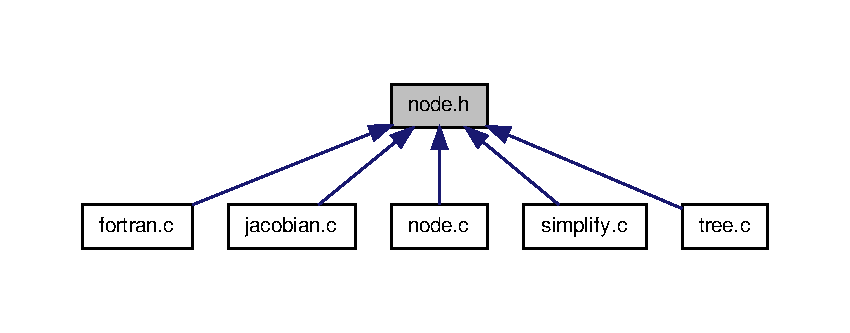
\includegraphics[width=350pt]{node_8h__dep__incl}
\end{center}
\end{figure}
\subsection*{Data Structures}
\begin{DoxyCompactItemize}
\item 
struct \hyperlink{structNode}{Node}
\begin{DoxyCompactList}\small\item\em A two dimensional node/tree data. \end{DoxyCompactList}\end{DoxyCompactItemize}
\subsection*{Enumerations}
\begin{DoxyCompactItemize}
\item 
enum \hyperlink{node_8h_a83ba1e84fa23f6619c3d29036b160919}{Node\-Tag} \{ \\*
\hyperlink{node_8h_a83ba1e84fa23f6619c3d29036b160919ab61d4391af9740a542e317b9ce6a3d2e}{T\-P\-L\-U\-S}, 
\hyperlink{node_8h_a83ba1e84fa23f6619c3d29036b160919a229e1fa5893725d4ab9141de9a5221c3}{T\-M\-I\-N\-U\-S}, 
\hyperlink{node_8h_a83ba1e84fa23f6619c3d29036b160919a2f6da8014bbb780265737f3edb98f928}{T\-M\-U\-L}, 
\hyperlink{node_8h_a83ba1e84fa23f6619c3d29036b160919ac3e4cf6bb26322af5dcabd9a3e536863}{T\-D\-I\-V}, 
\\*
\hyperlink{node_8h_a83ba1e84fa23f6619c3d29036b160919ac9f2843a55469a6152dd35687d275193}{T\-P\-O\-W}, 
\hyperlink{node_8h_a83ba1e84fa23f6619c3d29036b160919a71fff872f388505135681e9fad482e72}{T\-N\-U\-M}, 
\hyperlink{node_8h_a83ba1e84fa23f6619c3d29036b160919afe64957b6fe1c660804c3d310000b5f0}{T\-V\-A\-R}, 
\hyperlink{node_8h_a83ba1e84fa23f6619c3d29036b160919aae1cac6fabc93853164889cdc0d77b1a}{T\-F\-O\-R}, 
\\*
\hyperlink{node_8h_a83ba1e84fa23f6619c3d29036b160919aaf9a72d2b433486eb715922b4c98b19b}{T\-W\-H\-I\-L\-E}, 
\hyperlink{node_8h_a83ba1e84fa23f6619c3d29036b160919a8583540b6f599086fc9753a345cedba8}{T\-A\-S\-S\-I\-G\-N}, 
\hyperlink{node_8h_a83ba1e84fa23f6619c3d29036b160919a1ba33d59e4de7364510db374755b7d7e}{T\-R\-A\-N\-G\-E}, 
\hyperlink{node_8h_a83ba1e84fa23f6619c3d29036b160919ada27aaee300d100894b7052b2063d6dd}{T\-O\-R}, 
\\*
\hyperlink{node_8h_a83ba1e84fa23f6619c3d29036b160919ac83acf67a25689b50ade68bb2c59391f}{T\-A\-N\-D}, 
\hyperlink{node_8h_a83ba1e84fa23f6619c3d29036b160919a2628d0015da0ba3baca55ea90b6bdeba}{T\-E\-Q\-\_\-\-O\-P}, 
\hyperlink{node_8h_a83ba1e84fa23f6619c3d29036b160919ada7148d13131a5296980f6158b94f9b6}{T\-N\-E\-\_\-\-O\-P}, 
\hyperlink{node_8h_a83ba1e84fa23f6619c3d29036b160919a275466a9a49ca2f6b9aac4c714420bd0}{T\-G\-T\-\_\-\-O\-P}, 
\\*
\hyperlink{node_8h_a83ba1e84fa23f6619c3d29036b160919a69747867f677928f5b44b50be82e355a}{T\-L\-T\-\_\-\-O\-P}, 
\hyperlink{node_8h_a83ba1e84fa23f6619c3d29036b160919aa7765aa3b3c0d91d3bb14099258f72f3}{T\-G\-E\-\_\-\-O\-P}, 
\hyperlink{node_8h_a83ba1e84fa23f6619c3d29036b160919a06cb01dea3f4bfae79d87b0534c0a221}{T\-L\-E\-\_\-\-O\-P}, 
\hyperlink{node_8h_a83ba1e84fa23f6619c3d29036b160919af6049a2c76faf4a885590098b3c6f5d7}{T\-I\-F}, 
\\*
\hyperlink{node_8h_a83ba1e84fa23f6619c3d29036b160919a2f21ceca5171b4c27f561a3abdac8cd9}{T\-I\-F\-E\-L\-S\-E}, 
\hyperlink{node_8h_a83ba1e84fa23f6619c3d29036b160919a00caba3d6b9ef9fa9adeed58f0fab5ae}{T\-I\-F\-E\-L\-S\-E\-I\-F}, 
\hyperlink{node_8h_a83ba1e84fa23f6619c3d29036b160919a2c176bcae51056202bb3b10ca15bec6c}{T\-E\-L\-S\-E\-I\-F}, 
\hyperlink{node_8h_a83ba1e84fa23f6619c3d29036b160919a47618f8f65141735078edfa809d0e93c}{T\-I\-F\-E\-L\-S\-E\-I\-F\-E\-L\-S\-E}, 
\\*
\hyperlink{node_8h_a83ba1e84fa23f6619c3d29036b160919a5b179cf7f0b8747fa3f686c8d7cdc2aa}{T\-A\-R\-R\-A\-Y\-I\-N\-D\-E\-X}, 
\hyperlink{node_8h_a83ba1e84fa23f6619c3d29036b160919aeeb11e0d29bd5515538fc54998e73698}{T\-L\-I\-S\-T}, 
\hyperlink{node_8h_a83ba1e84fa23f6619c3d29036b160919a3b314fffc527699e89b8904804e41bfe}{T\-F\-U\-N\-C\-D\-E\-C}, 
\hyperlink{node_8h_a83ba1e84fa23f6619c3d29036b160919ac66d28545a7441c95c8ef80bb8c72ce2}{T\-M\-I\-S\-C}, 
\\*
\hyperlink{node_8h_a83ba1e84fa23f6619c3d29036b160919a8d8ec3ec1fab79e3ecb560657481efc9}{T\-C\-O\-M\-B\-I\-N\-E}, 
\hyperlink{node_8h_a83ba1e84fa23f6619c3d29036b160919aecc032ac8d73ded1632db71be06e61a9}{T\-N\-O\-T}, 
\hyperlink{node_8h_a83ba1e84fa23f6619c3d29036b160919adca0a7f9ec50a9d85eb8b1852387be0d}{T\-N\-E\-G\-A\-T\-I\-V\-E}
 \}
\begin{DoxyCompactList}\small\item\em Tags the \hyperlink{structNode}{Node} struct uses to specify its type or purpose. \end{DoxyCompactList}\end{DoxyCompactItemize}
\subsection*{Functions}
\begin{DoxyCompactItemize}
\item 
struct \hyperlink{structNode}{Node} $\ast$ \hyperlink{node_8h_a990974952aa48d789ee7dabf10070194}{create\-Operation} (enum \hyperlink{node_8h_a83ba1e84fa23f6619c3d29036b160919}{Node\-Tag} op)
\begin{DoxyCompactList}\small\item\em Create a \hyperlink{structNode}{Node} of the specified operation type. \end{DoxyCompactList}\item 
void \hyperlink{node_8h_ac59e12e2146890bd3656810716854c5f}{append\-Child} (struct \hyperlink{structNode}{Node} $\ast$parent, struct \hyperlink{structNode}{Node} $\ast$child)
\begin{DoxyCompactList}\small\item\em Append a child \hyperlink{structNode}{Node} to a parent \hyperlink{structNode}{Node}. \end{DoxyCompactList}\item 
void \hyperlink{node_8h_ad1f8d800997fdede9718ede6b9b2d741}{set\-Identifier} (struct \hyperlink{structNode}{Node} $\ast$node, char $\ast$identifier)
\begin{DoxyCompactList}\small\item\em Set the identifier of a \hyperlink{structNode}{Node}. \end{DoxyCompactList}\item 
struct \hyperlink{structNode}{Node} $\ast$ \hyperlink{node_8h_a8021c7e05df0eb5a301433b6a83a5751}{last} (struct \hyperlink{structNode}{Node} $\ast$t)
\begin{DoxyCompactList}\small\item\em Find the last \hyperlink{structNode}{Node} on the same level as the specified \hyperlink{structNode}{Node}. \end{DoxyCompactList}\item 
struct \hyperlink{structNode}{Node} $\ast$ \hyperlink{node_8h_aa603e9647cbbe4208a6de5546df7b9f7}{create\-Constant} (double num)
\begin{DoxyCompactList}\small\item\em Create a \hyperlink{structNode}{Node} representing a constant number. \end{DoxyCompactList}\item 
struct \hyperlink{structNode}{Node} $\ast$ \hyperlink{node_8h_a25b6be3754d0bfe7f721c65986872f75}{create\-Variable} (char $\ast$varname)
\begin{DoxyCompactList}\small\item\em Create a \hyperlink{structNode}{Node} representing a variable. \end{DoxyCompactList}\item 
struct \hyperlink{structNode}{Node} $\ast$ \hyperlink{node_8h_a36f4e62840cea8119a80005c7093c1a2}{append\-Statement} (struct \hyperlink{structNode}{Node} $\ast$prevnodes, struct \hyperlink{structNode}{Node} $\ast$newnode)
\begin{DoxyCompactList}\small\item\em Append a statement to a list of statements. \end{DoxyCompactList}\item 
struct \hyperlink{structNode}{Node} $\ast$ \hyperlink{node_8h_a630e9a32f8dad634171441534eedd274}{copy\-Node} (struct \hyperlink{structNode}{Node} $\ast$n)
\begin{DoxyCompactList}\small\item\em Copies the data of a \hyperlink{structNode}{Node} to a new \hyperlink{structNode}{Node} instance. \end{DoxyCompactList}\item 
void \hyperlink{node_8h_a9404ea17c515d0d18c37bde7c31b5979}{remove\-Node} (struct \hyperlink{structNode}{Node} $\ast$n)
\begin{DoxyCompactList}\small\item\em Remove an \hyperlink{structNode}{Node} instance and free the memory it used. \end{DoxyCompactList}\item 
struct \hyperlink{structNode}{Node} $\ast$ \hyperlink{node_8h_ab62128f06e9ecf1ba999035e44e20125}{find\-Variable} (struct \hyperlink{structNode}{Node} $\ast$n)
\item 
int \hyperlink{node_8h_af424017909286f07f58ff8bcc1cb16ca}{compare\-Nodes} (struct \hyperlink{structNode}{Node} $\ast$n1, struct \hyperlink{structNode}{Node} $\ast$n2)
\begin{DoxyCompactList}\small\item\em Compare two Nodes and their children to check whether they are equivalent. \end{DoxyCompactList}\end{DoxyCompactItemize}


\subsection{Enumeration Type Documentation}
\hypertarget{node_8h_a83ba1e84fa23f6619c3d29036b160919}{\index{node.\-h@{node.\-h}!Node\-Tag@{Node\-Tag}}
\index{Node\-Tag@{Node\-Tag}!node.h@{node.\-h}}
\subsubsection[{Node\-Tag}]{\setlength{\rightskip}{0pt plus 5cm}enum {\bf Node\-Tag}}}\label{node_8h_a83ba1e84fa23f6619c3d29036b160919}


Tags the \hyperlink{structNode}{Node} struct uses to specify its type or purpose. 

\begin{Desc}
\item[Enumerator]\par
\begin{description}
\index{T\-P\-L\-U\-S@{T\-P\-L\-U\-S}!node.\-h@{node.\-h}}\index{node.\-h@{node.\-h}!T\-P\-L\-U\-S@{T\-P\-L\-U\-S}}\item[{\em 
\hypertarget{node_8h_a83ba1e84fa23f6619c3d29036b160919ab61d4391af9740a542e317b9ce6a3d2e}{T\-P\-L\-U\-S}\label{node_8h_a83ba1e84fa23f6619c3d29036b160919ab61d4391af9740a542e317b9ce6a3d2e}
}]Plus operation (a+b), two children. \index{T\-M\-I\-N\-U\-S@{T\-M\-I\-N\-U\-S}!node.\-h@{node.\-h}}\index{node.\-h@{node.\-h}!T\-M\-I\-N\-U\-S@{T\-M\-I\-N\-U\-S}}\item[{\em 
\hypertarget{node_8h_a83ba1e84fa23f6619c3d29036b160919a229e1fa5893725d4ab9141de9a5221c3}{T\-M\-I\-N\-U\-S}\label{node_8h_a83ba1e84fa23f6619c3d29036b160919a229e1fa5893725d4ab9141de9a5221c3}
}]Minus operation (a-\/b), two children. \index{T\-M\-U\-L@{T\-M\-U\-L}!node.\-h@{node.\-h}}\index{node.\-h@{node.\-h}!T\-M\-U\-L@{T\-M\-U\-L}}\item[{\em 
\hypertarget{node_8h_a83ba1e84fa23f6619c3d29036b160919a2f6da8014bbb780265737f3edb98f928}{T\-M\-U\-L}\label{node_8h_a83ba1e84fa23f6619c3d29036b160919a2f6da8014bbb780265737f3edb98f928}
}]Multiplication operation (a$\ast$b), two children. \index{T\-D\-I\-V@{T\-D\-I\-V}!node.\-h@{node.\-h}}\index{node.\-h@{node.\-h}!T\-D\-I\-V@{T\-D\-I\-V}}\item[{\em 
\hypertarget{node_8h_a83ba1e84fa23f6619c3d29036b160919ac3e4cf6bb26322af5dcabd9a3e536863}{T\-D\-I\-V}\label{node_8h_a83ba1e84fa23f6619c3d29036b160919ac3e4cf6bb26322af5dcabd9a3e536863}
}]Division operation (a/b), two children. \index{T\-P\-O\-W@{T\-P\-O\-W}!node.\-h@{node.\-h}}\index{node.\-h@{node.\-h}!T\-P\-O\-W@{T\-P\-O\-W}}\item[{\em 
\hypertarget{node_8h_a83ba1e84fa23f6619c3d29036b160919ac9f2843a55469a6152dd35687d275193}{T\-P\-O\-W}\label{node_8h_a83ba1e84fa23f6619c3d29036b160919ac9f2843a55469a6152dd35687d275193}
}]Power operation (a$^\wedge$b; a$\ast$$\ast$b), two children. \index{T\-N\-U\-M@{T\-N\-U\-M}!node.\-h@{node.\-h}}\index{node.\-h@{node.\-h}!T\-N\-U\-M@{T\-N\-U\-M}}\item[{\em 
\hypertarget{node_8h_a83ba1e84fa23f6619c3d29036b160919a71fff872f388505135681e9fad482e72}{T\-N\-U\-M}\label{node_8h_a83ba1e84fa23f6619c3d29036b160919a71fff872f388505135681e9fad482e72}
}]Number, no children. \hyperlink{structNode_ad7f9455e819b623c0e4a9480476eacfe}{Node\-::ival} should be specified. \index{T\-V\-A\-R@{T\-V\-A\-R}!node.\-h@{node.\-h}}\index{node.\-h@{node.\-h}!T\-V\-A\-R@{T\-V\-A\-R}}\item[{\em 
\hypertarget{node_8h_a83ba1e84fa23f6619c3d29036b160919afe64957b6fe1c660804c3d310000b5f0}{T\-V\-A\-R}\label{node_8h_a83ba1e84fa23f6619c3d29036b160919afe64957b6fe1c660804c3d310000b5f0}
}]\hyperlink{structVariable}{Variable}, no children. \hyperlink{structNode_a76c70ae7ac3d58ebe41da968fedb8093}{Node\-::iname} should be specified. \index{T\-F\-O\-R@{T\-F\-O\-R}!node.\-h@{node.\-h}}\index{node.\-h@{node.\-h}!T\-F\-O\-R@{T\-F\-O\-R}}\item[{\em 
\hypertarget{node_8h_a83ba1e84fa23f6619c3d29036b160919aae1cac6fabc93853164889cdc0d77b1a}{T\-F\-O\-R}\label{node_8h_a83ba1e84fa23f6619c3d29036b160919aae1cac6fabc93853164889cdc0d77b1a}
}]For statement, at least 2 children. \hyperlink{structNode_a76c70ae7ac3d58ebe41da968fedb8093}{Node\-::iname} should be specified. The first child specifies a range, the subsequent statements are sub-\/statements of the for loop. \index{T\-W\-H\-I\-L\-E@{T\-W\-H\-I\-L\-E}!node.\-h@{node.\-h}}\index{node.\-h@{node.\-h}!T\-W\-H\-I\-L\-E@{T\-W\-H\-I\-L\-E}}\item[{\em 
\hypertarget{node_8h_a83ba1e84fa23f6619c3d29036b160919aaf9a72d2b433486eb715922b4c98b19b}{T\-W\-H\-I\-L\-E}\label{node_8h_a83ba1e84fa23f6619c3d29036b160919aaf9a72d2b433486eb715922b4c98b19b}
}]While statement, at least 2 children. The first child has to specify the condition of the loop. The subsequent statements are sub-\/statements of the while loop. \index{T\-A\-S\-S\-I\-G\-N@{T\-A\-S\-S\-I\-G\-N}!node.\-h@{node.\-h}}\index{node.\-h@{node.\-h}!T\-A\-S\-S\-I\-G\-N@{T\-A\-S\-S\-I\-G\-N}}\item[{\em 
\hypertarget{node_8h_a83ba1e84fa23f6619c3d29036b160919a8583540b6f599086fc9753a345cedba8}{T\-A\-S\-S\-I\-G\-N}\label{node_8h_a83ba1e84fa23f6619c3d29036b160919a8583540b6f599086fc9753a345cedba8}
}]Assign statement (a = b), 2 children. \index{T\-R\-A\-N\-G\-E@{T\-R\-A\-N\-G\-E}!node.\-h@{node.\-h}}\index{node.\-h@{node.\-h}!T\-R\-A\-N\-G\-E@{T\-R\-A\-N\-G\-E}}\item[{\em 
\hypertarget{node_8h_a83ba1e84fa23f6619c3d29036b160919a1ba33d59e4de7364510db374755b7d7e}{T\-R\-A\-N\-G\-E}\label{node_8h_a83ba1e84fa23f6619c3d29036b160919a1ba33d59e4de7364510db374755b7d7e}
}]Range operation (a\-:b), 2 children. \index{T\-O\-R@{T\-O\-R}!node.\-h@{node.\-h}}\index{node.\-h@{node.\-h}!T\-O\-R@{T\-O\-R}}\item[{\em 
\hypertarget{node_8h_a83ba1e84fa23f6619c3d29036b160919ada27aaee300d100894b7052b2063d6dd}{T\-O\-R}\label{node_8h_a83ba1e84fa23f6619c3d29036b160919ada27aaee300d100894b7052b2063d6dd}
}]O\-R operation (a $|$$|$ b; a O\-R b), 2 children. \index{T\-A\-N\-D@{T\-A\-N\-D}!node.\-h@{node.\-h}}\index{node.\-h@{node.\-h}!T\-A\-N\-D@{T\-A\-N\-D}}\item[{\em 
\hypertarget{node_8h_a83ba1e84fa23f6619c3d29036b160919ac83acf67a25689b50ade68bb2c59391f}{T\-A\-N\-D}\label{node_8h_a83ba1e84fa23f6619c3d29036b160919ac83acf67a25689b50ade68bb2c59391f}
}]A\-N\-D operation (a \&\& b; a A\-N\-D b), 2 children. \index{T\-E\-Q\-\_\-\-O\-P@{T\-E\-Q\-\_\-\-O\-P}!node.\-h@{node.\-h}}\index{node.\-h@{node.\-h}!T\-E\-Q\-\_\-\-O\-P@{T\-E\-Q\-\_\-\-O\-P}}\item[{\em 
\hypertarget{node_8h_a83ba1e84fa23f6619c3d29036b160919a2628d0015da0ba3baca55ea90b6bdeba}{T\-E\-Q\-\_\-\-O\-P}\label{node_8h_a83ba1e84fa23f6619c3d29036b160919a2628d0015da0ba3baca55ea90b6bdeba}
}]E\-Q\-U\-A\-L operation (a == b), 2 children. \index{T\-N\-E\-\_\-\-O\-P@{T\-N\-E\-\_\-\-O\-P}!node.\-h@{node.\-h}}\index{node.\-h@{node.\-h}!T\-N\-E\-\_\-\-O\-P@{T\-N\-E\-\_\-\-O\-P}}\item[{\em 
\hypertarget{node_8h_a83ba1e84fa23f6619c3d29036b160919ada7148d13131a5296980f6158b94f9b6}{T\-N\-E\-\_\-\-O\-P}\label{node_8h_a83ba1e84fa23f6619c3d29036b160919ada7148d13131a5296980f6158b94f9b6}
}]N\-O\-T E\-Q\-U\-A\-L operation (a $\sim$= b; a != b), 2 children. \index{T\-G\-T\-\_\-\-O\-P@{T\-G\-T\-\_\-\-O\-P}!node.\-h@{node.\-h}}\index{node.\-h@{node.\-h}!T\-G\-T\-\_\-\-O\-P@{T\-G\-T\-\_\-\-O\-P}}\item[{\em 
\hypertarget{node_8h_a83ba1e84fa23f6619c3d29036b160919a275466a9a49ca2f6b9aac4c714420bd0}{T\-G\-T\-\_\-\-O\-P}\label{node_8h_a83ba1e84fa23f6619c3d29036b160919a275466a9a49ca2f6b9aac4c714420bd0}
}]G\-R\-E\-A\-T\-E\-R T\-H\-A\-N operation (a $>$ b), 2 children. \index{T\-L\-T\-\_\-\-O\-P@{T\-L\-T\-\_\-\-O\-P}!node.\-h@{node.\-h}}\index{node.\-h@{node.\-h}!T\-L\-T\-\_\-\-O\-P@{T\-L\-T\-\_\-\-O\-P}}\item[{\em 
\hypertarget{node_8h_a83ba1e84fa23f6619c3d29036b160919a69747867f677928f5b44b50be82e355a}{T\-L\-T\-\_\-\-O\-P}\label{node_8h_a83ba1e84fa23f6619c3d29036b160919a69747867f677928f5b44b50be82e355a}
}]L\-E\-S\-S\-E\-R T\-H\-A\-N operation (a $<$ b), 2 children. \index{T\-G\-E\-\_\-\-O\-P@{T\-G\-E\-\_\-\-O\-P}!node.\-h@{node.\-h}}\index{node.\-h@{node.\-h}!T\-G\-E\-\_\-\-O\-P@{T\-G\-E\-\_\-\-O\-P}}\item[{\em 
\hypertarget{node_8h_a83ba1e84fa23f6619c3d29036b160919aa7765aa3b3c0d91d3bb14099258f72f3}{T\-G\-E\-\_\-\-O\-P}\label{node_8h_a83ba1e84fa23f6619c3d29036b160919aa7765aa3b3c0d91d3bb14099258f72f3}
}]G\-R\-E\-A\-T\-E\-R O\-R E\-Q\-U\-A\-L operation (a $>$= b), 2 children. \index{T\-L\-E\-\_\-\-O\-P@{T\-L\-E\-\_\-\-O\-P}!node.\-h@{node.\-h}}\index{node.\-h@{node.\-h}!T\-L\-E\-\_\-\-O\-P@{T\-L\-E\-\_\-\-O\-P}}\item[{\em 
\hypertarget{node_8h_a83ba1e84fa23f6619c3d29036b160919a06cb01dea3f4bfae79d87b0534c0a221}{T\-L\-E\-\_\-\-O\-P}\label{node_8h_a83ba1e84fa23f6619c3d29036b160919a06cb01dea3f4bfae79d87b0534c0a221}
}]L\-E\-S\-S\-E\-R O\-R E\-Q\-U\-A\-L operation (a $<$= b), 2 children. \index{T\-I\-F@{T\-I\-F}!node.\-h@{node.\-h}}\index{node.\-h@{node.\-h}!T\-I\-F@{T\-I\-F}}\item[{\em 
\hypertarget{node_8h_a83ba1e84fa23f6619c3d29036b160919af6049a2c76faf4a885590098b3c6f5d7}{T\-I\-F}\label{node_8h_a83ba1e84fa23f6619c3d29036b160919af6049a2c76faf4a885590098b3c6f5d7}
}]If statement. \index{T\-I\-F\-E\-L\-S\-E@{T\-I\-F\-E\-L\-S\-E}!node.\-h@{node.\-h}}\index{node.\-h@{node.\-h}!T\-I\-F\-E\-L\-S\-E@{T\-I\-F\-E\-L\-S\-E}}\item[{\em 
\hypertarget{node_8h_a83ba1e84fa23f6619c3d29036b160919a2f21ceca5171b4c27f561a3abdac8cd9}{T\-I\-F\-E\-L\-S\-E}\label{node_8h_a83ba1e84fa23f6619c3d29036b160919a2f21ceca5171b4c27f561a3abdac8cd9}
}]If-\/else statement. \index{T\-I\-F\-E\-L\-S\-E\-I\-F@{T\-I\-F\-E\-L\-S\-E\-I\-F}!node.\-h@{node.\-h}}\index{node.\-h@{node.\-h}!T\-I\-F\-E\-L\-S\-E\-I\-F@{T\-I\-F\-E\-L\-S\-E\-I\-F}}\item[{\em 
\hypertarget{node_8h_a83ba1e84fa23f6619c3d29036b160919a00caba3d6b9ef9fa9adeed58f0fab5ae}{T\-I\-F\-E\-L\-S\-E\-I\-F}\label{node_8h_a83ba1e84fa23f6619c3d29036b160919a00caba3d6b9ef9fa9adeed58f0fab5ae}
}]If-\/elseif statement. \index{T\-E\-L\-S\-E\-I\-F@{T\-E\-L\-S\-E\-I\-F}!node.\-h@{node.\-h}}\index{node.\-h@{node.\-h}!T\-E\-L\-S\-E\-I\-F@{T\-E\-L\-S\-E\-I\-F}}\item[{\em 
\hypertarget{node_8h_a83ba1e84fa23f6619c3d29036b160919a2c176bcae51056202bb3b10ca15bec6c}{T\-E\-L\-S\-E\-I\-F}\label{node_8h_a83ba1e84fa23f6619c3d29036b160919a2c176bcae51056202bb3b10ca15bec6c}
}]Elseif statement. \index{T\-I\-F\-E\-L\-S\-E\-I\-F\-E\-L\-S\-E@{T\-I\-F\-E\-L\-S\-E\-I\-F\-E\-L\-S\-E}!node.\-h@{node.\-h}}\index{node.\-h@{node.\-h}!T\-I\-F\-E\-L\-S\-E\-I\-F\-E\-L\-S\-E@{T\-I\-F\-E\-L\-S\-E\-I\-F\-E\-L\-S\-E}}\item[{\em 
\hypertarget{node_8h_a83ba1e84fa23f6619c3d29036b160919a47618f8f65141735078edfa809d0e93c}{T\-I\-F\-E\-L\-S\-E\-I\-F\-E\-L\-S\-E}\label{node_8h_a83ba1e84fa23f6619c3d29036b160919a47618f8f65141735078edfa809d0e93c}
}]If-\/elseif-\/else statement. \index{T\-A\-R\-R\-A\-Y\-I\-N\-D\-E\-X@{T\-A\-R\-R\-A\-Y\-I\-N\-D\-E\-X}!node.\-h@{node.\-h}}\index{node.\-h@{node.\-h}!T\-A\-R\-R\-A\-Y\-I\-N\-D\-E\-X@{T\-A\-R\-R\-A\-Y\-I\-N\-D\-E\-X}}\item[{\em 
\hypertarget{node_8h_a83ba1e84fa23f6619c3d29036b160919a5b179cf7f0b8747fa3f686c8d7cdc2aa}{T\-A\-R\-R\-A\-Y\-I\-N\-D\-E\-X}\label{node_8h_a83ba1e84fa23f6619c3d29036b160919a5b179cf7f0b8747fa3f686c8d7cdc2aa}
}]Array index operation, (k\mbox{[}a\mbox{]}), one child. \hyperlink{structNode_a76c70ae7ac3d58ebe41da968fedb8093}{Node\-::iname} should be specified. \index{T\-L\-I\-S\-T@{T\-L\-I\-S\-T}!node.\-h@{node.\-h}}\index{node.\-h@{node.\-h}!T\-L\-I\-S\-T@{T\-L\-I\-S\-T}}\item[{\em 
\hypertarget{node_8h_a83ba1e84fa23f6619c3d29036b160919aeeb11e0d29bd5515538fc54998e73698}{T\-L\-I\-S\-T}\label{node_8h_a83ba1e84fa23f6619c3d29036b160919aeeb11e0d29bd5515538fc54998e73698}
}]List/tuple operation (a,b). \index{T\-F\-U\-N\-C\-D\-E\-C@{T\-F\-U\-N\-C\-D\-E\-C}!node.\-h@{node.\-h}}\index{node.\-h@{node.\-h}!T\-F\-U\-N\-C\-D\-E\-C@{T\-F\-U\-N\-C\-D\-E\-C}}\item[{\em 
\hypertarget{node_8h_a83ba1e84fa23f6619c3d29036b160919a3b314fffc527699e89b8904804e41bfe}{T\-F\-U\-N\-C\-D\-E\-C}\label{node_8h_a83ba1e84fa23f6619c3d29036b160919a3b314fffc527699e89b8904804e41bfe}
}]\hyperlink{structFunction}{Function} declaration. \index{T\-M\-I\-S\-C@{T\-M\-I\-S\-C}!node.\-h@{node.\-h}}\index{node.\-h@{node.\-h}!T\-M\-I\-S\-C@{T\-M\-I\-S\-C}}\item[{\em 
\hypertarget{node_8h_a83ba1e84fa23f6619c3d29036b160919ac66d28545a7441c95c8ef80bb8c72ce2}{T\-M\-I\-S\-C}\label{node_8h_a83ba1e84fa23f6619c3d29036b160919ac66d28545a7441c95c8ef80bb8c72ce2}
}]Miscelaneous, internal usage. \index{T\-C\-O\-M\-B\-I\-N\-E@{T\-C\-O\-M\-B\-I\-N\-E}!node.\-h@{node.\-h}}\index{node.\-h@{node.\-h}!T\-C\-O\-M\-B\-I\-N\-E@{T\-C\-O\-M\-B\-I\-N\-E}}\item[{\em 
\hypertarget{node_8h_a83ba1e84fa23f6619c3d29036b160919a8d8ec3ec1fab79e3ecb560657481efc9}{T\-C\-O\-M\-B\-I\-N\-E}\label{node_8h_a83ba1e84fa23f6619c3d29036b160919a8d8ec3ec1fab79e3ecb560657481efc9}
}]Groups various statements. That is, a child of T\-C\-O\-M\-B\-I\-N\-E actually belongs one level higher in the tree. \index{T\-N\-O\-T@{T\-N\-O\-T}!node.\-h@{node.\-h}}\index{node.\-h@{node.\-h}!T\-N\-O\-T@{T\-N\-O\-T}}\item[{\em 
\hypertarget{node_8h_a83ba1e84fa23f6619c3d29036b160919aecc032ac8d73ded1632db71be06e61a9}{T\-N\-O\-T}\label{node_8h_a83ba1e84fa23f6619c3d29036b160919aecc032ac8d73ded1632db71be06e61a9}
}]N\-O\-T operation (!a, $\sim$a, N\-O\-T a), one child. \index{T\-N\-E\-G\-A\-T\-I\-V\-E@{T\-N\-E\-G\-A\-T\-I\-V\-E}!node.\-h@{node.\-h}}\index{node.\-h@{node.\-h}!T\-N\-E\-G\-A\-T\-I\-V\-E@{T\-N\-E\-G\-A\-T\-I\-V\-E}}\item[{\em 
\hypertarget{node_8h_a83ba1e84fa23f6619c3d29036b160919adca0a7f9ec50a9d85eb8b1852387be0d}{T\-N\-E\-G\-A\-T\-I\-V\-E}\label{node_8h_a83ba1e84fa23f6619c3d29036b160919adca0a7f9ec50a9d85eb8b1852387be0d}
}]Negative sign operation (-\/a), one child. \end{description}
\end{Desc}


\subsection{Function Documentation}
\hypertarget{node_8h_ac59e12e2146890bd3656810716854c5f}{\index{node.\-h@{node.\-h}!append\-Child@{append\-Child}}
\index{append\-Child@{append\-Child}!node.h@{node.\-h}}
\subsubsection[{append\-Child}]{\setlength{\rightskip}{0pt plus 5cm}void append\-Child (
\begin{DoxyParamCaption}
\item[{struct {\bf Node} $\ast$}]{parent, }
\item[{struct {\bf Node} $\ast$}]{child}
\end{DoxyParamCaption}
)}}\label{node_8h_ac59e12e2146890bd3656810716854c5f}


Append a child \hyperlink{structNode}{Node} to a parent \hyperlink{structNode}{Node}. 

Append the \hyperlink{structNode}{Node} {\itshape child} to the list of children of \hyperlink{structNode}{Node} {\itshape parent} and sets {\itshape parent} as the parent \hyperlink{structNode}{Node} of {\itshape child}. 
\begin{DoxyParams}{Parameters}
{\em parent} & \hyperlink{structNode}{Node} where the {\itshape child} \hyperlink{structNode}{Node} is to be appended to. \\
\hline
{\em child} & \hyperlink{structNode}{Node} to be appended to the children of {\itshape parent}. \\
\hline
\end{DoxyParams}
\hypertarget{node_8h_a36f4e62840cea8119a80005c7093c1a2}{\index{node.\-h@{node.\-h}!append\-Statement@{append\-Statement}}
\index{append\-Statement@{append\-Statement}!node.h@{node.\-h}}
\subsubsection[{append\-Statement}]{\setlength{\rightskip}{0pt plus 5cm}struct {\bf Node}$\ast$ append\-Statement (
\begin{DoxyParamCaption}
\item[{struct {\bf Node} $\ast$}]{prevnodes, }
\item[{struct {\bf Node} $\ast$}]{newnode}
\end{DoxyParamCaption}
)}}\label{node_8h_a36f4e62840cea8119a80005c7093c1a2}


Append a statement to a list of statements. 

Appends the statement {\itshape newnode} to the list of statements {\itshape prevnodes}. {\itshape prevnodes} does not have to point at the last \hyperlink{structNode}{Node} of that level. This function will find the last \hyperlink{structNode}{Node} of the same level and append the {\itshape newnode} there. 
\begin{DoxyParams}{Parameters}
{\em prevnodes} & Pointer to a \hyperlink{structNode}{Node} on which level the \hyperlink{structNode}{Node} {\itshape newnode} should be added. \\
\hline
{\em newnode} & \hyperlink{structNode}{Node} to add to the linked list. \\
\hline
\end{DoxyParams}
\begin{DoxyReturn}{Returns}
Pointer to a \hyperlink{structNode}{Node} of the level where {\itshape newnode} was added. 
\end{DoxyReturn}
\hypertarget{node_8h_af424017909286f07f58ff8bcc1cb16ca}{\index{node.\-h@{node.\-h}!compare\-Nodes@{compare\-Nodes}}
\index{compare\-Nodes@{compare\-Nodes}!node.h@{node.\-h}}
\subsubsection[{compare\-Nodes}]{\setlength{\rightskip}{0pt plus 5cm}int compare\-Nodes (
\begin{DoxyParamCaption}
\item[{struct {\bf Node} $\ast$}]{n1, }
\item[{struct {\bf Node} $\ast$}]{n2}
\end{DoxyParamCaption}
)}}\label{node_8h_af424017909286f07f58ff8bcc1cb16ca}


Compare two Nodes and their children to check whether they are equivalent. 

Compare the Nodes {\itshape n1} and {\itshape n2} and their children to check whether they are equivalent. All properties of the \hyperlink{structNode}{Node} struct are compared, just like the complete structure the Nodes represent. 
\begin{DoxyParams}{Parameters}
{\em n1} & First \hyperlink{structNode}{Node}. \\
\hline
{\em n2} & Second \hyperlink{structNode}{Node}. \\
\hline
\end{DoxyParams}
\begin{DoxyReturn}{Returns}
1 when the first and second \hyperlink{structNode}{Node} are equivalent, 0 otherwise. 
\end{DoxyReturn}
\hypertarget{node_8h_a630e9a32f8dad634171441534eedd274}{\index{node.\-h@{node.\-h}!copy\-Node@{copy\-Node}}
\index{copy\-Node@{copy\-Node}!node.h@{node.\-h}}
\subsubsection[{copy\-Node}]{\setlength{\rightskip}{0pt plus 5cm}struct {\bf Node}$\ast$ copy\-Node (
\begin{DoxyParamCaption}
\item[{struct {\bf Node} $\ast$}]{n}
\end{DoxyParamCaption}
)}}\label{node_8h_a630e9a32f8dad634171441534eedd274}


Copies the data of a \hyperlink{structNode}{Node} to a new \hyperlink{structNode}{Node} instance. 

Copy the contents of \hyperlink{structNode}{Node} {\itshape n} to a new \hyperlink{structNode}{Node} and recursively does the same to all children. The neighbours of \hyperlink{structNode}{Node} {\itshape n} will not be copied. 
\begin{DoxyParams}{Parameters}
{\em n} & \hyperlink{structNode}{Node} to copy. \\
\hline
\end{DoxyParams}
\begin{DoxyReturn}{Returns}
Pointer to the new \hyperlink{structNode}{Node} with the same data as {\itshape n}. 
\end{DoxyReturn}
\hypertarget{node_8h_aa603e9647cbbe4208a6de5546df7b9f7}{\index{node.\-h@{node.\-h}!create\-Constant@{create\-Constant}}
\index{create\-Constant@{create\-Constant}!node.h@{node.\-h}}
\subsubsection[{create\-Constant}]{\setlength{\rightskip}{0pt plus 5cm}struct {\bf Node}$\ast$ create\-Constant (
\begin{DoxyParamCaption}
\item[{double}]{num}
\end{DoxyParamCaption}
)}}\label{node_8h_aa603e9647cbbe4208a6de5546df7b9f7}


Create a \hyperlink{structNode}{Node} representing a constant number. 

Create a \hyperlink{structNode}{Node} representing the number {\itshape num}. 
\begin{DoxyParams}{Parameters}
{\em num} & The value of the constant. \\
\hline
\end{DoxyParams}
\begin{DoxyReturn}{Returns}
Pointer to the created \hyperlink{structNode}{Node} instance. 
\end{DoxyReturn}
\hypertarget{node_8h_a990974952aa48d789ee7dabf10070194}{\index{node.\-h@{node.\-h}!create\-Operation@{create\-Operation}}
\index{create\-Operation@{create\-Operation}!node.h@{node.\-h}}
\subsubsection[{create\-Operation}]{\setlength{\rightskip}{0pt plus 5cm}struct {\bf Node}$\ast$ create\-Operation (
\begin{DoxyParamCaption}
\item[{enum {\bf Node\-Tag}}]{op}
\end{DoxyParamCaption}
)}}\label{node_8h_a990974952aa48d789ee7dabf10070194}


Create a \hyperlink{structNode}{Node} of the specified operation type. 

Create a \hyperlink{structNode}{Node} of the specified operation, whilst setting all other properties to zero or N\-U\-L\-L. 
\begin{DoxyParams}{Parameters}
{\em op} & Operation type of the \hyperlink{structNode}{Node} to be created. \\
\hline
\end{DoxyParams}
\begin{DoxyReturn}{Returns}
The created \hyperlink{structNode}{Node} instance. 
\end{DoxyReturn}
\hypertarget{node_8h_a25b6be3754d0bfe7f721c65986872f75}{\index{node.\-h@{node.\-h}!create\-Variable@{create\-Variable}}
\index{create\-Variable@{create\-Variable}!node.h@{node.\-h}}
\subsubsection[{create\-Variable}]{\setlength{\rightskip}{0pt plus 5cm}struct {\bf Node}$\ast$ create\-Variable (
\begin{DoxyParamCaption}
\item[{char $\ast$}]{varname}
\end{DoxyParamCaption}
)}}\label{node_8h_a25b6be3754d0bfe7f721c65986872f75}


Create a \hyperlink{structNode}{Node} representing a variable. 

Create a \hyperlink{structNode}{Node} representing a variable with the name {\itshape varname}. 
\begin{DoxyParams}{Parameters}
{\em varname} & The name of the variable. \\
\hline
\end{DoxyParams}
\begin{DoxyReturn}{Returns}
Pointer to the created \hyperlink{structNode}{Node} instance. 
\end{DoxyReturn}
\hypertarget{node_8h_ab62128f06e9ecf1ba999035e44e20125}{\index{node.\-h@{node.\-h}!find\-Variable@{find\-Variable}}
\index{find\-Variable@{find\-Variable}!node.h@{node.\-h}}
\subsubsection[{find\-Variable}]{\setlength{\rightskip}{0pt plus 5cm}struct {\bf Node}$\ast$ find\-Variable (
\begin{DoxyParamCaption}
\item[{struct {\bf Node} $\ast$}]{n}
\end{DoxyParamCaption}
)}}\label{node_8h_ab62128f06e9ecf1ba999035e44e20125}
\begin{DoxyRefDesc}{Todo}
\item[\hyperlink{todo__todo000001}{Todo}]Describe this function \end{DoxyRefDesc}
\hypertarget{node_8h_a8021c7e05df0eb5a301433b6a83a5751}{\index{node.\-h@{node.\-h}!last@{last}}
\index{last@{last}!node.h@{node.\-h}}
\subsubsection[{last}]{\setlength{\rightskip}{0pt plus 5cm}struct {\bf Node}$\ast$ last (
\begin{DoxyParamCaption}
\item[{struct {\bf Node} $\ast$}]{t}
\end{DoxyParamCaption}
)}}\label{node_8h_a8021c7e05df0eb5a301433b6a83a5751}


Find the last \hyperlink{structNode}{Node} on the same level as the specified \hyperlink{structNode}{Node}. 

Search the last \hyperlink{structNode}{Node} on the same level as \hyperlink{structNode}{Node} {\itshape t}. 
\begin{DoxyParams}{Parameters}
{\em t} & \hyperlink{structNode}{Node} of which to find the last neighbour/peer. \\
\hline
\end{DoxyParams}
\begin{DoxyReturn}{Returns}
The last \hyperlink{structNode}{Node} on the same level as \hyperlink{structNode}{Node} {\itshape t}. 
\end{DoxyReturn}
\hypertarget{node_8h_a9404ea17c515d0d18c37bde7c31b5979}{\index{node.\-h@{node.\-h}!remove\-Node@{remove\-Node}}
\index{remove\-Node@{remove\-Node}!node.h@{node.\-h}}
\subsubsection[{remove\-Node}]{\setlength{\rightskip}{0pt plus 5cm}void remove\-Node (
\begin{DoxyParamCaption}
\item[{struct {\bf Node} $\ast$}]{n}
\end{DoxyParamCaption}
)}}\label{node_8h_a9404ea17c515d0d18c37bde7c31b5979}


Remove an \hyperlink{structNode}{Node} instance and free the memory it used. 

Removes \hyperlink{structNode}{Node} {\itshape n} and all its children. 
\begin{DoxyParams}{Parameters}
{\em n} & \hyperlink{structNode}{Node} to remove. \\
\hline
\end{DoxyParams}
\hypertarget{node_8h_ad1f8d800997fdede9718ede6b9b2d741}{\index{node.\-h@{node.\-h}!set\-Identifier@{set\-Identifier}}
\index{set\-Identifier@{set\-Identifier}!node.h@{node.\-h}}
\subsubsection[{set\-Identifier}]{\setlength{\rightskip}{0pt plus 5cm}void set\-Identifier (
\begin{DoxyParamCaption}
\item[{struct {\bf Node} $\ast$}]{node, }
\item[{char $\ast$}]{identifier}
\end{DoxyParamCaption}
)}}\label{node_8h_ad1f8d800997fdede9718ede6b9b2d741}


Set the identifier of a \hyperlink{structNode}{Node}. 

Set the identifier (\hyperlink{structNode_a76c70ae7ac3d58ebe41da968fedb8093}{Node\-::iname}) of \hyperlink{structNode}{Node} {\itshape node} to {\itshape identifier}. 
\begin{DoxyParams}{Parameters}
{\em node} & \hyperlink{structNode}{Node} to set the identifier of. \\
\hline
{\em identifier} & Name of the identifier. \\
\hline
\end{DoxyParams}

\hypertarget{simplify_8c}{\section{simplify.\-c File Reference}
\label{simplify_8c}\index{simplify.\-c@{simplify.\-c}}
}
{\ttfamily \#include $<$stdio.\-h$>$}\\*
{\ttfamily \#include $<$stdlib.\-h$>$}\\*
{\ttfamily \#include $<$string.\-h$>$}\\*
{\ttfamily \#include \char`\"{}simplify.\-h\char`\"{}}\\*
{\ttfamily \#include \char`\"{}jacobian.\-h\char`\"{}}\\*
{\ttfamily \#include \char`\"{}fortran.\-h\char`\"{}}\\*
{\ttfamily \#include \char`\"{}tree.\-h\char`\"{}}\\*
{\ttfamily \#include \char`\"{}node.\-h\char`\"{}}\\*
Include dependency graph for simplify.\-c\-:\nopagebreak
\begin{figure}[H]
\begin{center}
\leavevmode
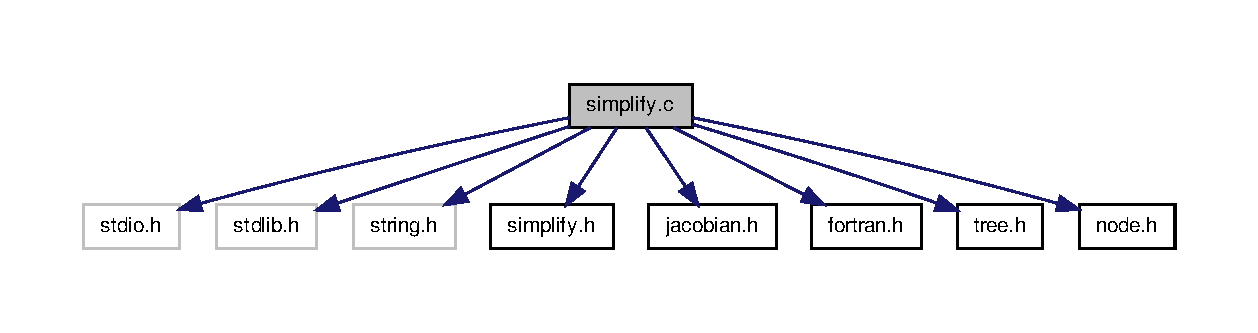
\includegraphics[width=350pt]{simplify_8c__incl}
\end{center}
\end{figure}
\subsection*{Macros}
\begin{DoxyCompactItemize}
\item 
\#define \hyperlink{simplify_8c_a369266c24eacffb87046522897a570d5}{\-\_\-\-G\-N\-U\-\_\-\-S\-O\-U\-R\-C\-E}
\end{DoxyCompactItemize}
\subsection*{Functions}
\begin{DoxyCompactItemize}
\item 
void \hyperlink{simplify_8c_a8eb4efb3974bdf6363238f4df2c8f7e3}{simplify\-Structure} (struct \hyperlink{structNode}{Node} $\ast$t)
\item 
void \hyperlink{simplify_8c_a03b5a4ee6f0130a2c38f54cea3016761}{S\-\_\-zero\-Assignments} (struct \hyperlink{structNode}{Node} $\ast$t)
\item 
void \hyperlink{simplify_8c_a6e2b9cdf29bedf48aba62a5034203f27}{register\-Zero\-Var} (char $\ast$s, int zero)
\item 
int \hyperlink{simplify_8c_a007c9cd2860c46f21184449737a510ad}{get\-Variable\-Zero} (char $\ast$s)
\item 
int \hyperlink{simplify_8c_a62e326df000e3ab3090552236e1aefe4}{S\-\_\-replace\-Zero\-Assignments} (struct \hyperlink{structNode}{Node} $\ast$t)
\item 
void \hyperlink{simplify_8c_a85016bba267f2b9d0914f4080c31ea7d}{S\-\_\-remove\-Plus\-Zero} (struct \hyperlink{structNode}{Node} $\ast$t)
\end{DoxyCompactItemize}


\subsection{Macro Definition Documentation}
\hypertarget{simplify_8c_a369266c24eacffb87046522897a570d5}{\index{simplify.\-c@{simplify.\-c}!\-\_\-\-G\-N\-U\-\_\-\-S\-O\-U\-R\-C\-E@{\-\_\-\-G\-N\-U\-\_\-\-S\-O\-U\-R\-C\-E}}
\index{\-\_\-\-G\-N\-U\-\_\-\-S\-O\-U\-R\-C\-E@{\-\_\-\-G\-N\-U\-\_\-\-S\-O\-U\-R\-C\-E}!simplify.c@{simplify.\-c}}
\subsubsection[{\-\_\-\-G\-N\-U\-\_\-\-S\-O\-U\-R\-C\-E}]{\setlength{\rightskip}{0pt plus 5cm}\#define \-\_\-\-G\-N\-U\-\_\-\-S\-O\-U\-R\-C\-E}}\label{simplify_8c_a369266c24eacffb87046522897a570d5}


\subsection{Function Documentation}
\hypertarget{simplify_8c_a007c9cd2860c46f21184449737a510ad}{\index{simplify.\-c@{simplify.\-c}!get\-Variable\-Zero@{get\-Variable\-Zero}}
\index{get\-Variable\-Zero@{get\-Variable\-Zero}!simplify.c@{simplify.\-c}}
\subsubsection[{get\-Variable\-Zero}]{\setlength{\rightskip}{0pt plus 5cm}int get\-Variable\-Zero (
\begin{DoxyParamCaption}
\item[{char $\ast$}]{s}
\end{DoxyParamCaption}
)}}\label{simplify_8c_a007c9cd2860c46f21184449737a510ad}
\hypertarget{simplify_8c_a6e2b9cdf29bedf48aba62a5034203f27}{\index{simplify.\-c@{simplify.\-c}!register\-Zero\-Var@{register\-Zero\-Var}}
\index{register\-Zero\-Var@{register\-Zero\-Var}!simplify.c@{simplify.\-c}}
\subsubsection[{register\-Zero\-Var}]{\setlength{\rightskip}{0pt plus 5cm}void register\-Zero\-Var (
\begin{DoxyParamCaption}
\item[{char $\ast$}]{s, }
\item[{int}]{zero}
\end{DoxyParamCaption}
)}}\label{simplify_8c_a6e2b9cdf29bedf48aba62a5034203f27}
\hypertarget{simplify_8c_a85016bba267f2b9d0914f4080c31ea7d}{\index{simplify.\-c@{simplify.\-c}!S\-\_\-remove\-Plus\-Zero@{S\-\_\-remove\-Plus\-Zero}}
\index{S\-\_\-remove\-Plus\-Zero@{S\-\_\-remove\-Plus\-Zero}!simplify.c@{simplify.\-c}}
\subsubsection[{S\-\_\-remove\-Plus\-Zero}]{\setlength{\rightskip}{0pt plus 5cm}void S\-\_\-remove\-Plus\-Zero (
\begin{DoxyParamCaption}
\item[{struct {\bf Node} $\ast$}]{t}
\end{DoxyParamCaption}
)}}\label{simplify_8c_a85016bba267f2b9d0914f4080c31ea7d}
\hypertarget{simplify_8c_a62e326df000e3ab3090552236e1aefe4}{\index{simplify.\-c@{simplify.\-c}!S\-\_\-replace\-Zero\-Assignments@{S\-\_\-replace\-Zero\-Assignments}}
\index{S\-\_\-replace\-Zero\-Assignments@{S\-\_\-replace\-Zero\-Assignments}!simplify.c@{simplify.\-c}}
\subsubsection[{S\-\_\-replace\-Zero\-Assignments}]{\setlength{\rightskip}{0pt plus 5cm}int S\-\_\-replace\-Zero\-Assignments (
\begin{DoxyParamCaption}
\item[{struct {\bf Node} $\ast$}]{t}
\end{DoxyParamCaption}
)}}\label{simplify_8c_a62e326df000e3ab3090552236e1aefe4}
\hypertarget{simplify_8c_a03b5a4ee6f0130a2c38f54cea3016761}{\index{simplify.\-c@{simplify.\-c}!S\-\_\-zero\-Assignments@{S\-\_\-zero\-Assignments}}
\index{S\-\_\-zero\-Assignments@{S\-\_\-zero\-Assignments}!simplify.c@{simplify.\-c}}
\subsubsection[{S\-\_\-zero\-Assignments}]{\setlength{\rightskip}{0pt plus 5cm}void S\-\_\-zero\-Assignments (
\begin{DoxyParamCaption}
\item[{struct {\bf Node} $\ast$}]{t}
\end{DoxyParamCaption}
)}}\label{simplify_8c_a03b5a4ee6f0130a2c38f54cea3016761}
\hypertarget{simplify_8c_a8eb4efb3974bdf6363238f4df2c8f7e3}{\index{simplify.\-c@{simplify.\-c}!simplify\-Structure@{simplify\-Structure}}
\index{simplify\-Structure@{simplify\-Structure}!simplify.c@{simplify.\-c}}
\subsubsection[{simplify\-Structure}]{\setlength{\rightskip}{0pt plus 5cm}void simplify\-Structure (
\begin{DoxyParamCaption}
\item[{struct {\bf Node} $\ast$}]{t}
\end{DoxyParamCaption}
)}}\label{simplify_8c_a8eb4efb3974bdf6363238f4df2c8f7e3}

\hypertarget{simplify_8h}{\section{simplify.\-h File Reference}
\label{simplify_8h}\index{simplify.\-h@{simplify.\-h}}
}
This graph shows which files directly or indirectly include this file\-:\nopagebreak
\begin{figure}[H]
\begin{center}
\leavevmode
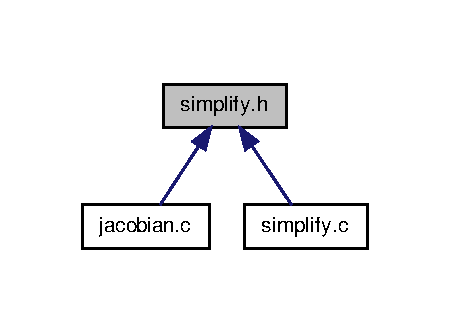
\includegraphics[width=216pt]{simplify_8h__dep__incl}
\end{center}
\end{figure}
\subsection*{Enumerations}
\begin{DoxyCompactItemize}
\item 
enum \hyperlink{simplify_8h_ae9d1253f6ec22141849cd8d6c51ce2b9}{Simplify\-State} \{ \hyperlink{simplify_8h_ae9d1253f6ec22141849cd8d6c51ce2b9a083e41952873b8835077428427331d46}{Zero\-Assignments} = 0, 
\hyperlink{simplify_8h_ae9d1253f6ec22141849cd8d6c51ce2b9a6cfc44c973b3f839e7f8566c20d29df5}{Replace\-Zero\-Assignments} = 1, 
\hyperlink{simplify_8h_ae9d1253f6ec22141849cd8d6c51ce2b9aa0bcf5ec205659d2bcd81b388435a124}{Remove\-Plus\-Zero} = 2
 \}
\end{DoxyCompactItemize}
\subsection*{Functions}
\begin{DoxyCompactItemize}
\item 
void \hyperlink{simplify_8h_a8eb4efb3974bdf6363238f4df2c8f7e3}{simplify\-Structure} (struct \hyperlink{structNode}{Node} $\ast$t)
\item 
void \hyperlink{simplify_8h_a605e2d45ead46a9f2d1da00d08032976}{register\-Zero\-Var} (char $\ast$name, int zero)
\item 
int \hyperlink{simplify_8h_a007c9cd2860c46f21184449737a510ad}{get\-Variable\-Zero} (char $\ast$s)
\item 
void \hyperlink{simplify_8h_a03b5a4ee6f0130a2c38f54cea3016761}{S\-\_\-zero\-Assignments} (struct \hyperlink{structNode}{Node} $\ast$t)
\item 
int \hyperlink{simplify_8h_a62e326df000e3ab3090552236e1aefe4}{S\-\_\-replace\-Zero\-Assignments} (struct \hyperlink{structNode}{Node} $\ast$t)
\item 
void \hyperlink{simplify_8h_a85016bba267f2b9d0914f4080c31ea7d}{S\-\_\-remove\-Plus\-Zero} (struct \hyperlink{structNode}{Node} $\ast$t)
\end{DoxyCompactItemize}
\subsection*{Variables}
\begin{DoxyCompactItemize}
\item 
enum \hyperlink{simplify_8h_ae9d1253f6ec22141849cd8d6c51ce2b9}{Simplify\-State} \hyperlink{simplify_8h_a5509be8af5ad302a2cd471067a767d91}{simplify\-State\-Size}
\end{DoxyCompactItemize}


\subsection{Enumeration Type Documentation}
\hypertarget{simplify_8h_ae9d1253f6ec22141849cd8d6c51ce2b9}{\index{simplify.\-h@{simplify.\-h}!Simplify\-State@{Simplify\-State}}
\index{Simplify\-State@{Simplify\-State}!simplify.h@{simplify.\-h}}
\subsubsection[{Simplify\-State}]{\setlength{\rightskip}{0pt plus 5cm}enum {\bf Simplify\-State}}}\label{simplify_8h_ae9d1253f6ec22141849cd8d6c51ce2b9}
\begin{Desc}
\item[Enumerator]\par
\begin{description}
\index{Zero\-Assignments@{Zero\-Assignments}!simplify.\-h@{simplify.\-h}}\index{simplify.\-h@{simplify.\-h}!Zero\-Assignments@{Zero\-Assignments}}\item[{\em 
\hypertarget{simplify_8h_ae9d1253f6ec22141849cd8d6c51ce2b9a083e41952873b8835077428427331d46}{Zero\-Assignments}\label{simplify_8h_ae9d1253f6ec22141849cd8d6c51ce2b9a083e41952873b8835077428427331d46}
}]\index{Replace\-Zero\-Assignments@{Replace\-Zero\-Assignments}!simplify.\-h@{simplify.\-h}}\index{simplify.\-h@{simplify.\-h}!Replace\-Zero\-Assignments@{Replace\-Zero\-Assignments}}\item[{\em 
\hypertarget{simplify_8h_ae9d1253f6ec22141849cd8d6c51ce2b9a6cfc44c973b3f839e7f8566c20d29df5}{Replace\-Zero\-Assignments}\label{simplify_8h_ae9d1253f6ec22141849cd8d6c51ce2b9a6cfc44c973b3f839e7f8566c20d29df5}
}]\index{Remove\-Plus\-Zero@{Remove\-Plus\-Zero}!simplify.\-h@{simplify.\-h}}\index{simplify.\-h@{simplify.\-h}!Remove\-Plus\-Zero@{Remove\-Plus\-Zero}}\item[{\em 
\hypertarget{simplify_8h_ae9d1253f6ec22141849cd8d6c51ce2b9aa0bcf5ec205659d2bcd81b388435a124}{Remove\-Plus\-Zero}\label{simplify_8h_ae9d1253f6ec22141849cd8d6c51ce2b9aa0bcf5ec205659d2bcd81b388435a124}
}]\end{description}
\end{Desc}


\subsection{Function Documentation}
\hypertarget{simplify_8h_a007c9cd2860c46f21184449737a510ad}{\index{simplify.\-h@{simplify.\-h}!get\-Variable\-Zero@{get\-Variable\-Zero}}
\index{get\-Variable\-Zero@{get\-Variable\-Zero}!simplify.h@{simplify.\-h}}
\subsubsection[{get\-Variable\-Zero}]{\setlength{\rightskip}{0pt plus 5cm}int get\-Variable\-Zero (
\begin{DoxyParamCaption}
\item[{char $\ast$}]{s}
\end{DoxyParamCaption}
)}}\label{simplify_8h_a007c9cd2860c46f21184449737a510ad}
\hypertarget{simplify_8h_a605e2d45ead46a9f2d1da00d08032976}{\index{simplify.\-h@{simplify.\-h}!register\-Zero\-Var@{register\-Zero\-Var}}
\index{register\-Zero\-Var@{register\-Zero\-Var}!simplify.h@{simplify.\-h}}
\subsubsection[{register\-Zero\-Var}]{\setlength{\rightskip}{0pt plus 5cm}void register\-Zero\-Var (
\begin{DoxyParamCaption}
\item[{char $\ast$}]{name, }
\item[{int}]{zero}
\end{DoxyParamCaption}
)}}\label{simplify_8h_a605e2d45ead46a9f2d1da00d08032976}
\hypertarget{simplify_8h_a85016bba267f2b9d0914f4080c31ea7d}{\index{simplify.\-h@{simplify.\-h}!S\-\_\-remove\-Plus\-Zero@{S\-\_\-remove\-Plus\-Zero}}
\index{S\-\_\-remove\-Plus\-Zero@{S\-\_\-remove\-Plus\-Zero}!simplify.h@{simplify.\-h}}
\subsubsection[{S\-\_\-remove\-Plus\-Zero}]{\setlength{\rightskip}{0pt plus 5cm}void S\-\_\-remove\-Plus\-Zero (
\begin{DoxyParamCaption}
\item[{struct {\bf Node} $\ast$}]{t}
\end{DoxyParamCaption}
)}}\label{simplify_8h_a85016bba267f2b9d0914f4080c31ea7d}
\hypertarget{simplify_8h_a62e326df000e3ab3090552236e1aefe4}{\index{simplify.\-h@{simplify.\-h}!S\-\_\-replace\-Zero\-Assignments@{S\-\_\-replace\-Zero\-Assignments}}
\index{S\-\_\-replace\-Zero\-Assignments@{S\-\_\-replace\-Zero\-Assignments}!simplify.h@{simplify.\-h}}
\subsubsection[{S\-\_\-replace\-Zero\-Assignments}]{\setlength{\rightskip}{0pt plus 5cm}int S\-\_\-replace\-Zero\-Assignments (
\begin{DoxyParamCaption}
\item[{struct {\bf Node} $\ast$}]{t}
\end{DoxyParamCaption}
)}}\label{simplify_8h_a62e326df000e3ab3090552236e1aefe4}
\hypertarget{simplify_8h_a03b5a4ee6f0130a2c38f54cea3016761}{\index{simplify.\-h@{simplify.\-h}!S\-\_\-zero\-Assignments@{S\-\_\-zero\-Assignments}}
\index{S\-\_\-zero\-Assignments@{S\-\_\-zero\-Assignments}!simplify.h@{simplify.\-h}}
\subsubsection[{S\-\_\-zero\-Assignments}]{\setlength{\rightskip}{0pt plus 5cm}void S\-\_\-zero\-Assignments (
\begin{DoxyParamCaption}
\item[{struct {\bf Node} $\ast$}]{t}
\end{DoxyParamCaption}
)}}\label{simplify_8h_a03b5a4ee6f0130a2c38f54cea3016761}
\hypertarget{simplify_8h_a8eb4efb3974bdf6363238f4df2c8f7e3}{\index{simplify.\-h@{simplify.\-h}!simplify\-Structure@{simplify\-Structure}}
\index{simplify\-Structure@{simplify\-Structure}!simplify.h@{simplify.\-h}}
\subsubsection[{simplify\-Structure}]{\setlength{\rightskip}{0pt plus 5cm}void simplify\-Structure (
\begin{DoxyParamCaption}
\item[{struct {\bf Node} $\ast$}]{t}
\end{DoxyParamCaption}
)}}\label{simplify_8h_a8eb4efb3974bdf6363238f4df2c8f7e3}


\subsection{Variable Documentation}
\hypertarget{simplify_8h_a5509be8af5ad302a2cd471067a767d91}{\index{simplify.\-h@{simplify.\-h}!simplify\-State\-Size@{simplify\-State\-Size}}
\index{simplify\-State\-Size@{simplify\-State\-Size}!simplify.h@{simplify.\-h}}
\subsubsection[{simplify\-State\-Size}]{\setlength{\rightskip}{0pt plus 5cm}enum {\bf Simplify\-State} simplify\-State\-Size}}\label{simplify_8h_a5509be8af5ad302a2cd471067a767d91}

\hypertarget{tree_8c}{\section{tree.\-c File Reference}
\label{tree_8c}\index{tree.\-c@{tree.\-c}}
}
{\ttfamily \#include $<$stdlib.\-h$>$}\\*
{\ttfamily \#include $<$stdio.\-h$>$}\\*
{\ttfamily \#include $<$string.\-h$>$}\\*
{\ttfamily \#include \char`\"{}tree.\-h\char`\"{}}\\*
{\ttfamily \#include \char`\"{}fortran.\-h\char`\"{}}\\*
{\ttfamily \#include \char`\"{}jacobian.\-h\char`\"{}}\\*
{\ttfamily \#include \char`\"{}node.\-h\char`\"{}}\\*
Include dependency graph for tree.\-c\-:\nopagebreak
\begin{figure}[H]
\begin{center}
\leavevmode
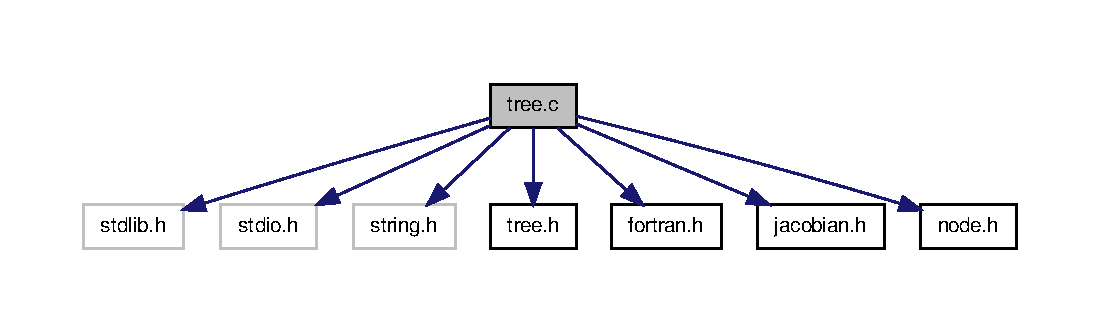
\includegraphics[width=350pt]{tree_8c__incl}
\end{center}
\end{figure}
\subsection*{Macros}
\begin{DoxyCompactItemize}
\item 
\#define \hyperlink{tree_8c_a369266c24eacffb87046522897a570d5}{\-\_\-\-G\-N\-U\-\_\-\-S\-O\-U\-R\-C\-E}
\end{DoxyCompactItemize}
\subsection*{Functions}
\begin{DoxyCompactItemize}
\item 
void $\ast$ \hyperlink{tree_8c_a2e8df70b0cd23ae836717e0219526e39}{emalloc} (size\-\_\-t nbytes)
\begin{DoxyCompactList}\small\item\em Nicer memory allocation function. \end{DoxyCompactList}\item 
void \hyperlink{tree_8c_a2c26e64b412545798ff08f0069cf2069}{fatal\-Error} (char $\ast$message)
\begin{DoxyCompactList}\small\item\em Fatal error function. \end{DoxyCompactList}\item 
void \hyperlink{tree_8c_ac1f744cdaf334ecc37399a3c066b8b36}{depth} (int d)
\item 
void \hyperlink{tree_8c_a4035da3929ae669ab801f4eff738bb6e}{print\-\_\-tree} (int d, struct \hyperlink{structNode}{Node} $\ast$t)
\begin{DoxyCompactList}\small\item\em Print a tree view of a \hyperlink{structNode}{Node}. \end{DoxyCompactList}\item 
struct \hyperlink{structVariable}{Variable} $\ast$ \hyperlink{tree_8c_a512919504f1e49ef80bd2309e300e0ab}{register\-Variable} (char $\ast$s, enum \hyperlink{tree_8h_ac62972ff1b21a037e56530cde67309ab}{Variable\-Type} tp)
\item 
char $\ast$ \hyperlink{tree_8c_a3020412eb1f21838ad4e159d6aa9d1c2}{process\-Identifier} (char $\ast$nm, enum \hyperlink{tree_8h_ac62972ff1b21a037e56530cde67309ab}{Variable\-Type} tp)
\item 
void \hyperlink{tree_8c_a8bf735ac7bae4295a443e9a0857559eb}{process\-Function\-Header} (struct \hyperlink{structNode}{Node} $\ast$f)
\item 
void \hyperlink{tree_8c_aa2d5d17ce59f6cf43cb57ce62d879e29}{process\-Dependent\-Vector\-Identifier} (char $\ast$s, struct \hyperlink{structNode}{Node} $\ast$rel)
\item 
struct \hyperlink{structNode}{Node} $\ast$ \hyperlink{tree_8c_a055e537e39403e6e3eab2415dd2428f9}{get\-Relative\-To\-Y} (char $\ast$s)
\end{DoxyCompactItemize}


\subsection{Macro Definition Documentation}
\hypertarget{tree_8c_a369266c24eacffb87046522897a570d5}{\index{tree.\-c@{tree.\-c}!\-\_\-\-G\-N\-U\-\_\-\-S\-O\-U\-R\-C\-E@{\-\_\-\-G\-N\-U\-\_\-\-S\-O\-U\-R\-C\-E}}
\index{\-\_\-\-G\-N\-U\-\_\-\-S\-O\-U\-R\-C\-E@{\-\_\-\-G\-N\-U\-\_\-\-S\-O\-U\-R\-C\-E}!tree.c@{tree.\-c}}
\subsubsection[{\-\_\-\-G\-N\-U\-\_\-\-S\-O\-U\-R\-C\-E}]{\setlength{\rightskip}{0pt plus 5cm}\#define \-\_\-\-G\-N\-U\-\_\-\-S\-O\-U\-R\-C\-E}}\label{tree_8c_a369266c24eacffb87046522897a570d5}


\subsection{Function Documentation}
\hypertarget{tree_8c_ac1f744cdaf334ecc37399a3c066b8b36}{\index{tree.\-c@{tree.\-c}!depth@{depth}}
\index{depth@{depth}!tree.c@{tree.\-c}}
\subsubsection[{depth}]{\setlength{\rightskip}{0pt plus 5cm}void depth (
\begin{DoxyParamCaption}
\item[{int}]{d}
\end{DoxyParamCaption}
)}}\label{tree_8c_ac1f744cdaf334ecc37399a3c066b8b36}
\hypertarget{tree_8c_a2e8df70b0cd23ae836717e0219526e39}{\index{tree.\-c@{tree.\-c}!emalloc@{emalloc}}
\index{emalloc@{emalloc}!tree.c@{tree.\-c}}
\subsubsection[{emalloc}]{\setlength{\rightskip}{0pt plus 5cm}void$\ast$ emalloc (
\begin{DoxyParamCaption}
\item[{size\-\_\-t}]{nbytes}
\end{DoxyParamCaption}
)}}\label{tree_8c_a2e8df70b0cd23ae836717e0219526e39}


Nicer memory allocation function. 

\hypertarget{tree_8c_a2c26e64b412545798ff08f0069cf2069}{\index{tree.\-c@{tree.\-c}!fatal\-Error@{fatal\-Error}}
\index{fatal\-Error@{fatal\-Error}!tree.c@{tree.\-c}}
\subsubsection[{fatal\-Error}]{\setlength{\rightskip}{0pt plus 5cm}void fatal\-Error (
\begin{DoxyParamCaption}
\item[{char $\ast$}]{message}
\end{DoxyParamCaption}
)}}\label{tree_8c_a2c26e64b412545798ff08f0069cf2069}


Fatal error function. 

Displays error {\itshape message} and then exits the application. 
\begin{DoxyParams}{Parameters}
{\em message} & Error message to display. \\
\hline
\end{DoxyParams}
\hypertarget{tree_8c_a055e537e39403e6e3eab2415dd2428f9}{\index{tree.\-c@{tree.\-c}!get\-Relative\-To\-Y@{get\-Relative\-To\-Y}}
\index{get\-Relative\-To\-Y@{get\-Relative\-To\-Y}!tree.c@{tree.\-c}}
\subsubsection[{get\-Relative\-To\-Y}]{\setlength{\rightskip}{0pt plus 5cm}struct {\bf Node}$\ast$ get\-Relative\-To\-Y (
\begin{DoxyParamCaption}
\item[{char $\ast$}]{s}
\end{DoxyParamCaption}
)}}\label{tree_8c_a055e537e39403e6e3eab2415dd2428f9}
\hypertarget{tree_8c_a4035da3929ae669ab801f4eff738bb6e}{\index{tree.\-c@{tree.\-c}!print\-\_\-tree@{print\-\_\-tree}}
\index{print\-\_\-tree@{print\-\_\-tree}!tree.c@{tree.\-c}}
\subsubsection[{print\-\_\-tree}]{\setlength{\rightskip}{0pt plus 5cm}void print\-\_\-tree (
\begin{DoxyParamCaption}
\item[{int}]{d, }
\item[{struct {\bf Node} $\ast$}]{t}
\end{DoxyParamCaption}
)}}\label{tree_8c_a4035da3929ae669ab801f4eff738bb6e}


Print a tree view of a \hyperlink{structNode}{Node}. 

\hypertarget{tree_8c_aa2d5d17ce59f6cf43cb57ce62d879e29}{\index{tree.\-c@{tree.\-c}!process\-Dependent\-Vector\-Identifier@{process\-Dependent\-Vector\-Identifier}}
\index{process\-Dependent\-Vector\-Identifier@{process\-Dependent\-Vector\-Identifier}!tree.c@{tree.\-c}}
\subsubsection[{process\-Dependent\-Vector\-Identifier}]{\setlength{\rightskip}{0pt plus 5cm}void process\-Dependent\-Vector\-Identifier (
\begin{DoxyParamCaption}
\item[{char $\ast$}]{s, }
\item[{struct {\bf Node} $\ast$}]{rel}
\end{DoxyParamCaption}
)}}\label{tree_8c_aa2d5d17ce59f6cf43cb57ce62d879e29}
\hypertarget{tree_8c_a8bf735ac7bae4295a443e9a0857559eb}{\index{tree.\-c@{tree.\-c}!process\-Function\-Header@{process\-Function\-Header}}
\index{process\-Function\-Header@{process\-Function\-Header}!tree.c@{tree.\-c}}
\subsubsection[{process\-Function\-Header}]{\setlength{\rightskip}{0pt plus 5cm}void process\-Function\-Header (
\begin{DoxyParamCaption}
\item[{struct {\bf Node} $\ast$}]{f}
\end{DoxyParamCaption}
)}}\label{tree_8c_a8bf735ac7bae4295a443e9a0857559eb}
\hypertarget{tree_8c_a3020412eb1f21838ad4e159d6aa9d1c2}{\index{tree.\-c@{tree.\-c}!process\-Identifier@{process\-Identifier}}
\index{process\-Identifier@{process\-Identifier}!tree.c@{tree.\-c}}
\subsubsection[{process\-Identifier}]{\setlength{\rightskip}{0pt plus 5cm}char$\ast$ process\-Identifier (
\begin{DoxyParamCaption}
\item[{char $\ast$}]{nm, }
\item[{enum {\bf Variable\-Type}}]{tp}
\end{DoxyParamCaption}
)}}\label{tree_8c_a3020412eb1f21838ad4e159d6aa9d1c2}
\hypertarget{tree_8c_a512919504f1e49ef80bd2309e300e0ab}{\index{tree.\-c@{tree.\-c}!register\-Variable@{register\-Variable}}
\index{register\-Variable@{register\-Variable}!tree.c@{tree.\-c}}
\subsubsection[{register\-Variable}]{\setlength{\rightskip}{0pt plus 5cm}struct {\bf Variable}$\ast$ register\-Variable (
\begin{DoxyParamCaption}
\item[{char $\ast$}]{s, }
\item[{enum {\bf Variable\-Type}}]{tp}
\end{DoxyParamCaption}
)}}\label{tree_8c_a512919504f1e49ef80bd2309e300e0ab}

\hypertarget{tree_8h}{\section{tree.\-h File Reference}
\label{tree_8h}\index{tree.\-h@{tree.\-h}}
}
This graph shows which files directly or indirectly include this file\-:\nopagebreak
\begin{figure}[H]
\begin{center}
\leavevmode
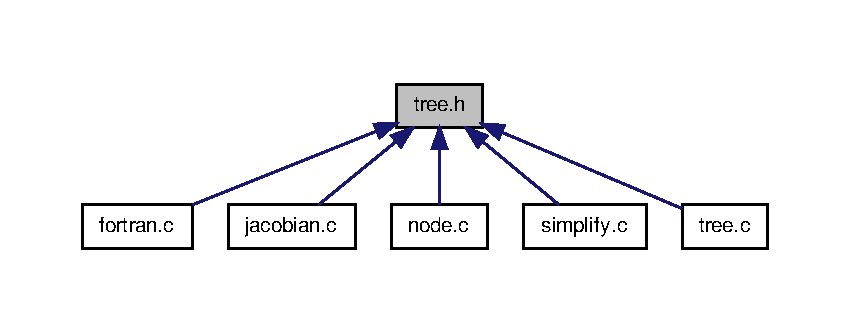
\includegraphics[width=350pt]{tree_8h__dep__incl}
\end{center}
\end{figure}
\subsection*{Data Structures}
\begin{DoxyCompactItemize}
\item 
struct \hyperlink{structVariable}{Variable}
\begin{DoxyCompactList}\small\item\em Datatype of a variable. \end{DoxyCompactList}\item 
struct \hyperlink{structFunction}{Function}
\begin{DoxyCompactList}\small\item\em Datatype of a function definition. \end{DoxyCompactList}\end{DoxyCompactItemize}
\subsection*{Macros}
\begin{DoxyCompactItemize}
\item 
\#define \hyperlink{tree_8h_a74e75242132eaabbc1c512488a135926}{M\-I\-N}(x, y)~(((x) $<$ (y)) ? (x) \-: (y))
\end{DoxyCompactItemize}
\subsection*{Enumerations}
\begin{DoxyCompactItemize}
\item 
enum \hyperlink{tree_8h_ac62972ff1b21a037e56530cde67309ab}{Variable\-Type} \{ \hyperlink{tree_8h_ac62972ff1b21a037e56530cde67309abaa8660a08a413e18977c553b09a26733d}{T\-D\-O\-U\-B\-L\-E}, 
\hyperlink{tree_8h_ac62972ff1b21a037e56530cde67309abac7f403f30660fcff1bc31cf1e20496c9}{T\-I\-N\-T}, 
\hyperlink{tree_8h_ac62972ff1b21a037e56530cde67309abaf3606f710a76d91a9d7f48b3604fb673}{T\-D\-O\-U\-B\-L\-E\-A\-R\-R\-A\-Y}
 \}
\begin{DoxyCompactList}\small\item\em \hyperlink{structVariable}{Variable} types. \end{DoxyCompactList}\end{DoxyCompactItemize}
\subsection*{Functions}
\begin{DoxyCompactItemize}
\item 
void $\ast$ \hyperlink{tree_8h_a2e8df70b0cd23ae836717e0219526e39}{emalloc} (size\-\_\-t nbytes)
\begin{DoxyCompactList}\small\item\em Nicer memory allocation function. \end{DoxyCompactList}\item 
void \hyperlink{tree_8h_a2c26e64b412545798ff08f0069cf2069}{fatal\-Error} (char $\ast$message)
\begin{DoxyCompactList}\small\item\em Fatal error function. \end{DoxyCompactList}\item 
void \hyperlink{tree_8h_a4035da3929ae669ab801f4eff738bb6e}{print\-\_\-tree} (int d, struct \hyperlink{structNode}{Node} $\ast$t)
\begin{DoxyCompactList}\small\item\em Print a tree view of a \hyperlink{structNode}{Node}. \end{DoxyCompactList}\item 
struct \hyperlink{structVariable}{Variable} $\ast$ \hyperlink{tree_8h_a512919504f1e49ef80bd2309e300e0ab}{register\-Variable} (char $\ast$s, enum \hyperlink{tree_8h_ac62972ff1b21a037e56530cde67309ab}{Variable\-Type} tp)
\item 
char $\ast$ \hyperlink{tree_8h_a3020412eb1f21838ad4e159d6aa9d1c2}{process\-Identifier} (char $\ast$nm, enum \hyperlink{tree_8h_ac62972ff1b21a037e56530cde67309ab}{Variable\-Type} tp)
\item 
void \hyperlink{tree_8h_aa2d5d17ce59f6cf43cb57ce62d879e29}{process\-Dependent\-Vector\-Identifier} (char $\ast$s, struct \hyperlink{structNode}{Node} $\ast$rel)
\item 
void \hyperlink{tree_8h_a8bf735ac7bae4295a443e9a0857559eb}{process\-Function\-Header} (struct \hyperlink{structNode}{Node} $\ast$f)
\item 
struct \hyperlink{structNode}{Node} $\ast$ \hyperlink{tree_8h_a055e537e39403e6e3eab2415dd2428f9}{get\-Relative\-To\-Y} (char $\ast$s)
\end{DoxyCompactItemize}
\subsection*{Variables}
\begin{DoxyCompactItemize}
\item 
F\-I\-L\-E $\ast$ \hyperlink{tree_8h_a7b668745fc4f8ed77aec0648aebf9058}{warn}
\item 
F\-I\-L\-E $\ast$ \hyperlink{tree_8h_a1277960b5f2b37137fe9b0b5a1ea0beb}{out}
\item 
int \hyperlink{tree_8h_a083bb88db3e0bb67c8410b9d89d11015}{labelcount}
\begin{DoxyCompactList}\small\item\em Counter for the label to use in the Fortran code. \end{DoxyCompactList}\item 
struct \hyperlink{structFunction}{Function} $\ast$ \hyperlink{tree_8h_a0fd22d424b64c2cec7bfee56806f173e}{func}
\begin{DoxyCompactList}\small\item\em Instance of the function definition. \end{DoxyCompactList}\item 
struct \hyperlink{structVariable}{Variable} $\ast$ \hyperlink{tree_8h_a2b48f6e35d13f38c37921e0991426c1c}{vars}
\begin{DoxyCompactList}\small\item\em Variables used in the O\-D\-E function. \end{DoxyCompactList}\end{DoxyCompactItemize}


\subsection{Macro Definition Documentation}
\hypertarget{tree_8h_a74e75242132eaabbc1c512488a135926}{\index{tree.\-h@{tree.\-h}!M\-I\-N@{M\-I\-N}}
\index{M\-I\-N@{M\-I\-N}!tree.h@{tree.\-h}}
\subsubsection[{M\-I\-N}]{\setlength{\rightskip}{0pt plus 5cm}\#define M\-I\-N(
\begin{DoxyParamCaption}
\item[{}]{x, }
\item[{}]{y}
\end{DoxyParamCaption}
)~(((x) $<$ (y)) ? (x) \-: (y))}}\label{tree_8h_a74e75242132eaabbc1c512488a135926}


\subsection{Enumeration Type Documentation}
\hypertarget{tree_8h_ac62972ff1b21a037e56530cde67309ab}{\index{tree.\-h@{tree.\-h}!Variable\-Type@{Variable\-Type}}
\index{Variable\-Type@{Variable\-Type}!tree.h@{tree.\-h}}
\subsubsection[{Variable\-Type}]{\setlength{\rightskip}{0pt plus 5cm}enum {\bf Variable\-Type}}}\label{tree_8h_ac62972ff1b21a037e56530cde67309ab}


\hyperlink{structVariable}{Variable} types. 

\begin{Desc}
\item[Enumerator]\par
\begin{description}
\index{T\-D\-O\-U\-B\-L\-E@{T\-D\-O\-U\-B\-L\-E}!tree.\-h@{tree.\-h}}\index{tree.\-h@{tree.\-h}!T\-D\-O\-U\-B\-L\-E@{T\-D\-O\-U\-B\-L\-E}}\item[{\em 
\hypertarget{tree_8h_ac62972ff1b21a037e56530cde67309abaa8660a08a413e18977c553b09a26733d}{T\-D\-O\-U\-B\-L\-E}\label{tree_8h_ac62972ff1b21a037e56530cde67309abaa8660a08a413e18977c553b09a26733d}
}]Double precision floating point variable. \index{T\-I\-N\-T@{T\-I\-N\-T}!tree.\-h@{tree.\-h}}\index{tree.\-h@{tree.\-h}!T\-I\-N\-T@{T\-I\-N\-T}}\item[{\em 
\hypertarget{tree_8h_ac62972ff1b21a037e56530cde67309abac7f403f30660fcff1bc31cf1e20496c9}{T\-I\-N\-T}\label{tree_8h_ac62972ff1b21a037e56530cde67309abac7f403f30660fcff1bc31cf1e20496c9}
}]Integer variable. \index{T\-D\-O\-U\-B\-L\-E\-A\-R\-R\-A\-Y@{T\-D\-O\-U\-B\-L\-E\-A\-R\-R\-A\-Y}!tree.\-h@{tree.\-h}}\index{tree.\-h@{tree.\-h}!T\-D\-O\-U\-B\-L\-E\-A\-R\-R\-A\-Y@{T\-D\-O\-U\-B\-L\-E\-A\-R\-R\-A\-Y}}\item[{\em 
\hypertarget{tree_8h_ac62972ff1b21a037e56530cde67309abaf3606f710a76d91a9d7f48b3604fb673}{T\-D\-O\-U\-B\-L\-E\-A\-R\-R\-A\-Y}\label{tree_8h_ac62972ff1b21a037e56530cde67309abaf3606f710a76d91a9d7f48b3604fb673}
}]Array of double precision variables. \end{description}
\end{Desc}


\subsection{Function Documentation}
\hypertarget{tree_8h_a2e8df70b0cd23ae836717e0219526e39}{\index{tree.\-h@{tree.\-h}!emalloc@{emalloc}}
\index{emalloc@{emalloc}!tree.h@{tree.\-h}}
\subsubsection[{emalloc}]{\setlength{\rightskip}{0pt plus 5cm}void$\ast$ emalloc (
\begin{DoxyParamCaption}
\item[{size\-\_\-t}]{nbytes}
\end{DoxyParamCaption}
)}}\label{tree_8h_a2e8df70b0cd23ae836717e0219526e39}


Nicer memory allocation function. 

\hypertarget{tree_8h_a2c26e64b412545798ff08f0069cf2069}{\index{tree.\-h@{tree.\-h}!fatal\-Error@{fatal\-Error}}
\index{fatal\-Error@{fatal\-Error}!tree.h@{tree.\-h}}
\subsubsection[{fatal\-Error}]{\setlength{\rightskip}{0pt plus 5cm}void fatal\-Error (
\begin{DoxyParamCaption}
\item[{char $\ast$}]{message}
\end{DoxyParamCaption}
)}}\label{tree_8h_a2c26e64b412545798ff08f0069cf2069}


Fatal error function. 

Displays error {\itshape message} and then exits the application. 
\begin{DoxyParams}{Parameters}
{\em message} & Error message to display. \\
\hline
\end{DoxyParams}
\hypertarget{tree_8h_a055e537e39403e6e3eab2415dd2428f9}{\index{tree.\-h@{tree.\-h}!get\-Relative\-To\-Y@{get\-Relative\-To\-Y}}
\index{get\-Relative\-To\-Y@{get\-Relative\-To\-Y}!tree.h@{tree.\-h}}
\subsubsection[{get\-Relative\-To\-Y}]{\setlength{\rightskip}{0pt plus 5cm}struct {\bf Node}$\ast$ get\-Relative\-To\-Y (
\begin{DoxyParamCaption}
\item[{char $\ast$}]{s}
\end{DoxyParamCaption}
)}}\label{tree_8h_a055e537e39403e6e3eab2415dd2428f9}
\hypertarget{tree_8h_a4035da3929ae669ab801f4eff738bb6e}{\index{tree.\-h@{tree.\-h}!print\-\_\-tree@{print\-\_\-tree}}
\index{print\-\_\-tree@{print\-\_\-tree}!tree.h@{tree.\-h}}
\subsubsection[{print\-\_\-tree}]{\setlength{\rightskip}{0pt plus 5cm}void print\-\_\-tree (
\begin{DoxyParamCaption}
\item[{int}]{d, }
\item[{struct {\bf Node} $\ast$}]{t}
\end{DoxyParamCaption}
)}}\label{tree_8h_a4035da3929ae669ab801f4eff738bb6e}


Print a tree view of a \hyperlink{structNode}{Node}. 

\hypertarget{tree_8h_aa2d5d17ce59f6cf43cb57ce62d879e29}{\index{tree.\-h@{tree.\-h}!process\-Dependent\-Vector\-Identifier@{process\-Dependent\-Vector\-Identifier}}
\index{process\-Dependent\-Vector\-Identifier@{process\-Dependent\-Vector\-Identifier}!tree.h@{tree.\-h}}
\subsubsection[{process\-Dependent\-Vector\-Identifier}]{\setlength{\rightskip}{0pt plus 5cm}void process\-Dependent\-Vector\-Identifier (
\begin{DoxyParamCaption}
\item[{char $\ast$}]{s, }
\item[{struct {\bf Node} $\ast$}]{rel}
\end{DoxyParamCaption}
)}}\label{tree_8h_aa2d5d17ce59f6cf43cb57ce62d879e29}
\hypertarget{tree_8h_a8bf735ac7bae4295a443e9a0857559eb}{\index{tree.\-h@{tree.\-h}!process\-Function\-Header@{process\-Function\-Header}}
\index{process\-Function\-Header@{process\-Function\-Header}!tree.h@{tree.\-h}}
\subsubsection[{process\-Function\-Header}]{\setlength{\rightskip}{0pt plus 5cm}void process\-Function\-Header (
\begin{DoxyParamCaption}
\item[{struct {\bf Node} $\ast$}]{f}
\end{DoxyParamCaption}
)}}\label{tree_8h_a8bf735ac7bae4295a443e9a0857559eb}
\hypertarget{tree_8h_a3020412eb1f21838ad4e159d6aa9d1c2}{\index{tree.\-h@{tree.\-h}!process\-Identifier@{process\-Identifier}}
\index{process\-Identifier@{process\-Identifier}!tree.h@{tree.\-h}}
\subsubsection[{process\-Identifier}]{\setlength{\rightskip}{0pt plus 5cm}char$\ast$ process\-Identifier (
\begin{DoxyParamCaption}
\item[{char $\ast$}]{nm, }
\item[{enum {\bf Variable\-Type}}]{tp}
\end{DoxyParamCaption}
)}}\label{tree_8h_a3020412eb1f21838ad4e159d6aa9d1c2}
\hypertarget{tree_8h_a512919504f1e49ef80bd2309e300e0ab}{\index{tree.\-h@{tree.\-h}!register\-Variable@{register\-Variable}}
\index{register\-Variable@{register\-Variable}!tree.h@{tree.\-h}}
\subsubsection[{register\-Variable}]{\setlength{\rightskip}{0pt plus 5cm}struct {\bf Variable}$\ast$ register\-Variable (
\begin{DoxyParamCaption}
\item[{char $\ast$}]{s, }
\item[{enum {\bf Variable\-Type}}]{tp}
\end{DoxyParamCaption}
)}}\label{tree_8h_a512919504f1e49ef80bd2309e300e0ab}


\subsection{Variable Documentation}
\hypertarget{tree_8h_a0fd22d424b64c2cec7bfee56806f173e}{\index{tree.\-h@{tree.\-h}!func@{func}}
\index{func@{func}!tree.h@{tree.\-h}}
\subsubsection[{func}]{\setlength{\rightskip}{0pt plus 5cm}struct {\bf Function}$\ast$ func}}\label{tree_8h_a0fd22d424b64c2cec7bfee56806f173e}


Instance of the function definition. 

\hypertarget{tree_8h_a083bb88db3e0bb67c8410b9d89d11015}{\index{tree.\-h@{tree.\-h}!labelcount@{labelcount}}
\index{labelcount@{labelcount}!tree.h@{tree.\-h}}
\subsubsection[{labelcount}]{\setlength{\rightskip}{0pt plus 5cm}int labelcount}}\label{tree_8h_a083bb88db3e0bb67c8410b9d89d11015}


Counter for the label to use in the Fortran code. 

\hypertarget{tree_8h_a1277960b5f2b37137fe9b0b5a1ea0beb}{\index{tree.\-h@{tree.\-h}!out@{out}}
\index{out@{out}!tree.h@{tree.\-h}}
\subsubsection[{out}]{\setlength{\rightskip}{0pt plus 5cm}F\-I\-L\-E$\ast$ out}}\label{tree_8h_a1277960b5f2b37137fe9b0b5a1ea0beb}
\hypertarget{tree_8h_a2b48f6e35d13f38c37921e0991426c1c}{\index{tree.\-h@{tree.\-h}!vars@{vars}}
\index{vars@{vars}!tree.h@{tree.\-h}}
\subsubsection[{vars}]{\setlength{\rightskip}{0pt plus 5cm}struct {\bf Variable}$\ast$ vars}}\label{tree_8h_a2b48f6e35d13f38c37921e0991426c1c}


Variables used in the O\-D\-E function. 

\hypertarget{tree_8h_a7b668745fc4f8ed77aec0648aebf9058}{\index{tree.\-h@{tree.\-h}!warn@{warn}}
\index{warn@{warn}!tree.h@{tree.\-h}}
\subsubsection[{warn}]{\setlength{\rightskip}{0pt plus 5cm}F\-I\-L\-E$\ast$ warn}}\label{tree_8h_a7b668745fc4f8ed77aec0648aebf9058}

%--- End generated contents ---

% Index
\newpage
\phantomsection
\addcontentsline{toc}{part}{Index}
\printindex

\end{document}
